\documentclass[11pt,a4paper,reqno]{amsart}

\usepackage[utf8]{inputenc}
\usepackage[T1]{fontenc}
\usepackage{lmodern}
\usepackage{amsmath,amssymb,amsthm}
\usepackage{mathtools}
\usepackage{graphicx}
\usepackage[margin=28mm]{geometry}
\usepackage{adjustbox}
\usepackage{array,booktabs}
\usepackage{enumitem}
\usepackage{xurl}
\usepackage[hidelinks]{hyperref}
\usepackage{orcidlink}
\usepackage{microtype}

\tolerance=2000
\emergencystretch=3em

\newtheorem{theorem}{Theorem}[section]
\newtheorem{lemma}[theorem]{Lemma}
\newtheorem{proposition}[theorem]{Proposition}
\newtheorem{corollary}[theorem]{Corollary}
\theoremstyle{definition}
\newtheorem{definition}[theorem]{Definition}
\newtheorem{conjecture}[theorem]{Conjecture}
\theoremstyle{remark}
\newtheorem{remark}[theorem]{Remark}

\newcommand{\R}{\mathbb{R}}
\newcommand{\Z}{\mathbb{Z}}
\newcommand{\C}{\mathbb{C}}
\newcommand{\Q}{\mathbb{Q}}
\newcommand{\PP}{\mathbb{P}}
\newcommand{\cL}{\mathcal{L}}
\newcommand{\cM}{\mathcal{M}}
\newcommand{\cS}{\mathcal{S}}
\newcommand{\cV}{\mathcal{V}}
\newcommand{\cO}{\mathcal{O}}
\newcommand{\Hom}{\operatorname{Hom}}
\newcommand{\End}{\operatorname{End}}
\newcommand{\Hess}{\operatorname{Hess}}
\newcommand{\Res}{\operatorname{Res}}
\newcommand{\rk}{\operatorname{rank}}
\newcommand{\ip}[2]{\langle #1,#2\rangle}
\newcommand{\bb}{\mathbf{b}}
\newcommand{\cc}{\mathbf{c}}
\newcommand{\va}{\mathbf{a}}
\newcommand{\ee}{\mathbf{e}}
\newcommand{\one}{\mathbf{1}}
\newcommand{\WP}{\mathrm{WP}}

% Archive identifiers of this revision.
\newcommand{\ownrelease}{v3.0.0}
\newcommand{\ownconceptdoi}{10.5281/zenodo.23567114}
\def\ownversiondoi{} % recorded after the Zenodo archive of the release is published

\title[Explicit string vacua and the Geometric Selection Conjecture]{Explicit String Vacua and the Geometric Selection Conjecture}

\author{Deep Bhattacharjee\,\orcidlink{0000-0003-0466-750X}}
\address{Formerly, Electro-Gravitational Space Propulsion Laboratory (EGSPL), Bhubaneswar, Odisha 751030, India}
\address{Formerly, University of Calcutta, Senate House, 87/1 College Street, Kolkata 700073, West Bengal, India}
\email{d.bhattacharjee@erl-forschung.de}
\email{itsdeep@live.com}
\email{egspl@proton.me}
\thanks{\sloppy Corresponding author: Deep Bhattacharjee. Email: \href{mailto:d.bhattacharjee@erl-forschung.de}{d.bhattacharjee@erl-forschung.de}, \href{mailto:itsdeep@live.com}{itsdeep@live.com}, \href{mailto:egspl@proton.me}{egspl@proton.me}; ORCID \href{https://orcid.org/0000-0003-0466-750X}{0000-0003-0466-750X}}
\author{Ushashi Bhattacharya\,\orcidlink{0009-0002-2254-3914}}
\address{Formerly, National Taiwan University, Taipei 106319, Taiwan}
\email{rai.bhattacharya.in@gmail.com}
\thanks{Ushashi Bhattacharya: email \href{mailto:rai.bhattacharya.in@gmail.com}{rai.bhattacharya.in@gmail.com}; ORCID \href{https://orcid.org/0009-0002-2254-3914}{0009-0002-2254-3914}.}

\subjclass[2020]{14J32; 81T30; 14J33; 32G20}
\keywords{heterotic compactification; Calabi--Yau threefold; Dwork pencil; line-bundle model}
\date{27 October 2026}

\begin{document}

\begin{abstract}
We combine explicit spectral calculations for the Dwork and weighted
Fermat pencils with an audit of the Geometric Selection Conjecture.
The residue calculation determines the character labels, cubic couplings
and invariant-direction mass maps, while an index argument excludes three
standard-embedding families on free quotients of thirteen hypergeometric
complete-intersection types. For a nonstandard construction we fix one
tetraquadric equation, prove smoothness and a free degree-four action,
and calculate equivariant bundle cohomology by an exact determinant
certificate. Its projected charged spectrum contains three families and
one Higgs doublet pair. At the specified split-bundle point, however, an
additional Abelian gauge factor survives, the perturbative Yukawa matrices
fail the required rank test, and the tree-level volume remains flat.
We then show that the first of these failures is forced: on every
Calabi--Yau threefold with at most four K\"ahler parameters, every
polystable sum of five line bundles with vanishing first Chern class has
a charge matrix of rank at most three and keeps at least one Abelian gauge
boson massless at its split locus. On the tetraquadric the polystable
K\"ahler classes of the fixed bundle form exactly the volume ray. For the
second failure we decide the perturbative selection rules on eleven split
data, the fixed bundle and ten further line-bundle sums with three families
on the same manifold, by a flow criterion for the singlet insertions: six
of the eleven lose a Yukawa matrix identically and five are not excluded.
We then follow the extension branch: a single non-split extension never
removes the forced gauge boson, while for the fixed bundle and five of the
ten further sums a polystable sum of two rank-two extensions and a line
bundle, with the same Chern character, exists on one side of a stability
wall arbitrarily close to the split point and carries no massless Abelian
gauge boson; for three further sums no such bundle exists at any K\"ahler
class, and for one it does not exist on the general tetraquadric. We fix
the acceptance windows for the stabilization, Yukawa and supersymmetry
breaking conditions, so that the conjecture becomes a definite statement,
and show that the failures found do not depend on them. No vacuum
satisfying all nine conditions is constructed; the Geometric Selection
Conjecture remains unproved.
\end{abstract}
\maketitle
\begingroup\small\noindent
\textit{Note.} An earlier and incomplete version of this work appeared in two
parts on Hexagon, as \href{https://hexagonmath.org/2610.00446v1}{2610.00446v1}
(the spectral calculations on the Dwork and weighted Fermat pencils) and
\href{https://hexagonmath.org/2610.00493v1}{2610.00493v1} (the mirror clause),
with the archived versions
\href{https://doi.org/10.5281/zenodo.23567115}{doi:10.5281/zenodo.23567115},
\href{https://doi.org/10.5281/zenodo.23646340}{doi:10.5281/zenodo.23646340}
and \href{https://doi.org/10.5281/zenodo.23647986}{doi:10.5281/zenodo.23647986}.
This version adds Section~\ref{sec:splitbranch}: the residual Abelian factor
is forced for every rank-five split bundle on a threefold with at most four
K\"ahler parameters, the polystable locus of the fixed bundle is the volume
ray, the perturbative selection rules are decided on eleven split data, and
the extension branch of the eleven data is decided for its two smallest
shapes; and Definition~\ref{def:windows}, which fixes the acceptance
windows of the three phenomenological conditions.
The programs that check the finite arithmetic are in the repository
\href{https://github.com/creelie/geometric-selection-conjecture}{\texttt{creelie/geometric-selection-conjecture}} on GitHub, release
\ownrelease{}, concept DOI
\href{https://doi.org/\ownconceptdoi}{\ownconceptdoi}\ifx\ownversiondoi\empty\else,
version DOI \href{https://doi.org/\ownversiondoi}{\ownversiondoi}\fi.
\par\endgroup\medskip

\section{Introduction}\label{sec:intro}
The physical problem has two distinct levels. One can calculate a
spectrum and cubic form on a specified Calabi--Yau family. One can also
ask for a single compactification satisfying the gauge, matter, mass,
stabilization and supersymmetry requirements C1--C9. The first calculation
is not a solution to the second existence problem.

This paper brings together the spectral calculations on the Dwork and
weighted Fermat pencils, the mirror restriction of the selector, and the
construction criteria for the conjecture, in one narrative with one
bibliography. The three strands are kept apart where they must be: the
Dwork mass matrix below is not substituted for a Yukawa matrix of the
tetraquadric bundle later in the paper.

The fixed-candidate calculation is
Theorems~\ref{thm:fixedquotient} and~\ref{thm:fixedcohom}:
a single equation at the parameter $\theta=\pi$ gives a smooth free
quotient, with a rank-five bundle of index $-3$ and explicitly projected
charged spectrum. The use of a transcendental coefficient certifies
avoidance of algebraic bad parameters; it does not stabilize that
coefficient. The line-bundle model originates in \cite{BCL}.
The determinant and explicit seed identities make the chosen
complex structure auditable without assuming it is generic.
Section~\ref{sec:splitbranch} then shows that the two failures found at
that point are not accidents of the choice: the residual Abelian factor
is forced for every sum of five line bundles on a threefold with at most
four K\"ahler parameters (Theorem~\ref{thm:forced}), and the perturbative
selection rules, decided by a flow criterion, exclude six of eleven split
data on the tetraquadric and leave five (Proposition~\ref{prop:eleven}).
The same section follows the extension branch away from the split locus:
one non-split extension never removes the forced gauge boson
(Proposition~\ref{prop:oneblock}), while a polystable sum of two rank-two
extensions and a line bundle does so for the fixed datum and five of the
ten further data, on one side of a stability wall through the polystable
point, and is excluded for the other four at every K\"ahler class or on
the general tetraquadric (Theorem~\ref{thm:twoblocks}).
Definition~\ref{def:windows} fixes the acceptance windows of C7--C9, so
that the conjecture is the definite statement GSC$(W)$ of
Conjecture~\ref{conj:gscw}; the negative results do not depend on the
windows. Section~\ref{sec:ledger} tests the fixed datum against every
condition. It records both verified statements and failures.

For comparison, consider the Dwork family
\begin{equation}\label{eq:dwork}
 X_\psi=\{\textstyle\sum_{i=1}^5 x_i^5-5\psi\prod_{i=1}^5x_i=0\}
 \subset\PP^4,\qquad\psi^5\ne1.
\end{equation}
The standard-embedding $E_6$ theory has $101$ charged $\mathbf{27}$'s,
not three Standard Model families. In the next statements ``generation''
denotes one such $E_6$ multiplet. The group of diagonal phases is
$\Gamma\cong(\Z/5)^3$; the notation is local to these pencil sections
and will later be reused for the separate tetraquadric group.


\begin{theorem}[Labels]\label{thm:A}
The hundred and one classes carry hundred and one distinct characters of
$\Gamma$, each with multiplicity one, so every generation is labelled by
its character. Of the hundred and twenty-five characters of $\Gamma$ the
twenty-four that do not occur are exactly the classes of the permutations
of $(0,1,2,3,4)$. The permutation group $S_5$ of the coordinates permutes
the labels in five orbits of sizes $1$, $20$, $20$, $30$ and $30$, the five
types of generation.
\end{theorem}

\begin{theorem}[Couplings]\label{thm:B}
Let $\psi^5\ne1$. The cubic form of the pencil, normalised so that the
monomial $x_1^3\cdots x_5^3$ has value one, takes on three generations
$\va,\bb,\cc$ the value $\psi^{r}$ when $\va+\bb+\cc\equiv(3-r)\one\pmod 5$
for some $r\in\{0,1,2,3\}$, and zero otherwise. There are $1431$ unordered
triples with a nonzero coupling, $566$, $425$, $280$ and $160$ of them with
$r=0,1,2,3$, and all $1431$ are nonzero at every smooth member with
$\psi\ne0$.
\end{theorem}

\begin{theorem}[Mass map]\label{thm:C}
The invariant class $h=x_1x_2x_3x_4x_5$, the direction of the pencil
itself, pairs each generation $\bb$ with exactly one generation
$\sigma(\bb)$, where $\sigma$ is an involution of the labels with one fixed
point. The coupling of $h$, $\bb$ and $\sigma(\bb)$ equals $1$ for the
fifty-one labels with all entries at most two, $\psi$ for the thirty labels
of type $(3,1,1,0,0)$ and $\psi^2$ for the twenty labels of type
$(3,2,0,0,0)$. Hence the holomorphic mass map induced by a vacuum value of the
$\mathbf{27}$ labelled by $h$ has full rank one hundred and one for every
$\psi\ne0$, $\psi^5\ne1$, its determinant is $\psi^{70}$, and at the
Fermat point $\psi=0$ its rank is fifty-one with the fifty generations
containing an exponent three massless. The spectrum consists of one singlet
and fifty doublets, and the $\Gamma$-invariant metric is diagonal in the
labels, so the fifty doublet masses are, in units of the vacuum value,
$|\psi|^{r(\bb)}\big(g_{\bb}\,g_{\sigma(\bb)}\big)^{-1/2}$ with $g$ the
Hodge norms of the classes.
\end{theorem}



The same residue and character questions extend to three weighted families
of Fermat type, the pencils
\begin{equation}\label{eq:wpencil}
X_\psi=\Big\{\sum_{i=1}^5x_i^{n_i}-d\psi\,x_1x_2x_3x_4x_5=0\Big\}
\subset\PP(w),\qquad n_i=\frac{d}{w_i},
\end{equation}
of sextics in $\PP(1,1,1,1,2)$, octics in $\PP(1,1,1,1,4)$ and dectics in
$\PP(1,1,1,2,5)$, whose periods and mirror maps were computed by
Morrison~\cite{Mor92}, Klemm and Theisen~\cite{KT93} and
Font~\cite{Fon93}. Here $d=\sum_iw_i$ is $6$, $8$ and $10$, each member
with $\psi^d\delta\ne1$, where $\delta=\prod_iw_i^{w_i}$ is $4$, $256$ and
$12\,500$, is smooth, and the group $\Gamma$ of diagonal phases preserving
the pencil has order $108$, $128$ and $100$. The answer is different there.

\begin{theorem}[Weighted pencils]\label{thm:E}
Let $X_\psi$ be the sextic, octic or dectic pencil \eqref{eq:wpencil} with
$\psi^d\delta\ne1$. Then $X_\psi$ is a smooth Calabi--Yau threefold with
$h^{1,1}=1$ and $h^{2,1}=103$, $149$ and $145$, and the following hold.
\begin{enumerate}[label=\textup{(\roman*)},leftmargin=*,itemsep=1pt]
\item The generations are the monomials $x^{\bb}$ of weighted degree $d$
with $0\le b_i\le n_i-2$, but they carry only $96$, $122$ and $100$
distinct characters of $\Gamma$: $7$, $27$ and $42$ classes of two or three
generations share a character.
\item The cubic form, normalised so that $\prod_ix_i^{n_i-2}$ has value
one, takes on three generations $\va,\bb,\cc$ the value
$\psi^r\prod_iw_i^{k_i}$ when $a_i+b_i+c_i=n_i-2-r+n_ik_i$ for every $i$,
with $r\in\{0,\dots,d-1\}$ and integers $k_i\ge0$, and zero otherwise; for
$\psi\ne0$ every coupling allowed by $\Gamma$ is nonzero.
\item For $\psi\ne0$ the mass map of the invariant direction has rank
$99$, $125$ and $109$, so that $4$, $24$ and $36$ generations stay massless
at every member; at $\psi=0$ its rank is $44$, $85$ and $72$.
\item No member, and no quotient of a member by a group acting freely,
carries three families with the standard embedding.
\end{enumerate}
\end{theorem}




These results are proved in Sections~\ref{sec:dictionary}--\ref{sec:weighted}
and their appendices. They concern specified holomorphic maps and
their stated metric normalization, not a completed phenomenological
vacuum. The global family-index obstruction is strengthened in
Section~\ref{sec:freequot}. The GSC construction problem is formulated
in Section~\ref{sec:selection}, and the one-candidate audit follows.


\section{The dictionary}\label{sec:dictionary}

Throughout, $X$ is a compact K\"ahler threefold with holonomy exactly
$SU(3)$, so that $X$ has a Ricci-flat K\"ahler metric $g$ by Yau's
theorem, a nowhere vanishing holomorphic three-form $\Omega$, and
$h^{1,0}=h^{2,0}=0$. The tangent bundle $T_X$ with the Levi-Civita
connection is a holomorphic $SU(3)$-bundle with a Hermitian Yang--Mills
connection; this is the standard embedding.

\subsection{Spinors and the Dolbeault complex}

On a K\"ahler manifold of complex dimension $n$ with trivial canonical
bundle the spinor bundle is $S=\bigoplus_{q}\Lambda^{0,q}T^*_X$, and the
Dirac operator of the Levi-Civita connection is $D=\sqrt2(\bar\partial+
\bar\partial^*)$, with the chirality grading given by the parity of $q$
(Hitchin~\cite{Hit74}). If $V$ is a holomorphic Hermitian bundle with a
connection whose curvature is of type $(1,1)$, the Dirac operator twisted by
$V$ is $\sqrt2(\bar\partial_V+\bar\partial_V^*)$ on $\Lambda^{0,\bullet}
\otimes V$, and its kernel is the harmonic representative of
$\bigoplus_q H^{0,q}(X,V)$. This is the only input from spin geometry.

\subsection{The charged spectrum}

\begin{theorem}[Spectrum of the standard embedding]\label{thm:dictionary}
Let $X$ be as above with the standard embedding. The massless charged
chiral multiplets of the $E_8\times E_8$ heterotic string on $\R^{3,1}
\times X$ in the observable sector transform under $E_6$ as
\[
h^{2,1}(X)\ \text{copies of }\mathbf{27}\ \oplus\ h^{1,1}(X)\ \text{copies of
}\overline{\mathbf{27}},
\]
with the $\mathbf{27}$'s in natural bijection with $H^1(X,T_X)\cong
H^{2,1}(X)$ and the $\overline{\mathbf{27}}$'s with $H^1(X,T_X^*)\cong
H^{1,1}(X)$. The net number of generations is
$|h^{2,1}-h^{1,1}|=\tfrac12|\chi(X)|$.
\end{theorem}

\begin{proof}
The ten-dimensional gaugino is a Majorana--Weyl spinor with values in the
adjoint of $E_8$. Under $E_8\supset E_6\times SU(3)$,
\[
\mathbf{248}=(\mathbf{78},\mathbf1)\oplus(\mathbf1,\mathbf8)\oplus
(\mathbf{27},\mathbf3)\oplus(\overline{\mathbf{27}},\bar{\mathbf3}),
\]
and the standard embedding identifies the $SU(3)$ factor with the holonomy
group acting on $T_X$ and sends $\mathbf3$ to $T_X$, $\bar{\mathbf3}$ to
$T_X^*$. A ten-dimensional Weyl spinor on $\R^{3,1}\times X$ decomposes as
a four-dimensional Weyl spinor times a six-dimensional one of correlated
chirality, so the four-dimensional massless chiral fermions in the
$\mathbf{27}$ are the zero modes of the Dirac operator on $X$ twisted by
$T_X$, counted with their six-dimensional chirality; the $SU(3)$ holonomy
makes the twisted operator $\sqrt2(\bar\partial+\bar\partial^*)$ on
$\Lambda^{0,\bullet}\otimes T_X$, and its chiral zero modes are
$H^{0,1}(X,T_X)\oplus H^{0,3}(X,T_X)$ and $H^{0,0}(X,T_X)\oplus
H^{0,2}(X,T_X)$ for the two chiralities. Since $\Omega$ trivialises
$\Lambda^3T_X^*$, contraction with $\Omega$ gives $H^{0,q}(X,T_X)\cong
H^{2,q}(X)$ and $H^{0,q}(X,T_X^*)=H^{1,q}(X)$. With $h^{2,0}=h^{1,0}=0$
and Serre duality, $H^{0,0}(T_X)=H^{2,0}=0$, $H^{0,3}(T_X)=
H^{2,3}=\overline{H^{1,0}}^*=0$, $H^{0,2}(T_X)=H^{2,2}\cong
\overline{H^{1,1}}$, and $H^{0,1}(T_X)=H^{2,1}$. A four-dimensional Weyl
fermion in the $\mathbf{27}$ of one chirality and one in the
$\overline{\mathbf{27}}$ of the opposite chirality are related by
conjugation, so the chiral multiplets of definite four-dimensional
chirality are $h^{2,1}$ copies of $\mathbf{27}$ from $H^{0,1}(T_X)$ and
$h^{1,1}$ copies of $\overline{\mathbf{27}}$ from $H^{0,2}(T_X)$. The index
of the twisted Dirac operator is $h^{2,1}-h^{1,1}$, which equals $-\chi(X)/2$
because $\chi=2(h^{1,1}-h^{2,1})$ on a threefold with $h^{1,0}=h^{2,0}=0$.
\end{proof}

\subsection{The cubic form}

Let $V=H^1(X,T_X)$. The composition of cup product and contraction,
\[
V\otimes V\otimes V\to H^3(X,\Lambda^3T_X)=H^3(X,K_X^{-1})\cong
H^3(X,\cO_X)\cong\C,
\]
where the last two isomorphisms use $\Omega$, is a symmetric trilinear form
$Y$ on $V$, the cubic form of $X$. In terms of the variation of Hodge
structure, with $\nabla$ the Gauss--Manin connection and $\Omega$ extended
holomorphically over the moduli space,
\begin{equation}\label{eq:yukawa}
Y(a,b,c)=\int_X\Omega\wedge\nabla_a\nabla_b\nabla_c\Omega,
\end{equation}
and this is the coupling of three $\mathbf{27}$'s~\cite{Str85}. Changing
$\Omega$ to $f\Omega$ multiplies $Y$ by $f^2$, so only the cubic form up to
a nowhere vanishing holomorphic function is intrinsic, and the physical
couplings are $Y$ divided by the square roots of the Hodge norms of the three
classes and by $\ip{\Omega}{\overline\Omega}$~\cite{DKL90,CdlO91}.

\subsection{Mass terms}

A vacuum value $v$ of the scalar in the $\mathbf{27}$ labelled by a class
$h\in V$ in a direction that breaks $E_6$ gives, through the superpotential
$Y(h,\cdot,\cdot)$, a Dirac mass term $v\,Y(h,b,c)$ between the fermions
labelled by $b$ and $c$~\cite{Wit85}. The physical mass matrix is
\begin{equation}\label{eq:massmatrix}
M_{bc}=v\,\frac{Y(h,b,c)}{\sqrt{g_{b}\,g_{c}}}
\end{equation}
in an orthogonal basis of $V$, where $g_b=\ip{\omega_b}{\overline{\omega_b}}$
is the Hodge norm of the harmonic representative, and the masses are its
singular values. We call $Y(h,\cdot,\cdot)$ the mass map of $h$.

\subsection{Hypersurfaces}

For a smooth hypersurface $X=\{F=0\}\subset\PP^4$ of degree five let
$J_F=(\partial_1F,\dots,\partial_5F)$ be the Jacobian ideal and
$R=\C[x_1,\dots,x_5]/J_F$ the Jacobian ring, graded by degree. Griffiths'
theorem~\cite{Gri69} identifies $H^{3-q,q}_{\mathrm{prim}}(X)$ with
$R_{5(q+1)-5}$ through residues: for a homogeneous $P$ of degree $5q$,
\[
\omega_P=\Res_X\frac{P\,\Omega_0}{F^{q+1}},\qquad
\Omega_0=\sum_i(-1)^{i}x_i\,dx_1\wedge\cdots\widehat{dx_i}\cdots\wedge dx_5,
\]
so $H^{3,0}=R_0$, $H^{2,1}=R_5$, $H^{1,2}=R_{10}$, $H^{0,3}=R_{15}$, and
every class of a quintic threefold is primitive in degree three. The ring
$R$ is a graded complete intersection with Hilbert series
$(1+t+t^2+t^3)^5$, so $\dim R_5=101$, $\dim R_{15}=1$, and $R_{15}$ is the
socle. Macaulay's theorem, as stated in~\cite{CG80}, says that the Hessian
$\Hess F=\det(\partial_i\partial_jF)$ has nonzero image in $R_{15}$ and
that the cubic form is multiplication in $R$ followed by the residue
functional $\lambda_F:R_{15}\to\C$, $\lambda_F(\Hess F)=1$, up to a
constant depending only on the normalisation of $\Omega$:
\begin{equation}\label{eq:jacobianyukawa}
Y(\omega_P,\omega_Q,\omega_S)=c\,\lambda_F(PQS).
\end{equation}
Figure~\ref{fig:hodge} shows a curve on the Fermat quintic and the Hodge
numbers of a quintic threefold: by Theorem~\ref{thm:dictionary} the hundred and one classes
of type $(2,1)$ are the generations and the single class of type $(1,1)$
is the antigeneration.

\begin{figure}[t]
\centering
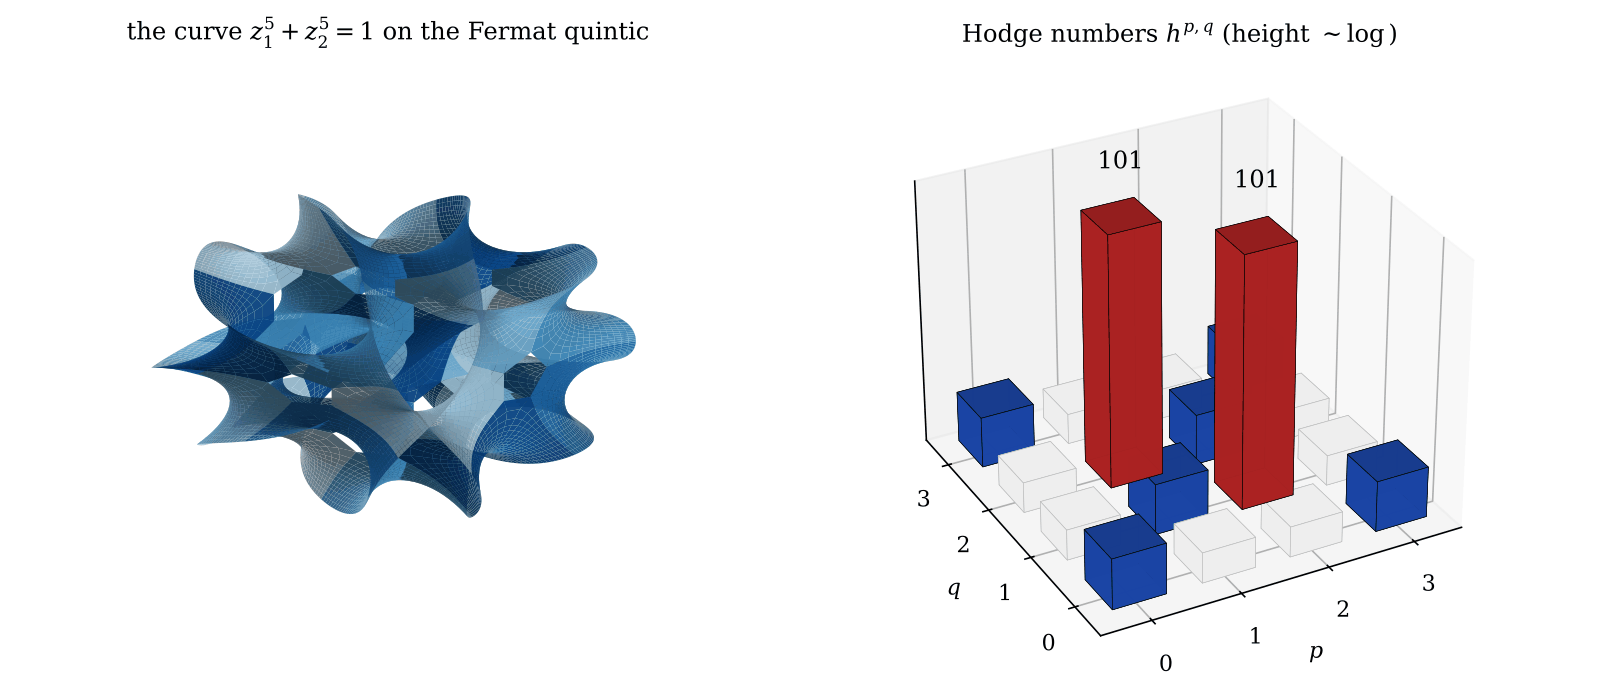
\includegraphics[width=0.96\textwidth]{figures/fig_hodge.png}
\caption{Left: the intersection of the Fermat quintic with the plane
$x_3=x_4=0$, which in an affine chart is the curve $z_1^5+z_2^5=1$ in
$\C^2$, drawn with the parametrisation of Hanson~\cite{Han94} and projected
to three dimensions along $(\mathrm{Re}\,z_1,\mathrm{Re}\,z_2,
\cos\alpha\,\mathrm{Im}\,z_1+\sin\alpha\,\mathrm{Im}\,z_2)$. It is
assembled from twenty-five patches, one for each pair of fifth roots of
unity; $\Gamma$ preserves the curve and acts on it through
$\mu_5\times\mu_5$, permuting the patches. Right:
the Hodge numbers $h^{p,q}$ of a smooth quintic threefold, with height
proportional to $1+\log_2h^{p,q}$; the six blue bars have height one, the
two red bars are $h^{2,1}=h^{1,2}=101$, and the grey cells are zero.}
\label{fig:hodge}
\end{figure}

\section{Labels}\label{sec:labels}

Let $\zeta=e^{2\pi i/5}$ and let $K=\{a\in(\Z/5)^5:\sum a_i=0\}$ act on
$\PP^4$ by $x_i\mapsto\zeta^{a_i}x_i$. The diagonal subgroup $D$ acts
trivially on $\PP^4$, and $\Gamma=K/D\cong(\Z/5)^3$ preserves $F_\psi=
\sum x_i^5-5\psi\prod x_i$ for every $\psi$. The characters of $\Gamma$ are
the characters of $K$ trivial on $D$, that is the classes
\[
\widehat\Gamma=\{\bb\in(\Z/5)^5:\textstyle\sum b_i=0\}/\langle\one\rangle,
\qquad |\widehat\Gamma|=125,
\]
with $\bb$ acting by $a\mapsto\zeta^{a\cdot\bb}$. A monomial $x^{\bb}$
transforms under $a\in K$ by $\zeta^{a\cdot\bb}$, so it lies in the isotypic
component of the class of $\bb$.

Let $B$ be the set of $\bb\in\{0,1,2,3\}^5$ with $|\bb|=\sum b_i=5$. The
monomials $x^{\bb}$, $\bb\in B$, are a basis of $R_5$ for $\psi^5\ne1$,
because the Jacobian ideal of $F_\psi$ is generated by $x_i^4-\psi\prod_{j
\ne i}x_j$, and modulo these every monomial reduces to one with all
exponents at most three; the reduced monomials of degree five are the
$101$ elements of $B$, which matches $\dim R_5$. The count is the number of
compositions of five into five parts, $\binom94=126$, less the twenty with
a part equal to four and the five with a part equal to five.

\begin{proof}[Proof of Theorem~\ref{thm:A}]
Two elements $\bb,\bb'\in B$ define the same character when
$\bb'\equiv\bb+k\one\pmod5$ for some $k$. Since the entries of $\bb'$ lie in
$\{0,\dots,4\}$, $\bb'$ is the vector of residues of $\bb+k\one$ in that
range: each $b'_i$ is $b_i+k$ or $b_i+k-5$, and $\sum b'_i=5$. For $k=1$ the
residues are $b_i+1\le4$ unless $b_i=4$, impossible, so all residues are
$b_i+1$, with sum $10\ne5$. For $k=2$ the residues are $b_i+2$ if $b_i\le2$
and $b_i-3$ if $b_i=3$; the sum is $15-5m$ where $m$ is the number of
threes, so $m=2$, but two threes already sum to six. For $k=3$ the residues
are $b_i+3$ if $b_i\le1$ and $b_i-2$ if $b_i\ge2$, sum $20-5m'$ with $m'$
the number of entries at least two, so $m'=3$, three entries at least two
summing to at most five, impossible. For $k=4$ the residues are $b_i+4$ if
$b_i=0$ and $b_i-1$ otherwise, sum $25-5m''$ with $m''$ the number of
nonzero entries, so $m''=4$: four nonzero entries summing to five means
$(2,1,1,1,0)$ up to order, and then $\bb'=(1,0,0,0,4)$ has a four. So only
$k=0$ works and the $101$ characters are distinct; being characters of an
abelian group acting on $R_5$, they are then the full decomposition, each
isotypic component being one-dimensional.

The group $\widehat\Gamma$ has $125$ elements and $B$ realises $101$ of
them, so exactly $24$ are missed. A permutation of $(0,1,2,3,4)$ has sum
ten, so its class lies in $\widehat\Gamma$, and adding $\one$ to it gives
another permutation of $(0,1,2,3,4)$ modulo five; the hundred and twenty
permutations therefore fall into $24$ classes of five. None of these classes
meets $B$, because every representative with entries in $\{0,\dots,4\}$
is a permutation of $(0,1,2,3,4)$ and contains a four. Hence the $24$ missed
classes are exactly the classes of the permutations.

Finally $S_5$ permutes the exponent vectors, and the orbits in $B$ are the
multisets of entries: $\{1,1,1,1,1\}$ (one element), $\{2,1,1,1,0\}$
(twenty), $\{3,2,0,0,0\}$ (twenty), $\{2,2,1,0,0\}$ (thirty) and
$\{3,1,1,0,0\}$ (thirty).
\end{proof}

Figure~\ref{fig:labels} shows the hundred and one labels.

\begin{figure}[t]
\centering
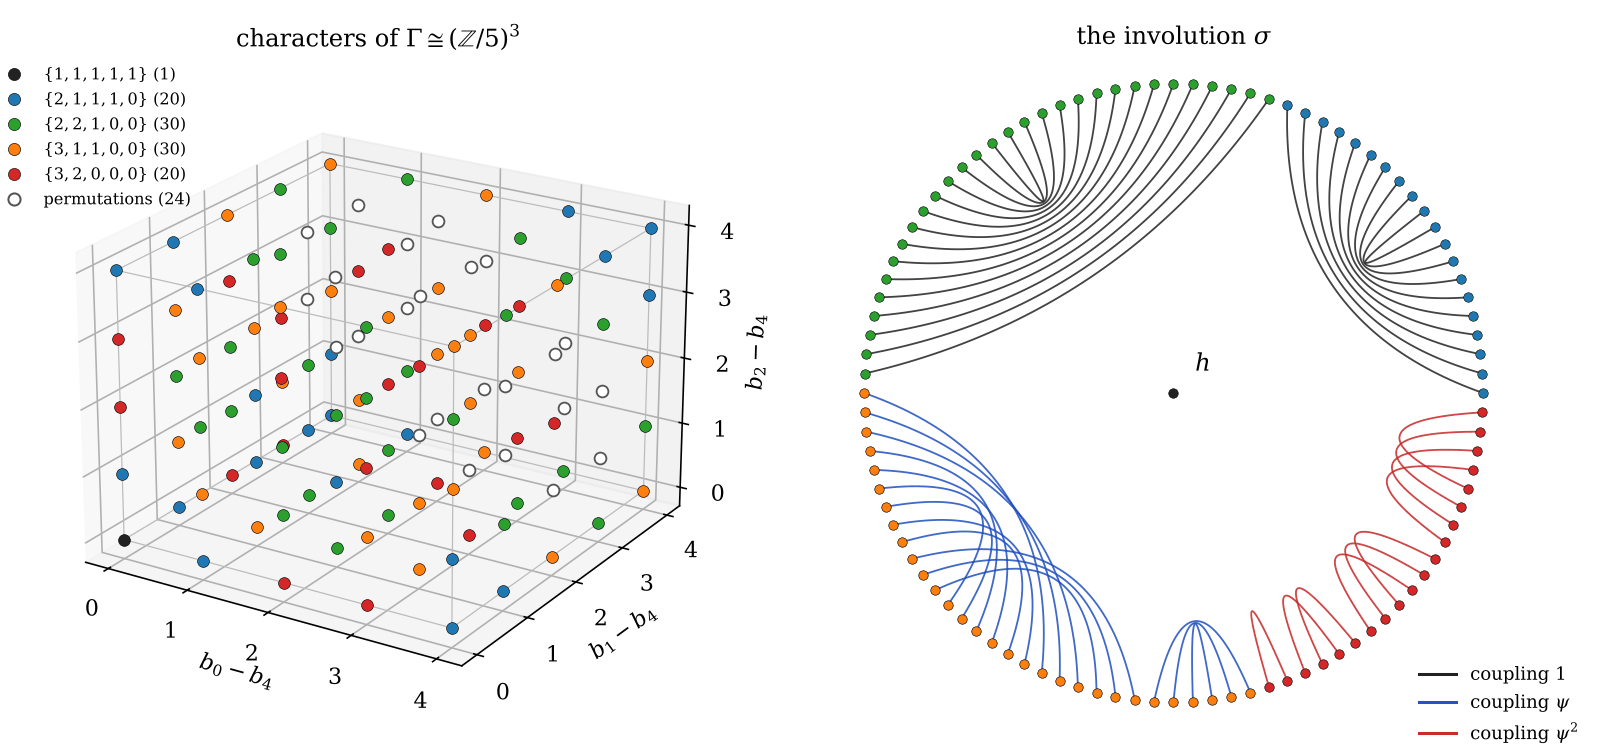
\includegraphics[width=0.96\textwidth]{figures/fig_labels.png}
\caption{The hundred and one generations of the Dwork quintic as points
of the character group of $\Gamma$. Left: $\widehat\Gamma\cong(\Z/5)^3$
drawn as a cube of $125$ points, the class of $\bb$ placed at
$(b_0-b_4,b_1-b_4,b_2-b_4)\bmod5$; the $101$ labels are filled and
coloured by type (the five $S_5$-orbits), and the $24$ classes of
permutations of $(0,1,2,3,4)$ are hollow. Right: the
involution $\sigma$ of Theorem~\ref{thm:C}, drawn as chords between paired
labels, with the chord colour giving the power of $\psi$ of the pairing:
black for $1$, blue for $\psi$, red for $\psi^2$; the fixed label is the
invariant class $h$ at the centre.}
\label{fig:labels}
\end{figure}

\section{The socle functional}\label{sec:socle}

Fix $\psi$ with $\psi^5\ne1$, write $R=R_{F_\psi}$ and $m_0=x_1^3x_2^3
x_3^3x_4^3x_5^3$, the only monomial of degree fifteen with all exponents at
most three. Define the sector of a monomial $x^{\ee}$ of degree fifteen as
follows: $\ee$ is in sector $r\in\{0,1,2,3,4\}$ if $e_i\equiv 3-r\pmod5$
for every $i$; otherwise $\ee$ is in no sector. Sector $4$ is empty, because
its exponents are at least four each.

\begin{theorem}[Socle functional]\label{thm:socle}
For $\psi^5\ne1$, $m_0\ne0$ in $R_{15}$, and the linear functional
$\lambda$ on $R_{15}$ with $\lambda(m_0)=1$ satisfies, for every monomial
$x^{\ee}$ of degree fifteen,
\[
\lambda(x^{\ee})=\begin{cases}\psi^{r}&\text{if $\ee$ is in sector $r$,}\\
0&\text{otherwise.}\end{cases}
\]
Moreover $\lambda(\Hess F_\psi)=3\,200\,000\,(1-\psi^5)$.
\end{theorem}

\begin{proof}
The relations $x_i^4\equiv\psi\prod_{j\ne i}x_j$ in $R$ give, for every
exponent vector $\ee$ with $e_i\ge4$,
\begin{equation}\label{eq:reduce}
x^{\ee}\equiv\psi\,x^{\ee'},\qquad \ee'=\ee+\one-5\,\ee_i,
\end{equation}
where $\ee_i$ is the $i$-th unit vector. If $\ee$ is in sector $r$ then
$\ee'$ is in sector $r-1$: its $i$-th entry is $e_i-4\equiv 3-(r-1)$ and the
other entries are $e_j+1\equiv3-(r-1)$. The sectors are listed by hand. In
sector $0$ the entries are congruent to $3$ and sum to fifteen, so they are
all equal to three and $\ee=(3,3,3,3,3)$. In sector $1$ the entries are congruent to
two, so each is $2$, $7$ or $12$; a twelve would leave three for four
entries of at least two, so the entries are $2$ or $7$, and a total of
fifteen forces exactly one seven: $\ee$ is a
permutation of $(7,2,2,2,2)$, and \eqref{eq:reduce} applied to the seven
gives $\psi\,m_0$. In sector $2$ the entries are $1$, $6$ or $11$, and the
total forces two sixes and three ones (an eleven would leave four for the
other four entries, which are congruent to one and so are all one, a total
of fifteen; but then $\ee=(11,1,1,1,1)$, and \eqref{eq:reduce} applied to
the eleven gives $(7,2,2,2,2)$, in sector $1$ as well). In sector $3$ the
entries are multiples of five, so $\ee$ is a permutation of $(15,0,0,0,0)$,
$(10,5,0,0,0)$ or $(5,5,5,0,0)$, and one reduction at an entry of at least
five lands in sector $2$. By induction on $r$, every monomial in sector $r$
satisfies $x^{\ee}\equiv\psi^rm_0$ in $R$.\footnote{The reduction
\eqref{eq:reduce} uses only the relation $\partial_iF_\psi/5=x_i^4-\psi
\prod_{j\ne i}x_j$. It lowers the $i$-th exponent by four and raises each of
the other four by one, so it preserves the degree and moves the class of
$\ee$ modulo $\one$ by $-5\ee_i+\one\equiv\one$; this is why the sectors,
which are the classes $(3-r)\one$, are permuted cyclically and why each
reduction costs exactly one factor of $\psi$.}

If $\ee$ is in no sector, the monomial $x^{\ee}$ has a nontrivial character
of $\Gamma$: its character is the class of $\ee$ modulo $\one$, which is
trivial exactly when $\ee\equiv c\one$ for some $c$, that is, when $\ee$ is
in a sector. The ideal $J_{F_\psi}$ is $\Gamma$-stable, so $R$ is graded by
the characters of $\Gamma$ and $x^{\ee}$ lies in a nontrivial isotypic
component of $R_{15}$. Since $R_{15}$ is one-dimensional it carries a single
character, and $m_0$ carries the trivial one; so if $m_0\ne0$, every
nontrivial component vanishes and $x^{\ee}\equiv0$.

It remains to show that $m_0\ne0$. The Hessian $\Hess F_\psi$ has degree
fifteen and is $\Gamma$-invariant, so its monomials in no sector vanish in
$R$ and the others are multiples of $m_0$:
$\Hess F_\psi\equiv H(\psi)\,m_0$, with $H(\psi)$ the sum over the sector
monomials of the Hessian of their coefficients times $\psi^r$. By
Macaulay's theorem $\Hess F_\psi\ne0$ in $R_{15}$, so $m_0\ne0$ and
$H(\psi)\ne0$. The Hessian matrix has diagonal entries $20x_i^3$ and
off-diagonal entries $-5\psi\prod_{k\ne i,j}x_k$, each of degree three; an
off-diagonal entry omits exactly the two coordinates of its row and column.
The determinant is the sum over permutations $\pi$ of the sign of $\pi$
times $\prod_i(\text{entry }(i,\pi(i)))$, and the monomial of $\pi$ depends
only on its cycle type: a fixed point $a$ contributes $x_a^3$ from the
diagonal and $x_a$ from every off-diagonal factor, and a moved coordinate
$m$ contributes $x_m$ from every off-diagonal factor whose row and column
both differ from $m$. Table~\ref{tab:hessian} lists the seven cycle types;
the derivation of each row is in Appendix~\ref{app:hessian}. Summing the
last column,
\begin{align*}
H(\psi)&=3\,200\,000-\big(2\,000\,000+1\,000\,000+375\,000\\
&\qquad+75\,000-187\,500-62\,500\big)\psi^5\\
&=3\,200\,000\,(1-\psi^5). \qedhere
\end{align*}
\end{proof}

\begin{table}[t]
\caption{The Hessian of $F_\psi$ in the socle, by cycle type of the
permutation. Each row gives the number of permutations, their sign, the
monomial they contribute, its sector $r$, and the total contribution to
$H(\psi)$ after the reduction $x^{\ee}\equiv\psi^rm_0$.}
\label{tab:hessian}
\centering
\begin{adjustbox}{max width=\linewidth}\begin{tabular}{lrrlrr}
\toprule
type & count & sign & monomial & $r$ & contribution\\
\midrule
$1^5$ & 1 & $+$ & $(3,3,3,3,3)$ & 0 & $3\,200\,000$\\
$2\,1^3$ & 10 & $-$ & $(5,5,5,0,0)$ & 3 & $-2\,000\,000\,\psi^5$\\
$3\,1^2$ & 20 & $+$ & $(6,6,1,1,1)$ & 2 & $-1\,000\,000\,\psi^5$\\
$4\,1$ & 30 & $-$ & $(7,2,2,2,2)$ & 1 & $-375\,000\,\psi^5$\\
$5$ & 24 & $+$ & $(3,3,3,3,3)$ & 0 & $-75\,000\,\psi^5$\\
$2^2\,1$ & 15 & $+$ & $(7,2,2,2,2)$ & 1 & $187\,500\,\psi^5$\\
$3\,2$ & 20 & $-$ & $(3,3,3,3,3)$ & 0 & $62\,500\,\psi^5$\\
\bottomrule
\end{tabular}\end{adjustbox}
\end{table}

\begin{remark}[Normalisation]\label{rem:hessian}
With the residue normalisation $\lambda_{F}(\Hess F)=1$ of
\eqref{eq:jacobianyukawa}, the cubic form of the pencil is
$\lambda_{F_\psi}=\lambda/(3\,200\,000(1-\psi^5))$. For $\va=\bb=\cc=h$ the
monomial is $x^{3\one}=m_0$, so $Y(h,h,h)$ is a constant times
$1/(1-\psi^5)$, which is the coupling $5/(1-\psi^5)$ of~\cite{CDGP91} in
the gauge in which $\Omega$ is the residue of $\Omega_0/F_\psi$; the
factor five is the constant $c$ of \eqref{eq:jacobianyukawa} in that gauge.
All ratios of couplings at fixed $\psi$ are independent of these
constants, and Theorem~\ref{thm:B} is stated for $\lambda$.
\end{remark}

\section{Couplings}\label{sec:couplings}

\begin{proof}[Proof of Theorem~\ref{thm:B}]
By \eqref{eq:jacobianyukawa} and Theorem~\ref{thm:socle},
$Y(x^{\va},x^{\bb},x^{\cc})=\lambda(x^{\va+\bb+\cc})$ up to the
normalisation of Remark~\ref{rem:hessian}, and $\va+\bb+\cc$ has degree
fifteen; the value is $\psi^r$ if $\va+\bb+\cc\equiv(3-r)\one$ and zero
otherwise. For $\psi\ne0$ every sector value is nonzero. The count of the
unordered triples is in Section~\ref{sec:count}.
\end{proof}

\subsection{The count}\label{sec:count}

A triple $\{\va,\bb,\cc\}$ of elements of $B$, with repetitions allowed, has
a nonzero coupling exactly when $\va+\bb+\cc\equiv c\one\pmod5$ for some
$c$, and then $c\equiv3-r$ with $r$ the sector. We count ordered triples
first. The congruence says that the character of $\cc$ is the inverse of the
character of $\va+\bb$ in $\widehat\Gamma$. Every character occurs in $B$ at
most once (Theorem~\ref{thm:A}), so for each ordered pair $(\va,\bb)$ there
is at most one $\cc$, and there is one exactly when the class of
$-(\va+\bb)$ is one of the hundred and one realised classes, that is, when it
is not the class of a permutation of $(0,1,2,3,4)$. The negative of a
permutation of $(0,1,2,3,4)$ is, modulo five, a permutation of
$(0,1,2,3,4)$ again, so this fails exactly when $\va+\bb$ has five distinct
residues modulo five.

\emph{Excluded pairs.} The entries of $\va+\bb$ lie in $\{0,\dots,6\}$ and
sum to ten. Five distinct residues are the residues $0,1,2,3,4$, whose sum
is already ten, so no entry can exceed four and $\va+\bb$ is a permutation
of $(0,1,2,3,4)$. Fix the permutation, so that the coordinate $k$ of
$\va+\bb$ equals $k$ for $k=0,\dots,4$ after renaming. Write $p_k$ for the
part given to $\va$ in coordinate $k$; then $0\le p_k\le\min(k,3)$ and
$k-p_k\le3$, so $p_0=0$, $p_1\in\{0,1\}$, $p_2\in\{0,1,2\}$,
$p_3\in\{0,1,2,3\}$ and $p_4\in\{1,2,3\}$, and $|\va|=5$ means
$p_1+p_2+p_3+p_4=5$. The number of solutions is the coefficient of $t^5$ in
\[
(1+t)(1+t+t^2)(1+t+t^2+t^3)(t+t^2+t^3),
\]
which is $16$.\footnote{Expand $(1+t)(1+t+t^2)=1+2t+2t^2+t^3$ and
$(1+t+t^2+t^3)(t+t^2+t^3)=t+2t^2+3t^3+3t^4+2t^5+t^6$. The coefficient of
$t^5$ in the product is $1\cdot2+2\cdot3+2\cdot3+1\cdot2=16$, pairing the
terms of degree $0,1,2,3$ of the first factor with those of degree
$5,4,3,2$ of the second.} With $120$ permutations there are $1920$
excluded ordered pairs, so the number of ordered triples with a nonzero
coupling is $101^2-1920=8281$.

\emph{Repetitions.} An ordered triple $(\va,\va,\va)$ has a nonzero coupling
when $3\va\equiv c\one$, that is, when all entries of $\va$ are congruent
modulo five; entries in $\{0,1,2,3\}$ summing to five then force
$\va=\one$. For a triple $(\va,\va,\cc)$ the partner $\cc$ exists unless
$2\va$ has five distinct residues; the residues of $2a_i$ for
$a_i=0,1,2,3$ are $0,2,4,1$, and five distinct residues would need five
distinct entries of $\va$ in a set of four values, which is impossible. So
every $\va$ has a partner $\cc$, and $\cc=\va$ only for $\va=\one$. There
are therefore $100$ unordered triples of the form $\{\va,\va,\cc\}$ with
$\cc\ne\va$, giving $300$ ordered triples, one triple $\{\one,\one,\one\}$,
and $8281-300-1=7980$ ordered triples with three distinct entries. The
number of unordered triples is
\[
\frac{7980}{6}+100+1=1330+101=1431.
\]

\emph{Sectors.} In sector $r$ the sum $\ee=\va+\bb+\cc$ is one of the
vectors listed in the proof of Theorem~\ref{thm:socle} with entries at most
nine: $(3,3,3,3,3)$ for $r=0$, the five permutations of $(7,2,2,2,2)$ for
$r=1$, the ten permutations of $(6,6,1,1,1)$ for $r=2$ and the ten
permutations of $(5,5,5,0,0)$ for $r=3$. The number $O(\ee)$ of ordered
triples with sum $\ee$ is the coefficient of $x^5y^5$ in
$\prod_{i=1}^5P_{e_i}(x,y)$, where $P_e(x,y)=\sum x^ay^b$ over the pairs
$0\le a,b\le3$ with $0\le e-a-b\le3$. These coefficients are
\begin{gather*}
O(3,3,3,3,3)=3391,\quad O(7,2,2,2,2)=480,\\
O(6,6,1,1,1)=162,\quad O(5,5,5,0,0)=87,
\end{gather*}
so the ordered counts by sector are $3391$, $2400$, $1620$ and $870$, with
total $8281$. The hundred unordered triples $\{\va,\va,\cc\}$ with
$\cc\ne\va$ split as $0$, $50$, $20$ and $30$ by sector (the sector of
$2\va+\cc$), and $\{\one,\one,\one\}$ lies in sector $0$, so the unordered
counts are
\[
N_r=\frac{O_r-3D_r-T_r}{6}+D_r+T_r=566,\ 425,\ 280,\ 160,
\]
with $O_r$, $D_r$, $T_r$ the ordered, repeated and constant counts of
sector $r$. The coefficient extractions are written out in
Appendix~\ref{app:count}.

\section{The mass map}\label{sec:mass}

\begin{proof}[Proof of Theorem~\ref{thm:C}]
For $\bb\in B$ the coupling $\lambda(x^{\bb+\cc+\one})$ is nonzero exactly
when $\bb+\cc+\one\equiv(3-r)\one$, that is $\cc\equiv(2-r)\one-\bb\pmod5$,
with $\cc\in B$. For each $r$ the residues of $(2-r)\one-\bb$ are
determined, and $\cc$ exists in $B$ exactly when those residues, taken in
$\{0,1,2,3\}$ (a residue $4$ excludes), sum to five. Go through the types.
If all $b_i\le2$ then $r=0$ gives $\cc=2\one-\bb\in\{0,1,2\}^5$ of sum five:
this is the partner. For $r=1$ the residues of $\one-\bb$ are $1,0,4$ for
$b_i=0,1,2$, so a two in $\bb$ excludes, and $\bb\in\{0,1\}^5$ of sum five
means $\bb=\one$, whose $r=1$ residues are all zero, sum zero: excluded. For
$r=2$ the residues of $-\bb$ are $0,4,3$: a one excludes, and $\bb\in\{0,2\}^5$
has even sum: excluded. For $r=3$ the residues of $-\one-\bb$ are $4,3,2$: a
zero excludes, so $\bb\in\{1,2\}^5$ of sum five means $\bb=\one$, residues
all $3$, sum fifteen: excluded. So a label with entries at most two has
exactly one partner, $2\one-\bb$, with coupling $1$; this covers the
fifty-one labels of the types $\{1,1,1,1,1\}$, $\{2,1,1,1,0\}$ and
$\{2,2,1,0,0\}$, and $\sigma(\bb)=2\one-\bb$ is of the same type, with the
single fixed point $\bb=\one$.

If $\bb$ has type $\{3,1,1,0,0\}$: $r=0$ gives residue $4$ at the three,
excluded; $r=1$ gives residues $3,0,0,1,1$, sum five, so $\cc$ is the label
with $3$ where $\bb$ has $3$, zeros where $\bb$ has ones and ones where
$\bb$ has zeros, of the same type, with coupling $\psi$; $r=2$ gives
residues $2,4,\dots$, excluded by the ones; $r=3$ gives residues $1,3,3,4,4$,
excluded. If $\bb$ has type $\{3,2,0,0,0\}$: $r=0$ excluded by the three;
$r=1$ gives residues $3,4,\dots$, excluded by the two; $r=2$ gives residues
$2,3,0,0,0$, sum five, so $\cc$ swaps the three and the two of $\bb$, of the
same type, coupling $\psi^2$; $r=3$ gives residues $1,2,4,4,4$, excluded.
This proves that every label has exactly one partner, that
$\sigma$ is an involution preserving type with the one fixed point $\one$,
and the three values of the coupling. The matrix $M=(\lambda(x^{\bb+\cc+
\one}))_{\bb,\cc}$ is therefore a monomial matrix with entries $1$ (fifty-one
times), $\psi$ (thirty times) and $\psi^2$ (twenty times), so its
determinant is $\psi^{30+40}=\psi^{70}$, the sign of $\sigma$, a product of
fifty transpositions, being $+1$, and its rank is $101$ for
$\psi\ne0$. At $\psi=0$ the rows of the fifty labels containing a three
vanish and the remaining fifty-one rows are a permutation matrix on the
fifty-one labels with entries at most two: rank fifty-one.

The $\Gamma$-invariant Hermitian metric on $H^{2,1}$, the Hodge metric,
pairs the isotypic components of distinct characters to zero because a
unitary representation of a finite abelian group is an orthogonal sum of its
isotypic components; by Theorem~\ref{thm:A} the components are the lines
spanned by the $x^{\bb}$, so the metric is diagonal with entries $g_{\bb}$.
The mass matrix \eqref{eq:massmatrix} is then $v$ times a monomial matrix
with entries $\psi^{r(\bb)}(g_{\bb}g_{\sigma\bb})^{-1/2}$ at $(\bb,\sigma
\bb)$. The singular values of a symmetric monomial matrix with an
involution are the absolute values of its entries, each two-cycle giving a
doubly degenerate pair and the fixed point a singlet; this is the stated
spectrum.
\end{proof}

\begin{figure}[t]
\centering
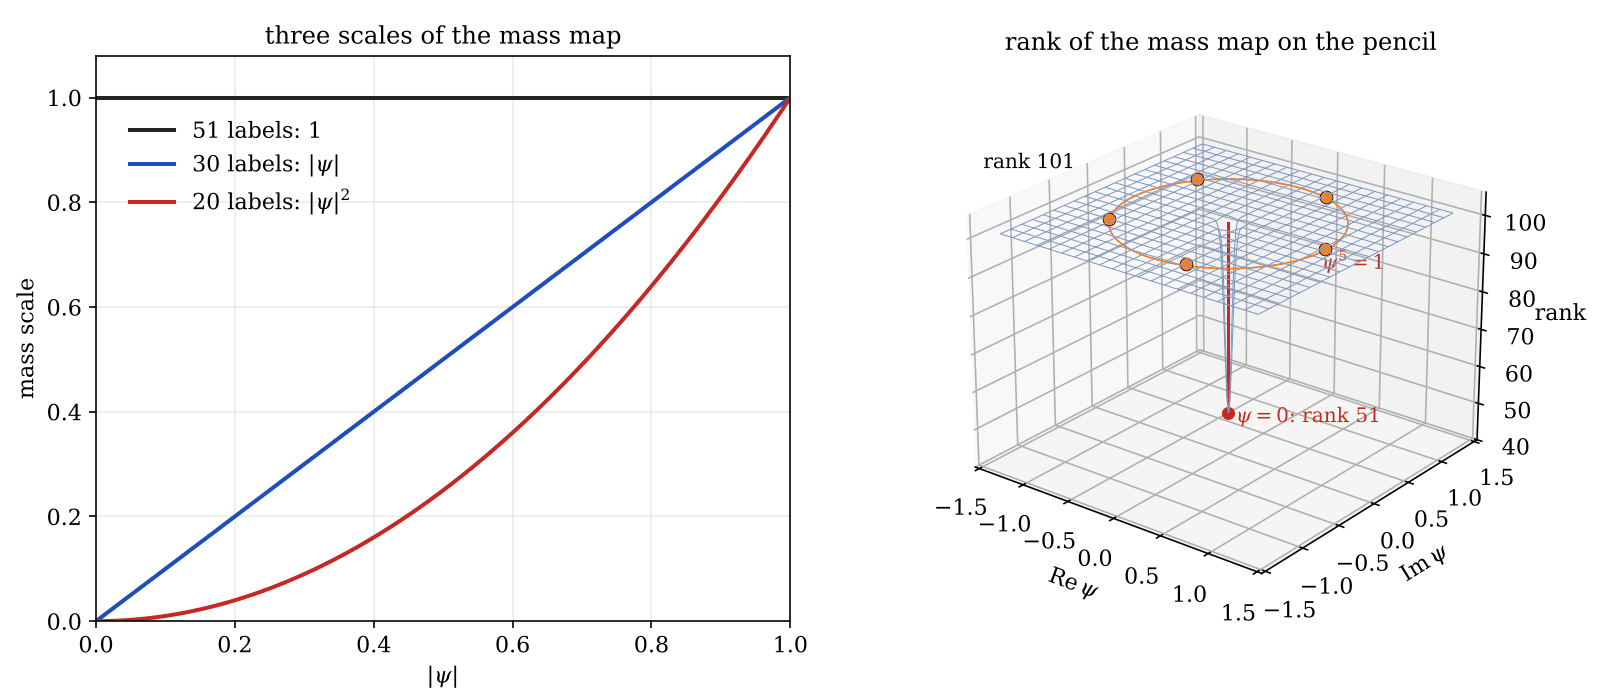
\includegraphics[width=0.96\textwidth]{figures/fig_masses.png}
\caption{The mass spectrum of Theorem~\ref{thm:C} along the pencil. Left:
the three mass scales $1$, $|\psi|$ and $|\psi|^2$ against $|\psi|$ for
$0\le|\psi|<1$, with the multiplicities of the labels (fifty-one, thirty,
twenty) that carry them; the singlet $h$ sits in the first group. Right: the
rank of the mass map over the $\psi$-plane, fifty-one at the Fermat point
and a hundred and one elsewhere (the drop at $\psi=0$ is drawn with a small
width); the conifold points $\psi^5=1$, where the Jacobian ring
degenerates, are marked on the unit circle.}
\label{fig:masses}
\end{figure}

\begin{remark}[Degenerations]
The determinant $\pm\psi^{70}$ shows that the mass map of the invariant
direction degenerates on the pencil only at the Fermat point, where the
group of automorphisms of $X_\psi$ jumps from $\Gamma\rtimes S_5$ to the
full group of order $5^4\cdot120$ of the Fermat quintic. The fifty massless
generations at $\psi=0$ are the labels with an exponent three. The larger
group acts on a monomial through its full exponent vector, not only through
its class modulo $\one$, so at $\psi=0$ a coupling of $h$, $\bb$ and $\cc$
survives only if $\one+\bb+\cc=(3,3,3,3,3)$; for a label with an exponent
three the required partner $2\one-\bb$ has a negative entry.
At the conifold points $\psi^5=1$ the matrix $M$ has nonzero determinant,
but the normalisation of Remark~\ref{rem:hessian} has a pole: the holomorphically normalized residue expression has a pole.
A statement about a physical coupling also requires its matter and
Hodge metrics; a pole of that expression alone is not a proof of
a universal physical divergence. See~\cite{CDGP91} for the period behavior.
\end{remark}

\section{The Fermat point}\label{sec:fermat}

At $\psi=0$ the Hodge norms are explicit.

\begin{proposition}[Hodge norms at the Fermat point]\label{prop:fermat}
Let $X_0$ be the Fermat quintic and $\omega_{\bb}$ the class of $x^{\bb}$,
$\bb\in B$. Write $k_i=b_i+1$ and $\gamma(t)=\Gamma(t)/\Gamma(1-t)$. There
is a constant $C>0$ independent of $\bb$ such that
\begin{equation}\label{eq:gamma}
g_{\bb}=\ip{\omega_{\bb}}{\overline{\omega_{\bb}}}=C\prod_{i=1}^5
\gamma(k_i/5).
\end{equation}
\end{proposition}

\begin{proof}
The full group $\mu_5^5/\mu_5$ of diagonal phases acts on $X_0$, and
$\omega_{\bb}$ spans the eigenline of the character $\mathbf k=(k_i)$, with
$1\le k_i\le4$ and $\sum k_i=10$. Eigenlines of distinct characters are
orthogonal for the Hodge metric, so $g_{\bb}$ is the only entry of the
metric on that line, and it is computed from the periods of $\omega_{\bb}$
by the second Riemann bilinear relation: if $P$ is an integral cycle and
$P_{\mathbf k}$ its component in the eigenspace of $\mathbf k$ in
$H_3(X_0,\C)$, then $g_{\bb}=|\int_P\omega_{\bb}|^2/
|P_{\mathbf k}\cdot P_{-\mathbf k}|$ up to a factor depending only on the
Hodge type. For the cycle of Pham, the join of the five sets of fifth roots
of unity, the period is a product of beta integrals, and the intersection
number is a product of factors $1-\zeta^{k_i}$; combining them with
$\Gamma(t)\Gamma(1-t)=\pi/\sin\pi t$ gives \eqref{eq:gamma}. This is the
computation of Candelas~\cite{Can88} on the Fermat quintic and, in the
language of the Gepner model, of Distler and Greene~\cite{DG88}; the steps
are written out in Appendix~\ref{app:fermat}.
\end{proof}

The proposition fixes the ratios of the Hodge norms inside $H^{2,1}$, which
is all that the masses of Theorem~\ref{thm:C} need. Since $\gamma(1-t)=
1/\gamma(t)$, every norm is a monomial in the two numbers
$\gamma(1/5)=3.94325$ and $\gamma(2/5)=1.48951$. For the singlet,
$\mathbf k=(2,2,2,2,2)$ and $g_{\one}=C\gamma(2/5)^5$; for the type
$\{2,1,1,1,0\}$, $\mathbf k$ is a permutation of $(3,2,2,2,1)$ and
$g_{\bb}=C\gamma(2/5)^2\gamma(1/5)$; for the type $\{2,2,1,0,0\}$,
$\mathbf k$ is a permutation of $(3,3,2,1,1)$ and $g_{\bb}=C\gamma(1/5)^2/
\gamma(2/5)$. The ratio of the second to the first is
$\Gamma(3/5)^3\Gamma(1/5)/\Gamma(2/5)^3\Gamma(4/5)=1.19324$, the square of
the constant $\kappa=1.09236$ in which Distler and Greene~\cite{DG88}
expressed the normalised couplings of the Gepner model
(see~\cite[eq.~(4.3)]{BMT24}). The norm of $\Omega$, the class of $1$ with
$\mathbf k=(1,1,1,1,1)$, has the same shape with a different constant, and
the Weil--Petersson metric of the pencil at the Fermat point, computed from
the periods by Candelas, de la Ossa, Green and Parkes~\cite{CDGP91}, is
\[
G_{\psi\bar\psi}(0)=25\,\frac{\Gamma(2/5)^5\,\Gamma(4/5)^5}
{\Gamma(1/5)^5\,\Gamma(3/5)^5}=0.19226,
\]
the value that Butbaia and collaborators~\cite{BMT24} reproduce with
numerical Ricci-flat metrics.\footnote{In~\cite{BMT24} the value is given
for the mirror quintic, whose complex structure moduli space is the
$\psi$-line of the Dwork pencil divided by the symmetry
$\psi\mapsto\zeta\psi$. The Weil--Petersson metric is
$-\partial\bar\partial\log\int\Omega\wedge\overline\Omega$, and passing to
the quotient by $\Gamma$ multiplies $\int\Omega\wedge\overline\Omega$ by the
constant $1/125$, which does not change the metric; the two numbers are
therefore the same. Their machine-learned harmonic representatives give
$0.1906$ against the exact $0.1923$.}

Inserting \eqref{eq:gamma} into Theorem~\ref{thm:C} gives the fifty-one
nonzero masses at the Fermat point. Each label of the types
$\{2,1,1,1,0\}$ and $\{2,2,1,0,0\}$ is paired with a label of the same type
and the same multiset of $k_i$, so $g_{\bb}=g_{\sigma\bb}$ and its mass is
$v/g_{\bb}$; the singlet has mass $v/g_{\one}$. Table~\ref{tab:fermat} lists
the values. In units of the singlet mass the two doublet masses are
$0.83805$ (twenty labels, ten doublets) and $0.70234$ (thirty labels,
fifteen doublets). The fifty generations with an exponent three are
massless there, and acquire masses proportional to $|\psi|$ (thirty) and
$|\psi|^2$ (twenty) as the modulus moves off the Fermat point.

\begin{table}[t]
\caption{Hodge norms and masses at the Fermat point, from
\eqref{eq:gamma} and Theorem~\ref{thm:C}. Norms are in units of $C$ and
masses in units of $v/C$; the types with an exponent three are massless at
$\psi=0$.}
\label{tab:fermat}
\centering
\begin{adjustbox}{max width=\linewidth}\begin{tabular}{lrlll}
\toprule
type & count & $g_{\bb}/C$ & value & mass\\
\midrule
$\{1,1,1,1,1\}$ & 1 & $\gamma(2/5)^5$ & $7.33179$ & $0.136392$\\
$\{2,1,1,1,0\}$ & 20 & $\gamma(2/5)^2\gamma(1/5)$ & $8.74859$ & $0.114304$\\
$\{2,2,1,0,0\}$ & 30 & $\gamma(1/5)^2/\gamma(2/5)$ & $10.4392$ & $0.095793$\\
$\{3,1,1,0,0\}$ & 30 & $\gamma(2/5)^2\gamma(1/5)$ & $8.74859$ & $0$\\
$\{3,2,0,0,0\}$ & 20 & $\gamma(1/5)^2/\gamma(2/5)$ & $10.4392$ & $0$\\
\bottomrule
\end{tabular}\end{adjustbox}
\end{table}

\section{Weighted Fermat pencils}\label{sec:weighted}

\subsection{The pencils}

In this section $(d;w)$ is one of $(6;1,1,1,1,2)$, $(8;1,1,1,1,4)$ and
$(10;1,1,1,2,5)$, so that $d=\sum w_i$ and $n_i=d/w_i$ is an integer:
$n=(6,6,6,6,3)$, $(8,8,8,8,2)$ and $(10,10,10,5,2)$. The polynomial
$F_\psi=\sum_ix_i^{n_i}-d\psi P$, $P=x_1x_2x_3x_4x_5$, is weighted
homogeneous of degree $d$ for $\deg x_i=w_i$, and $X_\psi\subset\PP(w)$ is
its zero locus \eqref{eq:wpencil}. We write
\[
\delta=\prod_iw_i^{w_i}\in\{4,\,256,\,12\,500\},
\]
and use the letters $i,j,k,l$ for distinct indices among the coordinates of
weight one. Table~\ref{tab:wdata} collects the numbers proved in this
section, with the quintic for comparison.\footnote{The three pencils are the
weighted members of the family of one-parameter models whose periods and
mirror maps were computed by Morrison~\cite{Mor92}, Klemm and
Theisen~\cite{KT93} and Font~\cite{Fon93}. In those papers the coefficient
of $P$ is normalised differently and the natural coordinate on the moduli
space is $\psi^d$ up to a constant; the discriminant $\psi^d\delta=1$ below
is the conifold locus of those papers, and the Fermat point $\psi=0$ is the
Gepner point.}

\begin{table}[t]
\caption{The four pencils of Fermat type. The rows give the degree and
weights, the constant $\delta=\prod w_i^{w_i}$ of the discriminant
$\psi^d\delta=1$, the intersection numbers of the hyperplane class $L$, the
Euler characteristic and $h^{2,1}$, the order of $\Gamma$, the number of
distinct characters carried by the generations, the number of classes of
two or three generations sharing a character, the number of characters of
$\Gamma$ carried by no generation, and the rank of the mass map of the
invariant direction for $\psi\ne0$ and at $\psi=0$, with the number of
generations it leaves massless.}
\label{tab:wdata}
\centering
\begin{adjustbox}{max width=\linewidth}\begin{tabular}{lcccc}
\toprule
 & quintic & sextic & octic & dectic\\
\midrule
$(d;w)$ & $(5;1,1,1,1,1)$ & $(6;1,1,1,1,2)$ & $(8;1,1,1,1,4)$ & $(10;1,1,1,2,5)$\\
$\delta$ & $1$ & $4$ & $256$ & $12\,500$\\
$L^3$, $c_2\cdot L$ & $5$, $50$ & $3$, $42$ & $2$, $44$ & $1$, $34$\\
$\chi$, $h^{2,1}$ & $-200$, $101$ & $-204$, $103$ & $-296$, $149$ & $-288$, $145$\\
$|\Gamma|$ & $125$ & $108$ & $128$ & $100$\\
distinct characters & $101$ & $96$ & $122$ & $100$\\
shared classes & $0$ & $7$ & $27$ & $42$\\
characters not carried & $24$ & $12$ & $6$ & $0$\\
rank for $\psi\ne0$ (massless) & $101$ ($0$) & $99$ ($4$) & $125$ ($24$) & $109$ ($36$)\\
rank at $\psi=0$ (massless) & $51$ ($50$) & $44$ ($59$) & $85$ ($64$) & $72$ ($73$)\\
\bottomrule
\end{tabular}\end{adjustbox}
\end{table}

\begin{lemma}\label{lem:wsmooth}
If $\psi^d\delta\ne1$, then $X_\psi$ is quasi-smooth, it misses the singular
points of $\PP(w)$, and it is a smooth Calabi--Yau threefold with
$h^{1,1}=1$. Its hyperplane class $L=c_1(\cO_X(1))$ generates $H^2(X,\Z)$
modulo torsion, and
\begin{equation}\label{eq:wchern}
\begin{gathered}
L^3=\frac{d}{\prod_iw_i},\qquad c_2\cdot L=\sigma_2(w)\,L^3,\\
\chi=\big(\sigma_3(w)-d\,\sigma_2(w)\big)L^3,
\end{gathered}
\end{equation}
with $\sigma_k$ the elementary symmetric functions of the weights. If
$\psi^d\delta=1$, then $X_\psi$ is singular.
\end{lemma}

\begin{proof}
The Euler relations $x_i\partial_iF_\psi=n_ix_i^{n_i}-d\psi P$ show that at a
common zero of the partial derivatives $x_i^{n_i}=w_i\psi P$ for every $i$.
If $P=0$ this forces $x=0$. Otherwise raise the $i$-th relation to the power
$w_i$ and multiply: since $\prod_ix_i^{n_iw_i}=P^d$, this gives
$P^d=\psi^d\delta P^d$, so $\psi^d\delta=1$. Hence $X_\psi$ is quasi-smooth
when $\psi^d\delta\ne1$. Conversely, at $\psi=2^{-1/3}$, $\psi=1/2$ and
$\psi=2^{-1/5}5^{-1/2}$ the points $(1,1,1,1,2^{1/3})$, $(1,1,1,1,2)$ and
$(1,1,1,2^{1/5},5^{1/2})$ satisfy $x_i^{n_i}=w_i\psi P=w_i$, so they are
singular points of the sextic, octic and dectic; the other roots of
$\psi^d\delta=1$ are $\zeta\psi$ with $\zeta^d=1$, and
$x_1\mapsto\zeta^{-1}x_1$ maps $X_{\zeta\psi}$ to $X_\psi$ because $n_1=d$.

The singular points of $\PP(w)$ are $(0{:}0{:}0{:}0{:}1)$ for the sextic
and the octic, with isotropy $\mu_2$ and $\mu_4$, and $(0{:}0{:}0{:}1{:}0)$
and $(0{:}0{:}0{:}0{:}1)$ for the dectic, with isotropy $\mu_2$ and $\mu_5$.
Each monomial $x_i^{n_i}$ occurs in $F_\psi$ with coefficient one, so $F_\psi$
does not vanish at a coordinate point and $X_\psi$ misses them all; a
quasi-smooth hypersurface in the smooth locus of $\PP(w)$ is smooth. By
adjunction $K_X=\cO_X(d-\sum w_i)=\cO_X$, and the Lefschetz theorem for
quasi-smooth hypersurfaces~\cite{Dol82} gives $h^{1,0}=h^{2,0}=0$ and
$h^{1,1}=1$.

The tangent bundle of $\PP(w)$ on its smooth locus has total Chern class
$\prod_i(1+w_iH)$ by the weighted Euler sequence, and the normal bundle of
$X$ is $\cO_X(d)$, so $c(T_X)=\prod_i(1+w_iL)(1+dL)^{-1}$. Expanding with
$\sigma_1(w)=d$ gives $c_1=0$, $c_2=\sigma_2L^2$ and
$c_3=(\sigma_3-d\sigma_2)L^3$, and $L^3=d\int_{\PP(w)}H^4=d/\prod w_i$. For
the three pencils $(\sigma_2,\sigma_3)=(14,16)$, $(22,28)$ and $(34,52)$,
which gives Table~\ref{tab:wdata}. If $L=mL'$ with $L'$ integral, then
$m^3$ divides $L^3\in\{3,2,1\}$, which is cube-free, so $m=\pm1$; as
$H^2(X,\Q)$ is spanned by $L$, the class $L$ generates $H^2(X,\Z)$ modulo
torsion.
\end{proof}

\subsection{Labels and characters}

The Jacobian ring $R=\C[x_1,\dots,x_5]/(\partial_1F_\psi,\dots,
\partial_5F_\psi)$ is graded by $\deg x_i=w_i$. Quasi-smoothness says that
the partial derivatives, of degrees $d-w_i$, form a regular sequence, so
$R$ is a graded complete intersection with Hilbert series
$\prod_i(1-t^{d-w_i})/(1-t^{w_i})$: it has dimension $\prod_i(n_i-1)$, which
is $1250$, $2401$ and $2916$, its top degree is $\sum_i(d-2w_i)=3d$, and
$R_{3d}$ is one-dimensional and spanned by $\Hess F_\psi$ by Macaulay's
theorem, which holds for any regular sequence of weighted homogeneous
polynomials. Griffiths' description of the Hodge structure extends to
quasi-smooth hypersurfaces in weighted projective space, as shown by
Steenbrink~\cite{Ste77} and Dolgachev~\cite{Dol82}: with
\[
\Omega_0=\sum_i(-1)^iw_ix_i\,dx_1\wedge\cdots\widehat{dx_i}\cdots\wedge dx_5,
\]
the residue along $X$ of $P\,\Omega_0/F_\psi^{q+1}$, for $P$ of degree
$qd$, identifies $R_{qd}$ with $H^{3-q,q}(X)$, so that $H^{2,1}=R_d$ and
$R_{3d}$ is the socle. The
infinitesimal variation of the Hodge structure is again multiplication in
$R$, and the cubic form is \eqref{eq:jacobianyukawa} with $\lambda$ a
functional on $R_{3d}$; the derivation in~\cite{CG80} uses only the residue
map and the residue pairing of $R$, both of which are available in the
weighted setting.

Let $B$ be the set of $\bb\in\Z^5$ with $0\le b_i\le n_i-2$ and
$\sum_iw_ib_i=d$. We call its elements the labels.

\begin{lemma}\label{lem:wlabels}
Let $\psi^d\delta\ne1$. Every monomial $x^{\ee}$ of degree $d$ satisfies
$x^{\ee}\equiv c\,\psi^r x^{\bb}$ in $R$ with $\bb\in B$, $c$ a product of
weights, and $r\le1$ for the sextic and $r\le2$ for the octic and the
dectic. The monomials $x^{\bb}$, $\bb\in B$, are a basis of $R_d=H^{2,1}$,
so $|B|=h^{2,1}$.
\end{lemma}

\begin{proof}
The relations $\partial_iF_\psi/n_i=0$ read
\begin{equation}\label{eq:wreduce}
x_i^{n_i-1}\equiv w_i\psi\prod_{j\ne i}x_j .
\end{equation}
In a monomial of degree $d$ at most one exponent satisfies $e_i\ge n_i-1$:
two such exponents would carry weight at least $2d-w_i-w_j>d$. If
$e_i\ge n_i-1$, then $e_i\in\{n_i-1,n_i\}$, and \eqref{eq:wreduce} replaces
$x^{\ee}$ by $w_i\psi\,x^{\ee'}$ with $e'_i=e_i-n_i+1$ and $e'_j=e_j+1$ for
$j\ne i$. If $e_i=n_i$, then $x^{\ee}=x_i^{n_i}$ and $\ee'=\one$. If
$e_i=n_i-1$, then $e'_i=0$, the other coordinates carry weight $w_i$, and
$e'_j\ge n_j-1$ forces $w_je_j\ge d-2w_j$, hence $w_i+2w_j\ge d$. For the
sextic no pair $i\ne j$ has $w_i+2w_j\ge6$, and $\one\in B$ because every
$n_j\ge3$; so one step suffices. For the octic and the dectic the only $j$
with $w_i+2w_j\ge d$ for some $i\ne j$ is $j=5$, where $w_5=d/2$ and
$n_5=2$; in that case, and in the case $\ee'=\one$, the exponent of $x_5$
is one and a second step at $x_5$ gives an exponent vector with $e''_5=0$
and the other entries raised by one. A third step would need $w_5+2w_k\ge
d$, that is $w_k\ge d/4$, for some $k\le4$, which fails. So at most two
steps reach a vector with all $e_i\le n_i-2$, which is a label.

At $\psi=0$ the ring is $\bigotimes_i\C[x_i]/(x_i^{n_i-1})$, whose
monomials with $e_i\le n_i-2$ are a basis; so $|B|=\dim R_d$. The Hilbert
series does not depend on $\psi$, and the labels span $R_d$ for every
$\psi$ by the first part, so they are a basis.
\end{proof}

\paragraph*{The symmetry group.}
Let $K$ be the group of $\varepsilon\in\prod_i\mu_{n_i}$ with
$\prod_i\varepsilon_i=1$, acting by $x_i\mapsto\varepsilon_ix_i$. It
preserves $F_\psi$ for every $\psi$. The elements
$(\lambda^{w_1},\dots,\lambda^{w_5})$ with $\lambda^d=1$ lie in $K$ and act
trivially on $\PP(w)$, and they are the only such elements; they form a
subgroup isomorphic to $\mu_d$ because the weights are coprime. Let
$\Gamma=K/\mu_d$. Since $\mathrm{lcm}(n_i)=d$, the product map
$\prod_i\mu_{n_i}\to\mu_d$ is onto and $|\Gamma|=\prod_in_i/d^2$, which is
$108$, $128$ and $100$. A character of $\prod_i\mu_{n_i}$ is a vector
$\bb\in\bigoplus_i\Z/n_i$, acting by $\varepsilon\mapsto\prod_i
\varepsilon_i^{b_i}$; it is trivial on $K$ exactly when it is a multiple of
$\one$, and it is trivial on $\mu_d$ exactly when $\sum_iw_ib_i\equiv0
\pmod d$, a condition that is well defined because $w_in_i=d$. Hence
\[
\widehat\Gamma=\Big\{\bb\in\textstyle\bigoplus_i\Z/n_i:\ \sum_iw_ib_i
\equiv0\pmod d\Big\}\Big/\langle\one\rangle .
\]
A monomial $x^{\ee}$ of degree divisible by $d$ transforms by the class
$[\ee]$ of its exponent vector, and $\Omega_0$ transforms by
$\prod_i\varepsilon_i=1$, so the isomorphisms $R_{qd}\cong H^{3-q,q}$ are
$\Gamma$-equivariant and $R$ is graded by $\widehat\Gamma$. The Hessian is
invariant, since $\partial_i\partial_jF_\psi$ transforms by
$\varepsilon_i^{-1}\varepsilon_j^{-1}$ and the determinant by
$\prod_i\varepsilon_i^{-2}=1$; so $R_{3d}$ carries the trivial character.
Permutations of coordinates of equal weight also preserve $F_\psi$ and
permute the labels.

\begin{lemma}[Wrapping]\label{lem:wwrap}
Two labels $\bb\ne\bb'$ carry the same character if and only if there is a
shift $s\in\{1,\dots,d-1\}$ such that, with $a_i=\lfloor(b_i+s)/n_i\rfloor$,
\[
\begin{gathered}
b'_i=b_i+s-n_ia_i,\qquad \sum_ia_i=s,\\
b_i+s\not\equiv n_i-1\pmod{n_i}\quad\text{for all }i .
\end{gathered}
\]
The shift from $\bb'$ back to $\bb$ is then $d-s$.
\end{lemma}

\begin{proof}
Both labels satisfy $\sum w_ib_i=d\equiv0$, so they define the same
character exactly when $\bb'\equiv\bb+s\one$ modulo $(n_1,\dots,n_5)$ for
some $s$ modulo $d$. As $0\le b'_i\le n_i-2$, the entry $b'_i$ is the
residue of $b_i+s$ in $\{0,\dots,n_i-1\}$, which must differ from $n_i-1$.
Then $\sum_iw_ib'_i=\sum_iw_ib_i+sd-d\sum_ia_i$, which equals $d$ exactly
when $\sum_ia_i=s$.
\end{proof}

\begin{proposition}\label{prop:wchars}
Let $\psi^d\delta\ne1$. The classes of labels that carry the same character
are exactly the following, and every other label carries a character of its
own.
\begin{enumerate}[label=\textup{(\alph*)},leftmargin=*,itemsep=1pt]
\item Sextic: the $4$ pairs $\{x_i^4x_5,\ x_j^2x_k^2x_l^2\}$ at shift
$2$ and the $3$ pairs $\{x_i^3x_j^3,\ x_k^3x_l^3\}$ at shift $3$; $96$
distinct characters.
\item Octic: the $12$ pairs $\{x_i^6x_j^2,\ x_j^4x_k^2x_l^2\}$ and the $12$
pairs $\{x_i^6x_jx_k,\ x_j^3x_k^3x_l^2\}$ at shift $2$, and the $3$ pairs
$\{x_i^4x_j^4,\ x_k^4x_l^4\}$ at shift $4$; $122$ distinct characters.
\item Dectic: the three triples $\{x_i^8x_4,\,x_j^2x_k^2x_4^3,\,
x_i^2x_j^4x_k^4\}$; at shift $2$ the $12$ pairs $\{x_1^{c_1}x_2^{c_2}
x_3^{c_3}x_4^3,\allowbreak\ x_1^{c_1+2}x_2^{c_2+2}x_3^{c_3+2}\}$ with $c_1+c_2+c_3=4$
and $\cc$ not a permutation of $(2,2,0)$, the $6$ pairs
$\{x_i^8x_j^2,\allowbreak\ x_j^4x_k^2x_4^2\}$ and the $3$ pairs
$\{x_i^8x_jx_k,\allowbreak\ x_j^3x_k^3x_4^2\}$; at shift $4$ the $6$ pairs
$\{x_i^6x_j^2x_4,\allowbreak\ x_j^6x_k^4\}$, the $3$ pairs
$\{x_i^6x_jx_kx_4,\allowbreak\ x_j^5x_k^5\}$, the $6$ pairs
$\{x_i^7x_jx_4,\allowbreak\ x_ix_j^5x_k^4\}$ and the $3$ pairs
$\{x_i^6x_4^2,\allowbreak\ x_j^4x_k^4x_4\}$; $100$ distinct characters, so every
character of $\Gamma$ is carried by some generation.
\end{enumerate}
The characters carried by no label are the $12$ classes of
$(\pi(0,1,3,4),2)$ for the sextic and the $6$ classes of
$(\pi(0,2,4,6),1)$ for the octic, $\pi$ running over the permutations of
four entries. The set of characters carried by labels is closed under
$\chi\mapsto-\chi$.
\end{proposition}

\begin{proof}
We use Lemma~\ref{lem:wwrap} and treat the shifts $s\le d/2$; the others
are their inverses. For the sextic, $b_i+s\le9<12$ for $i\le4$, so
$a_i=1$ exactly when $b_i\ge6-s$, and the residue $n_i-1=5$ is excluded
when $b_i=5-s$; for $x_5$, $b_5\le1$ and $a_5=\lfloor(b_5+s)/3\rfloor$,
with $b_5+s\equiv2\pmod3$ excluded. At $s=1$ we have $a_5=0$ and need one
$b_i\ge5$, which is impossible. At $s=2$ the value $b_5=0$ is excluded, so
$b_5=1$ and $a_5=1$; we need exactly one $b_i\ge4$ among the first four,
which sum to four, so $\bb=(4,0,0,0,1)$ up to order, and its image is
$(0,2,2,2,0)$. At $s=3$ we have $a_5=1$ and need two entries $b_i\ge3$
among the first four and none equal to two; two entries of at least three
already have weight six, so $\bb=(3,3,0,0,0)$ up to order, with image
$(0,0,3,3,0)$. No label occurs at two different shifts, so the classes are
the pairs listed, $14$ labels in $7$ classes and $103-7=96$ characters.
The same analysis for the octic and the dectic is carried out in
Appendix~\ref{app:wlabels}. It uses two facts: for these pencils $n_5=2$
and $b_5=0$, so $a_5=s/2$ and an odd shift is excluded by the residue of
$x_5$; and the bounds $b_i\le n_i-2$ make each $a_i$ either $0$ or $1$,
except $a_4\in\{0,1,2\}$ for the dectic.

The characters not carried by a label are $108-96=12$, $128-122=6$ and
$100-100=0$ in number. For the sextic, adding $s\one$ to
$(\pi(0,1,3,4),2)$ gives a vector with an entry $5$ for $s\not\equiv0
\pmod3$, and the vector $(\pi'(0,1,3,4),2)$ for $s=3$, where the last entry
is $n_5-1$. So every representative of these classes has an entry $n_i-1$,
and none is a label; each class contains two of the $24$ vectors
$(\pi(0,1,3,4),2)$, which gives $12$ classes, and these are all the missing
characters. For the octic, adding $s\one$ to $(\pi(0,2,4,6),1)$ gives an
entry $7$ when $s$ is odd and the last entry $1=n_5-1$ when $s$ is even;
each class contains four of the $24$ vectors, which gives $6$ classes.
Finally $-(\pi(0,1,3,4),2)=(\pi(0,5,3,2),1)$, which becomes
$(\pi(1,0,4,3),2)$ after adding $\one$, and $-(\pi(0,2,4,6),1)=
(\pi(0,6,4,2),1)$; so the missing characters are closed under negation,
and so are the carried ones.
\end{proof}

Figure~\ref{fig:weighted} compares the four pencils.

\begin{figure}[t]
\centering
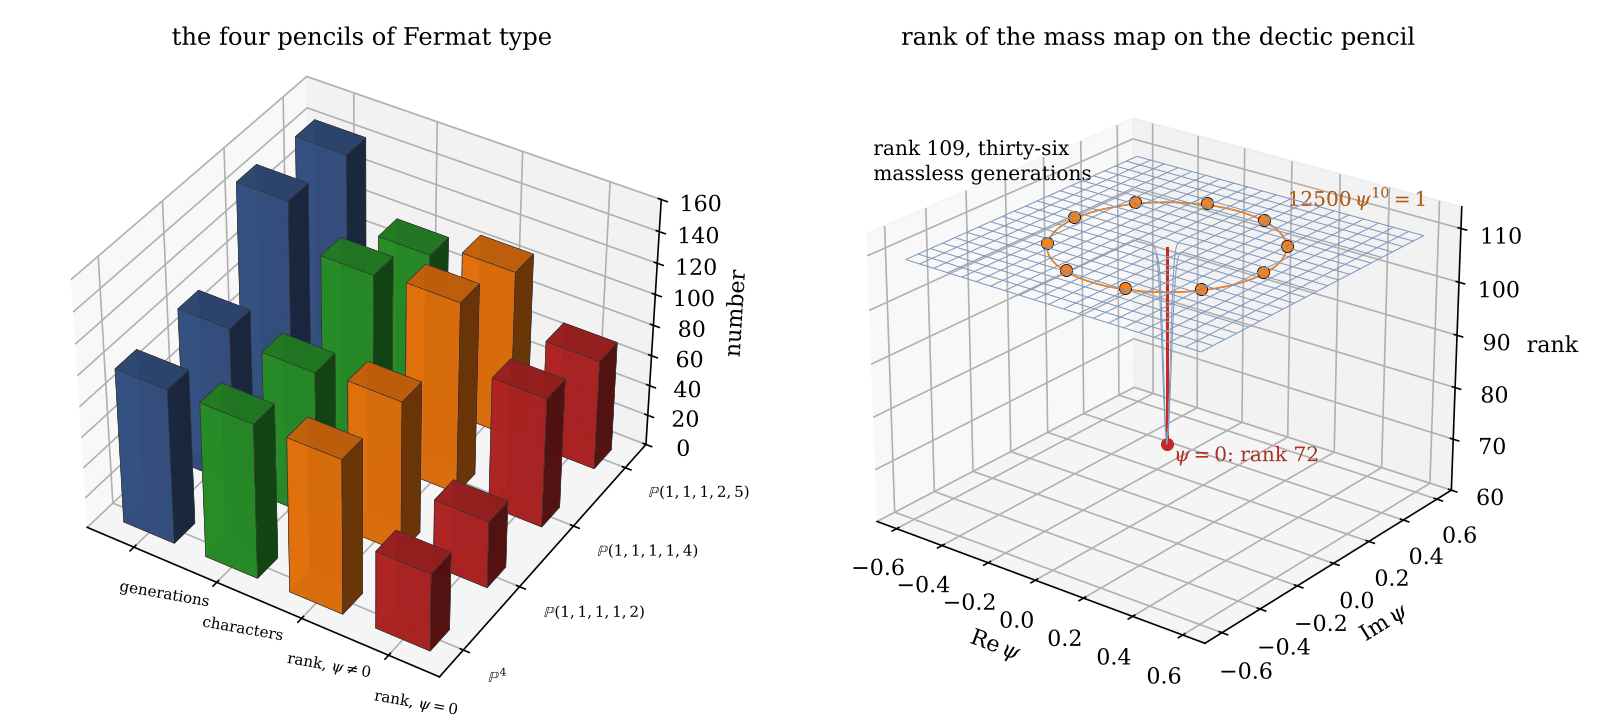
\includegraphics[width=0.96\textwidth]{figures/fig_weighted.png}
\caption{Left: for the quintic in $\PP^4$ and the sextic, octic and dectic
pencils in $\PP(1,1,1,1,2)$, $\PP(1,1,1,1,4)$ and $\PP(1,1,1,2,5)$, the
number of generations ($101$, $103$, $149$, $145$), the number of distinct
characters they carry ($101$, $96$, $122$, $100$), and the rank of the mass
map of the invariant direction for $\psi\ne0$ ($101$, $99$, $125$, $109$)
and at $\psi=0$ ($51$, $44$, $85$, $72$). Only on the quintic do the first
three bars agree. Right: the rank of the mass map over the $\psi$-plane of
the dectic pencil, $109$ off the Fermat point and $72$ at $\psi=0$ (the drop
is drawn with a small width); the ten points of the circle
$12\,500\,\psi^{10}=1$ are the singular members.}
\label{fig:weighted}
\end{figure}

\subsection{The socle functional}

Let $m_0=x^{\mathbf n-2\one}$, the monomial with exponents $n_i-2$; it has
degree $\sum_iw_i(n_i-2)=3d$. A monomial $x^{\ee}$ of degree $3d$ is in
sector $r\in\{0,\dots,d-1\}$ if $e_i\equiv n_i-2-r\pmod{n_i}$ for every
$i$. We then write
\begin{equation}\label{eq:wsector}
e_i=n_i-2-r+n_ik_i ;
\end{equation}
each $k_i$ is a nonnegative integer, since $k_i\le-1$ would give
$e_i\le-2-r$, and $\sum_ik_i=r$, by comparing degrees:
$\sum_iw_ie_i=5d-2d-rd+d\sum_ik_i=3d$.

\begin{theorem}[Weighted socle functional]\label{thm:wsocle}
Let $\psi^d\delta\ne1$. Then $m_0$ spans $R_{3d}$, and the functional
$\lambda$ on $R_{3d}$ with $\lambda(m_0)=1$ satisfies, for every monomial
$x^{\ee}$ of degree $3d$,
\[
\lambda(x^{\ee})=\begin{cases}\psi^r\prod_iw_i^{k_i}&\text{if $\ee$ is in
sector $r$, with $k$ as in \eqref{eq:wsector},}\\
0&\text{otherwise.}\end{cases}
\]
A monomial of degree $3d$ is in a sector if and only if its character is
trivial.
\end{theorem}

\begin{proof}
The character of $x^{\ee}$ is trivial when $\ee\equiv c\one$ modulo
$(n_1,\dots,n_5)$ for some integer $c$; taking $r\equiv-2-c\pmod d$ and
using $n_i\mid d$ this is the condition $e_i\equiv n_i-2-r$, so the
monomials with trivial character are those in a sector. Since $R_{3d}$ is
one-dimensional with trivial character, every monomial with a nontrivial
character vanishes in $R$.

Let $\ee$ be in sector $r\ge1$. We claim that some $i$ has $n_ik_i\ge
r+1$. Otherwise $k_i\le r/n_i=rw_i/d$ for every $i$, so $r=\sum_ik_i\le
r\sum_iw_i/d=r$, with equality only if $n_ik_i=r$ for every $i$; then every
$n_i$ divides $r$, and so does their least common multiple $d$, which is
impossible for $1\le r<d$. For such an $i$ we have $e_i\ge n_i-1$, and
\eqref{eq:wreduce} gives $x^{\ee}\equiv w_i\psi\,x^{\ee'}$ with
$e'_i=e_i-n_i+1$ and $e'_j=e_j+1$ for $j\ne i$; by \eqref{eq:wsector}
$\ee'$ is in sector $r-1$ with $k'_i=k_i-1$ and the other $k_j$ unchanged.
After $r$ steps we reach sector $0$, where all $k_i$ vanish and
$\ee=\mathbf n-2\one$. Collecting the factors,
$x^{\ee}\equiv\psi^r\prod_iw_i^{k_i}\,m_0$. Finally, $R_{3d}$ is spanned
by monomials, each of which is zero or a multiple of $m_0$, and
$R_{3d}\ne0$; so $m_0$ spans $R_{3d}$.
\end{proof}

\begin{corollary}\label{cor:wcouplings}
Let $\psi^d\delta\ne1$. The cubic form takes on three labels
$\va,\bb,\cc$ the value $\lambda(x^{\va+\bb+\cc})$, up to the normalisation
of $\lambda$: this is $\psi^r\prod_iw_i^{k_i}$ when $\va+\bb+\cc$ is in
sector $r$, and zero when the character of $x^{\va+\bb+\cc}$ is
nontrivial. In particular, for $\psi\ne0$ every coupling allowed by
$\Gamma$ is nonzero. This is Theorem~\ref{thm:E}(ii).
\end{corollary}

\subsection{The mass map}

The only label with trivial character is $h=\one$ for the sextic and
$h=(2,2,2,2,0)$ for the octic and the dectic: a label $\bb\equiv c\one$ has
$b_i=c$ for the coordinates of weight one, and the condition on the weight
leaves only these. So the invariant part of $R_d$ is spanned by $x^h$,
the invariant direction. For $\psi\ne0$ it contains the tangent vector
$\partial_\psi F_\psi=-dP$ of the pencil: for the sextic $P=x^h$, and for
the octic and the dectic $P=x^{\one}\equiv w_5\psi\,x^h$ by
\eqref{eq:wreduce} at $x_5$, whose exponent one equals $n_5-1$. By
Corollary~\ref{cor:wcouplings} the mass map of the invariant direction in
the basis of labels is
\[
M_{\bb\cc}=\lambda\big(x^{h+\bb+\cc}\big),\qquad \bb,\cc\in B .
\]
Since $h$ has trivial character, $M_{\bb\cc}\ne0$ requires
$[\cc]=-[\bb]$. For a character $\chi$ let $B_\chi$ be the set of labels
carrying it; then $M$ is the direct sum of the blocks on
$B_\chi\cup B_{-\chi}$, one for each pair $\{\chi,-\chi\}$ of characters
carried by labels (Proposition~\ref{prop:wchars} shows that $-\chi$ is
carried whenever $\chi$ is).

\begin{lemma}\label{lem:wminor}
Let $\psi\ne0$ and $\psi^d\delta\ne1$. Every entry of a block is
$\psi^r\prod_iw_i^{k_i}\ne0$. For $\bb,\bb'\in B_\chi$ and
$\cc,\cc'\in B_{-\chi}$ let $r$, $r'$, $\rho$, $\rho'$ be the sectors of
$h+\bb+\cc$, $h+\bb'+\cc'$, $h+\bb+\cc'$ and $h+\bb'+\cc$, and
$\Delta=r+r'-\rho-\rho'$. Then $\Delta\in\{-d,0,d\}$, and
\[
\begin{aligned}
&M_{\bb\cc}M_{\bb'\cc'}-M_{\bb\cc'}M_{\bb'\cc}\\
&\qquad=M_{\bb\cc'}M_{\bb'\cc}\big((\psi^d\delta)^{\Delta/d}-1\big),
\end{aligned}
\]
which vanishes exactly when $\Delta=0$.
\end{lemma}

\begin{proof}
The first statement is Theorem~\ref{thm:wsocle}, since each
$h+\bb+\cc$ in a block has trivial character. The two sums
$(h+\bb+\cc)+(h+\bb'+\cc')$ and $(h+\bb+\cc')+(h+\bb'+\cc)$ are equal, so
by \eqref{eq:wsector}, with $k,k',\kappa,\kappa'$ the vectors of the four
monomials, $n_i(k_i+k'_i-\kappa_i-\kappa'_i)=\Delta$ for every $i$. Hence
every $n_i$ divides $\Delta$, so $d$ does, and $|\Delta|<2d$ because the
sectors lie in $\{0,\dots,d-1\}$. The quotient of the two products is
$\psi^{\Delta}\prod_iw_i^{\Delta w_i/d}=(\psi^d\delta)^{\Delta/d}$.
\end{proof}

\begin{table}[t]
\caption{The blocks of the mass map of the invariant direction that
involve labels sharing a character. Each row gives the labels of
$B_\chi$ and of $B_{-\chi}$ in the notation of
Proposition~\ref{prop:wchars} (one representative of the orbit under
permutations of the coordinates of weight one), the number of such blocks,
the entries $M_{\bb\cc}$ with $\bb\in B_\chi$ in the order listed, and the
number of generations each block leaves massless for $\psi\ne0$; ``self''
means $-\chi=\chi$. All other blocks are a single label with $\chi=-\chi$
or a pair of single labels, and have full rank.}
\label{tab:wblocks}
\centering
\begin{adjustbox}{max width=\linewidth}\begin{tabular}{llllrr}
\toprule
pencil & $B_\chi$ & $B_{-\chi}$ & entries & blocks & massless\\
\midrule
sextic & $x_i^4x_5,\ x_j^2x_k^2x_l^2$ & $x_i^3x_jx_kx_l$ &
$2\psi^2;\ 1$ & $4$ & $1$\\
 & $x_i^3x_j^3,\ x_k^3x_l^3$ & self & $(2\psi^3,1;\ 1,2\psi^3)$ & $3$ & $0$\\
\midrule
octic & $x_i^6x_jx_k,\ x_j^3x_k^3x_l^2$ & $x_i^4x_jx_kx_l^2$ &
$4\psi^2;\ 1$ & $12$ & $1$\\
 & $x_i^6x_j^2,\ x_j^4x_k^2x_l^2$ & $x_j^6x_i^2,\ x_i^4x_k^2x_l^2$ &
$(16\psi^4,4\psi^2;\ 4\psi^2,1)$ & $6$ & $2$\\
 & $x_i^4x_j^4,\ x_k^4x_l^4$ & self & $(16\psi^4,1;\ 1,16\psi^4)$ & $3$ & $0$\\
\midrule
dectic & $x_i^2x_jx_kx_4^3,\ x_i^4x_j^3x_k^3$ & $x_i^2x_j^3x_k^3x_4$ &
$10\psi^2;\ 1$ & $3$ & $1$\\
 & $x_i^3x_jx_4^3,\ x_i^5x_j^3x_k^2$ & $x_ix_j^3x_k^4x_4$ &
$10\psi^2;\ 1$ & $6$ & $1$\\
 & $x_i^8x_jx_k,\ x_j^3x_k^3x_4^2$ & $x_i^4x_jx_kx_4^2$ &
$50\psi^4;\ 10\psi^2$ & $3$ & $1$\\
 & $x_i^7x_jx_4,\ x_ix_j^5x_k^4$ & $x_i^5x_jx_k^2x_4$ &
$50\psi^4;\ 1$ & $6$ & $1$\\
 & $x_i^8x_4,\ x_j^2x_k^2x_4^3,\ x_i^2x_j^4x_k^4$ & $x_i^4x_j^2x_k^2x_4$ &
$50\psi^4;\ 10\psi^2;\ 1$ & $3$ & $2$\\
 & $x_i^4x_4^3,\ x_i^6x_j^2x_k^2$ & $x_i^6x_4^2,\ x_j^4x_k^4x_4$ &
$(500\psi^6,10\psi^2;\ 50\psi^4,1)$ & $3$ & $2$\\
 & $x_i^8x_j^2,\ x_j^4x_k^2x_4^2$ & $x_j^8x_i^2,\ x_i^4x_k^2x_4^2$ &
$(250\psi^6,50\psi^4;\ 50\psi^4,10\psi^2)$ & $3$ & $2$\\
 & $x_i^6x_j^2x_4,\ x_j^6x_k^4$ & $x_i^6x_k^2x_4,\ x_k^6x_j^4$ &
$(50\psi^4,1;\ 1,250\psi^6)$ & $3$ & $0$\\
 & $x_i^6x_jx_kx_4,\ x_j^5x_k^5$ & self & $(50\psi^4,1;\ 1,250\psi^6)$ & $3$ & $0$\\
\bottomrule
\end{tabular}\end{adjustbox}
\end{table}

\begin{proposition}\label{prop:wmass}
Let $\psi\ne0$ and $\psi^d\delta\ne1$. The blocks of the mass map that
involve labels sharing a character are those of Table~\ref{tab:wblocks}.
The mass map has rank $99$, $125$ and $109$ for the sextic, octic and
dectic, its kernel has dimension $4$, $24$ and $36$ and lies in the span of
the labels that share a character, and the rank is the same at every member
with $\psi\ne0$ and $\psi^d\delta\ne1$. At $\psi=0$ the mass map is the
matrix of the partial involution $\bb\mapsto\mathbf n-2\one-h-\bb$ on the
labels with $\bb\le\mathbf n-2\one-h$, of rank $44$, $85$ and $72$.
\end{proposition}

\begin{proof}
The classes of Proposition~\ref{prop:wchars} and their negatives give the
rows of Table~\ref{tab:wblocks}: for one representative of each orbit the
character $-\chi$ is computed from Lemma~\ref{lem:wwrap}, and the entries
from Theorem~\ref{thm:wsocle}; Appendix~\ref{app:wblocks} lists the sectors
and the vectors $k$. For example, for the sextic block with $i=1$,
$h+(3,1,1,1,0)+(4,0,0,0,1)=(8,2,2,2,2)$ is in sector $2$ with
$k=(1,0,0,0,1)$, which gives $2\psi^2$, and $h+(3,1,1,1,0)+(0,2,2,2,0)=
(4,4,4,4,1)=\mathbf n-2\one$ gives $1$. A block in which one of $B_\chi$,
$B_{-\chi}$ is a single label has the form $\left(\begin{smallmatrix}0&A\\
A^{\mathsf T}&0\end{smallmatrix}\right)$ with $A$ a row or a column of
nonzero entries, so it has rank two and leaves $|B_\chi|+|B_{-\chi}|-2$
generations massless, in the span of the class of two or three labels. For
a block with $2\times2$ matrix $A$, Lemma~\ref{lem:wminor} decides the
rank: $\Delta=0$ for the second octic row and the sixth and seventh dectic
rows, for instance $6+0-2-4=0$ in the sixth, so $A$ has rank one and two
generations on each side of the block are massless; $\Delta=\pm d$ for the
eighth dectic row and the three self-dual rows, whose determinants are
$4\psi^6-1$, $256\psi^8-1$ and $12\,500\psi^{10}-1$ up to nonzero
monomials, so these blocks have full rank. A single label with
$\chi=-\chi$, and a pair of single labels, give a block of full rank by the
first part of Lemma~\ref{lem:wminor}. Adding the last column of
Table~\ref{tab:wblocks}: $4\cdot1=4$, $12\cdot1+6\cdot2=24$ and
$3+6+3+6+3\cdot2+3\cdot2+3\cdot2=36$. None of the entries or
determinants depends on $\psi$ beyond these monomials and the factor
$\psi^d\delta-1$, so the rank is constant on the stated set.

At $\psi=0$ every sector $r\ge1$ gives zero, so $M_{\bb\cc}\ne0$ exactly
when $h+\bb+\cc=\mathbf n-2\one$. The vector
$\cc=\mathbf n-2\one-h-\bb$ has degree $3d-2d=d$ and entries at most
$n_i-2$, so it is a label exactly when $\bb\le\mathbf n-2\one-h$. Here
$\mathbf n-2\one-h=(3,3,3,3,0)$, $(4,4,4,4,0)$ and $(6,6,6,1,0)$, and the
labels below these vectors are counted by the coefficient of $t^6$ in
$(1+t+t^2+t^3)^4$, which is $44$, of $t^8$ in $(1+t+\dots+t^4)^4$, which is
$85$, and by $36+36=72$ solutions of $b_1+b_2+b_3+2b_4=10$ with $b_i\le6$
and $b_4\le1$.
\end{proof}

\subsection{Three families}

\begin{proposition}\label{prop:wthree}
Let $X$ be a member of the sextic, octic or dectic pencil with
$\psi^d\delta\ne1$, and $H$ a finite group acting freely on $X$. With the
standard embedding, $X/H$ does not have three net families.
\end{proposition}

\begin{proof}
By Theorem~\ref{thm:dictionary} the number of net families on $Y=X/H$ is
$|\chi(Y)|/2=|\chi(X)|/(2|H|)$, and three families need
$|H|=|\chi(X)|/6$, that is $34$ for the sextic and $48$ for the dectic; for
the octic $296/6$ is not an integer. Suppose $H$ has this order. The
projection $\pi\colon X\to Y$ is \'etale of degree $|H|$, $\chi(\cO_Y)=
\chi(\cO_X)/|H|=0$ and $c_1(Y)$ is torsion. As $H^2(X,\Q)=\Q L$ and $L$
generates $H^2(X,\Z)$ modulo torsion (Lemma~\ref{lem:wsmooth}), every line
bundle $D$ on $Y$ has $\pi^*D\equiv mL$ numerically for an integer $m$, and
these $m$ form a subgroup of $\Z$. It contains $|H|$: the line bundle
$\bigotimes_{g\in H}g^*\cO_X(1)$ is linearised by permuting its factors, so
it descends to $Y$, and it is numerically $|H|L$ because $H$ acts trivially
on $H^2(X,\Q)$. Let $m_0>0$ generate the subgroup and $D$ realise it. Then
$m_0$ divides $|H|$, and
\[
\begin{gathered}
D^3=\frac{m_0^3L^3}{|H|},\qquad c_2(Y)\cdot D=\frac{m_0\,c_2\cdot L}{|H|},\\
\chi(Y,D)=\frac{D^3}{6}+\frac{c_2(Y)\cdot D}{12},
\end{gathered}
\]
the last by Riemann--Roch with $c_1(Y)\equiv0$ and $\chi(\cO_Y)=0$. All
three numbers are integers. For the sextic, $D^3=3m_0^3/34$ forces
$34\mid m_0$, so $m_0=34$, $D^3=3468$, $c_2(Y)\cdot D=42$ and
$\chi(Y,D)=578+7/2$. For the dectic, $D^3=m_0^3/48$ forces $12\mid m_0$ and
$c_2(Y)\cdot D=17m_0/24$ forces $24\mid m_0$, so $m_0\in\{24,48\}$, with
$\chi(Y,D)=48+17/12$ and $384+17/6$. None is an integer, a contradiction.
\end{proof}

\begin{proof}[Proof of Theorem~\ref{thm:E}]
Smoothness and $h^{2,1}$ are Lemma~\ref{lem:wsmooth}, part (i) is
Proposition~\ref{prop:wchars}, part (ii) is
Corollary~\ref{cor:wcouplings}, part (iii) is Proposition~\ref{prop:wmass},
and part (iv) is Proposition~\ref{prop:wthree} together with
$|\chi(X)|/2\in\{102,148,144\}$ for $X$ itself.
\end{proof}

\begin{remark}[Why the quintic is different]\label{rem:wquintic}
On the quintic all $n_i$ equal five, so a shift moves every exponent by the
same amount and the wrapping count $\sum_ia_i=s$ of
Lemma~\ref{lem:wwrap} has no solution: this is the proof of
Theorem~\ref{thm:A}. When the $n_i$ differ, a wrap at a coordinate with
large $n_i$ can be balanced by wraps at the coordinate with $n_5=3$ or
$n_5=2$, and the shared classes of Proposition~\ref{prop:wchars} are
exactly these balances. The mass map then has blocks larger than $1\times1$
whose entries, all nonzero, satisfy $\Delta=0$, and these blocks carry the
massless generations. Among the four pencils, the quintic is therefore the
only one on which the characters of the symmetry group label the
generations and the invariant deformation gives every generation a mass.
\end{remark}



\section{The simultaneous construction problem}\label{sec:selection}
The GSC formulation in \cite{Dwork,Mirror} concerns a landscape
$\mathcal L=\coprod_\tau M_\tau$ of compactification data and an involutive
isometry $\mu$ defined on a union $D$ of components. A desired function
$S:\mathcal L\to[0,\infty)$ is smooth and proper on each component,
has a unique global minimum at a viable point, and is invariant under
$\mu$ wherever $\mu$ is defined. Its viability requirements originate in
\cite{Original}. We use the following short restatement, without supplying
new numerical meanings for the physical acceptance conditions.

\begin{center}\small
\begin{adjustbox}{max width=\linewidth}\begin{tabular}{@{}p{.07\linewidth}p{.85\linewidth}@{}}
\toprule
C1 & A slope-polystable bundle with $c_1=0$ and an effective anomaly class.\\
C2 & Three net families, with the quotient index treated consistently.\\
C3 & Wilson-line reduction of the visible gauge group to the Standard Model.\\
C4 & Three quark--lepton families and no chiral exotics after projection.\\
C5 & Allowed sufficiently heavy masses for vectorlike exotics.\\
C6 & A Higgs pair with doublet--triplet splitting.\\
C7 & Stabilization of the relevant moduli in a controlled effective regime.\\
C8 & Acceptable physical Yukawa rank and hierarchy after normalization.\\
C9 & Phenomenologically consistent supersymmetry breaking, if present.\\
\bottomrule
\end{tabular}\end{adjustbox}
\end{center}

These are nine simultaneous predicates on one complete datum, not nine
alternative cases. Let $A_i$ be the locus satisfying C$i$. The existence
problem is $\bigcap_{i=1}^9 A_i\ne\varnothing$. Nonemptiness of separate
$A_i$, even of all pairs among three loci, need not imply a common point:
$\{0,1\}$, $\{1,2\}$ and $\{0,2\}$ have pairwise intersections but empty
triple intersection. Results at different bundles or different moduli
values cannot be assembled into a single vacuum without proving their
compatibility.

For a complete datum one must specify the threefold, visible and hidden
bundles, polarization, free action and equivariant structures when used,
Wilson line, effective K\"ahler potential and superpotential, and the
domain in which omitted corrections are controlled. C5 and C7--C9 also
need explicit acceptance predicates. Without them the conjecture is not a
mathematical statement, since a threshold ``fixed by comparison with
measurement'' is not a predicate on a datum. We fix one choice. The
numbers are conventions, and a different choice gives a different
conjecture; the failures proved in this paper for C7 and C8 hold for every
choice, as Remark~\ref{rem:windowsrobust} records.

\begin{definition}[The acceptance windows $W$]\label{def:windows}
A datum satisfies the three conditions with the windows $W$ when:
\begin{enumerate}[label=\textup{C\arabic*$_W$},start=7,leftmargin=*,itemsep=2pt]
\item at the vacuum every modulus, that is every K\"ahler, complex
structure, bundle and dilaton field of the four-dimensional theory, has a
canonically normalized mass of at least $m_0=3\times10^4$ GeV; no exactly
flat direction is allowed. The value is the lower bound for moduli that
decay before nucleosynthesis \cite{BKN94,AKK12}.
\item at the scale $\mu=2\times10^{16}$ GeV the up-type, down-type and
charged-lepton Yukawa matrices have rank three, and their singular-value
ratios lie within a factor three of the values
\begin{gather*}
 \frac{m_u}{m_t}=5.3\times10^{-6},\qquad \frac{m_c}{m_t}=2.6\times10^{-3},\qquad
 \frac{m_d}{m_b}=8.9\times10^{-4},\\
 \frac{m_s}{m_b}=1.6\times10^{-2},\qquad
 \frac{m_e}{m_\tau}=2.8\times10^{-4},\qquad \frac{m_\mu}{m_\tau}=5.9\times10^{-2},
\end{gather*}
the ratios of the running masses at that scale in the minimal
supersymmetric standard model with $\tan\beta=10$ \cite[Table~V]{XZZ08};
the Cabibbo element satisfies $0.15\le|V_{us}|\le0.30$. The factor three
covers the dependence on $\tan\beta$ between the two cases tabulated in
\cite{XZZ08} and the threshold corrections at the matching scales.
\item supersymmetry is broken, some F-term being nonzero at the vacuum,
and the gravitino mass lies in $[10^3,10^6]$ GeV, the window around $m_0$
in which gravity-mediated soft masses lie between the weak scale and the
moduli scale \cite{AKK12}.
\end{enumerate}
\end{definition}

\begin{conjecture}[GSC$(W)$]\label{conj:gscw}
There is a complete datum, in the sense of the list above, satisfying
C1--C6 and C7$_W$--C9$_W$.
\end{conjecture}

\begin{remark}[Dependence on the windows]\label{rem:windowsrobust}
Only a positive certificate depends on $W$. The negative results of this
paper do not: a flat direction of the classical potential, as on the
volume ray of the fixed datum in Section~\ref{sec:pointfailure}, violates
C7$_W$ for every $m_0>0$; a Yukawa matrix of rank at most two, or a
vanishing one, violates C8$_W$ for every window around any nonzero ratios;
and the selection rules of Proposition~\ref{prop:eleven} are statements
about vanishing matrices. Where the paper writes C7, C8 or C9 below, the
conditions are those of Definition~\ref{def:windows}.
\end{remark}

\section{A marked-point selection construction}
The functional conditions have a clean differential-topological answer.
They do not manufacture the point that is to be selected.

\begin{theorem}[Selection with a supplied point]\label{thm:selection}
Let $M$ be a countable disjoint union of second-countable smooth
Riemannian manifolds. Let $\mu$ be an involutive isometry on a union $D$
of components. Given $p\in M$, the following are equivalent:
\begin{enumerate}[label=(\roman*)]
\item $p\notin D$, or $\mu p=p$.
\item There is a nonnegative smooth globally proper function $S$ on $M$
with unique zero $p$ and $S\circ\mu=S$ on $D$.
\end{enumerate}
The function can be chosen to have Hessian $2g_p$ at $p$.
\end{theorem}
\begin{proof}
An invariant function with unique zero must fix that zero under every
symmetry defined there. This proves necessity.

Every second-countable smooth manifold has a nonnegative smooth proper
exhaustion $\rho$. One direct construction takes a compact exhaustion
$K_j\subset\operatorname{int}K_{j+1}$, a locally finite partition of unity
subordinate to the compact annular cover, and assigns successively increasing
positive coefficients to its terms; outside $K_j$ all nonzero coefficients
can be arranged to be at least $j$. Its sublevel sets are closed and
contained in some $K_j$, hence compact. These standard smooth-manifold
constructions apply separately to the components; see \cite{Lee}.

On a component preserved by $\mu$, replace $\rho$ by
$\rho+\rho\circ\mu$. On a pair of exchanged components choose $\rho$ on
one and transport it to the other. The resulting function is invariant
and proper on each component. Enumerate the component orbits; outside
the orbit of the component of $p$, add distinct positive integer offsets
tending to infinity. Each orbit contains at most two components.

Choose a normal ball $B_r(p)$ with compact closure, and write
$f(x)=d(p,x)^2$ there. If $p\in D$ and is fixed, this ball and $f$ are
invariant. Choose a smooth function $\theta:[0,\infty)\to[0,1]$ equal to
one for $t\le r^2/4$ and zero for $t\ge r^2/2$. On the component of $p$ set
\[
 S=\theta(f)f+(1-\theta(f))(1+\rho),
\]
extending the expression by $1+\rho$ outside the ball. This is smooth
because $\theta(f)$ vanishes near its boundary. Its only zero is $p$:
away from $p$ every nonzero term in this convex combination is positive.
It equals $f$ near $p$, so its Hessian there is $2g_p$.

On the remaining components use their exhaustion plus the positive
orbit offset. For a fixed sublevel only finitely many offsets occur.
On the distinguished component a sublevel is a closed subset of
$\overline B_r(p)\cup\{\rho\le t-1\}$; on all other relevant components
it is compact by properness of $\rho$. Thus every sublevel of $S$ is
compact in the disjoint union. Invariance follows from the construction.
\end{proof}

\begin{remark}[What the point supplies]
The construction uses the marked point $p$, exhaustions and cutoffs in
addition to the metric. It proves the smooth-function assertion with a
supplied compatible point. It does not prove that an unmarked metric
determines $p$ or that $p$ satisfies C1--C9.
\end{remark}

\begin{proposition}[An intrinsic selector must respect all isometries]
Suppose a rule assigns $S_g$ to an unmarked Riemannian manifold naturally
under isometries. If $S_g$ has a unique minimum $p$, every isometry fixes
$p$. In particular there is no such uniquely minimizing rule on a
positive-dimensional homogeneous Riemannian manifold.
\end{proposition}
\begin{proof}
Naturality for an isometry $h$ says $S_g(hx)=S_g(x)$. Hence $hp$ is
another minimum and equals $p$. Transitivity on a manifold with more
than one point is incompatible with a common fixed point.
\end{proof}
This is an obstruction to a particular notion of metric-only selection,
not a proof that the actual heterotic moduli metric is homogeneous.
It also shows why invariance under an additional compact group cannot be
discarded merely because the partial mirror map is undefined at $p$:
the additional group must still fix a unique selected point.

\section{Index constraints and the mirror restriction}
\begin{proposition}[Index and finite descent]\label{prop:index}
Let $X$ be a Calabi--Yau threefold and $V$ a holomorphic bundle with
$c_1(V)=0$. Then
\[
 \chi(X,V)=\frac12\int_Xc_3(V).
\]
If $\pi:X\to Y$ is finite \emph{\'etale} of degree $d$ and
$V=\pi^*V_Y$, then $\chi(X,V)=d\chi(Y,V_Y)$. Thus the three-family
index condition downstairs requires $|\int_Xc_3(V)|=6d$.
\end{proposition}
\begin{proof}
In Hirzebruch--Riemann--Roch, the degree-six term of
$\operatorname{ch}(V)\operatorname{td}(X)$ is
$\operatorname{ch}_3(V)+c_1(V)c_2(X)/12+\operatorname{rk}(V)c_1(X)c_2(X)/24$.
The last two terms vanish and $\operatorname{ch}_3(V)=c_3(V)/2$.
For an \emph{\'etale} map the tangent bundle and Todd class pull back,
and integration of a pulled-back top class multiplies by $d$.
\end{proof}

For a quintic, expansion of $(1+H)^5/(1+5H)$ gives
$c_3(T_X)=-40H^3$ and $\int_XH^3=5$, hence $\int c_3(T_X)=-200$.
Consequently no standard-embedding
free quotient has index of absolute value three, because $100=3d$ has no
integer solution. This restriction is independent of the quotient group
classification. It does not apply to arbitrary nonstandard bundles.

Under the standard-type partial mirror convention of \cite{Mirror}, a
fixed point has $h^{1,1}=h^{2,1}$ and hence $\chi(X)=0$. The bundle on
that component has $\int c_3(V)=\chi(X)$, so Proposition~\ref{prop:index}
gives zero net families. This proves that a selected viable point cannot
be a mirror-fixed point in that specified domain. It does not exclude
nonstandard data outside the domain, nor establish a mirror map on all
$(0,2)$ compactifications.



\subsection{The Dwork pencil}

\begin{proposition}\label{prop:dworkselect}
\textup{(i)} For $\psi\ne0$ and $\psi^5\ne1$, the mass map of the invariant
direction $h$ on $X_\psi$ has rank $101$, its entries in the basis of
labels are $1$, $\psi$ and $\psi^2$, on $51$, $30$ and $20$ labels, and the
masses of Theorem~\ref{thm:C} are $|\psi|^{r(\bb)}$ times the Hodge factor
$(g_{\bb}g_{\sigma\bb})^{-1/2}$.

\textup{(ii)} Let $X$ be a smooth quintic threefold and $H$ a finite group
acting freely on $X$. The standard embedding on $X/H$ has
$100/|H|$ net families. In particular condition \textup{(C2)} fails on
$X/H$ for every such $H$, and no vacuum of the form $(X/H,T_{X/H})$ is
viable.

\textup{(iii)} On the sextic, octic and dectic pencils of
Section~\ref{sec:weighted}, with $\psi\ne0$ and $\psi^d\delta\ne1$, the
mass map of the invariant direction has a kernel of dimension $4$, $24$ and
$36$, and condition \textup{(C2)} fails on every member and on every
quotient of a member by a group acting freely.
\end{proposition}

\begin{proof}
Part (i) is Theorem~\ref{thm:C}. For (ii), a smooth quintic has
$h^{1,1}=1$ and $h^{2,1}=101$, so $\chi(X)=-200$. A free action multiplies
the Euler characteristic of the quotient by $1/|H|$, so
$\chi(X/H)=-200/|H|$, and by Theorem~\ref{thm:dictionary} the net number of
families is $|\chi(X/H)|/2=100/|H|$. Wilson lines on $X/H$ break the gauge
group but do not change this index. The equation $100/|H|=3$ has no
solution in integers, so (C2) fails. Part (iii) is
Propositions~\ref{prop:wmass} and~\ref{prop:wthree}.
\end{proof}

\section{Free quotients of the one-parameter families}\label{sec:freequot}

The four pencils are four of the fourteen one-parameter families of
Calabi--Yau threefolds with $h^{1,1}=1$ whose Picard--Fuchs equations are
hypergeometric, listed by Doran and Morgan~\cite{DM06}. Thirteen of them are
complete intersections $X=X_{d_1,\dots,d_c}\subset\PP(w)$ of degrees
$d_1,\dots,d_c$ with $\sum_jd_j=\sum_iw_i$, whose general member is
quasi-smooth and misses the singular points of $\PP(w)$; they are the rows
of Table~\ref{tab:freequot}. The fourteenth, $X_{2,12}\subset
\PP(1,1,1,1,4,6)$, is not of this kind: its quadric involves only the four
coordinates of weight one, so it is not quasi-smooth at the point of
$\PP(4,6)$ where the equation of degree twelve vanishes, and we leave it
aside. For the thirteen, the count of families of
Proposition~\ref{prop:dworkselect} becomes a statement about every free
quotient, through one arithmetic invariant.

\begin{lemma}[Primes of a free action]\label{lem:freeprime}
Let $X$ be a compact K\"ahler threefold with $K_X\cong\cO_X$,
$h^{1,0}=h^{2,0}=0$, $b_2=1$ and $\pi_1(X)=0$, let $L$ be an ample line
bundle on $X$, and let $g$ be an automorphism of prime order $p$ without
fixed points. Then $p$ divides $\chi(X,kL)$ for every $k\ge1$.
\end{lemma}

\begin{proof}
Since $X$ is simply connected, $H^2(X,\Z)$ has no torsion, and since
$h^{0,1}=h^{0,2}=0$ the first Chern class identifies $\operatorname{Pic}X$
with $H^2(X,\Z)\cong\Z$. Let $A$ be its ample generator, so that $L=A^a$
with $a\ge1$. The bundle $g^*A$ is again an ample generator, so
$g^*A\cong A$. The obstruction to lifting the action of the cyclic group
$G=\langle g\rangle$ to $A$ lies in $H^2(G,\C^*)$, which vanishes for a
cyclic group, so $A$ and all its powers are $G$-linearised and $G$ acts on
$H^q(X,A^m)$. For $m\ge1$ these groups vanish in positive degree by
Kodaira's theorem, as $A^m=K_X\otimes A^m$ with $A^m$ ample. For $1\le
j<p$ the automorphism $g^j$ has no fixed points, and the holomorphic
Lefschetz formula of Atiyah and Bott~\cite{AB68} gives
$\sum_q(-1)^q\operatorname{tr}\big(g^j\,|\,H^q(X,A^m)\big)=0$, that is,
$\operatorname{tr}(g^j\,|\,H^0(X,A^m))=0$. A representation of $\Z/p$ whose
character vanishes off the identity is a multiple of the regular
representation, so $p$ divides $h^0(X,A^m)=\chi(X,A^m)$. Taking $m=ka$
gives the statement.
\end{proof}

\begin{table}[t]
\caption{The thirteen one-parameter complete intersections. The columns
give the type, the weights, the intersection numbers, the Euler
characteristic, the values $\chi(X,kL)=k^3L^3/6+k\,c_2\cdot L/12$ for
$k=1,2,3$, their greatest common divisor $g_X$, and the order $|\chi|/6$
that a free action giving three families would need.}
\label{tab:freequot}
\centering
\begin{adjustbox}{max width=\linewidth}\begin{tabular}{llrrrlrl}
\toprule
type & $w$ & $L^3$ & $c_2\cdot L$ & $\chi$ & $\chi(kL)$ & $g_X$ & $|\chi|/6$\\
\midrule
$X_5$ & $1^5$ & $5$ & $50$ & $-200$ & $5,15,35$ & $5$ & --\\
$X_6$ & $1^4,2$ & $3$ & $42$ & $-204$ & $4,11,24$ & $1$ & $34$\\
$X_8$ & $1^4,4$ & $2$ & $44$ & $-296$ & $4,10,20$ & $2$ & --\\
$X_{10}$ & $1^3,2,5$ & $1$ & $34$ & $-288$ & $3,7,13$ & $1$ & $48$\\
$X_{3,3}$ & $1^6$ & $9$ & $54$ & $-144$ & $6,21,54$ & $3$ & $24$\\
$X_{4,2}$ & $1^6$ & $8$ & $56$ & $-176$ & $6,20,50$ & $2$ & --\\
$X_{3,2,2}$ & $1^7$ & $12$ & $60$ & $-144$ & $7,26,69$ & $1$ & $24$\\
$X_{2,2,2,2}$ & $1^8$ & $16$ & $64$ & $-128$ & $8,32,88$ & $8$ & --\\
$X_{4,4}$ & $1^4,2^2$ & $4$ & $40$ & $-144$ & $4,12,28$ & $4$ & $24$\\
$X_{6,6}$ & $1^2,2^2,3^2$ & $1$ & $22$ & $-120$ & $2,5,10$ & $1$ & $20$\\
$X_{4,3}$ & $1^5,2$ & $6$ & $48$ & $-156$ & $5,16,39$ & $1$ & $26$\\
$X_{6,4}$ & $1^3,2^2,3$ & $2$ & $32$ & $-156$ & $3,8,17$ & $1$ & $26$\\
$X_{6,2}$ & $1^5,3$ & $4$ & $52$ & $-256$ & $5,14,31$ & $1$ & --\\
\bottomrule
\end{tabular}\end{adjustbox}
\end{table}

\begin{proposition}\label{prop:freequot}
Let $X\subset\PP(w)$ be a quasi-smooth complete intersection of one of the
thirteen types of Table~\ref{tab:freequot} that misses the singular points
of $\PP(w)$, and let $H$ be a finite group acting freely on $X$. Then every
prime divisor of $|H|$ divides $g_X$. Hence $H$ is trivial for $X_6$,
$X_{10}$, $X_{3,2,2}$, $X_{6,6}$, $X_{4,3}$, $X_{6,4}$ and $X_{6,2}$; it is
a $5$-group for $X_5$, a $3$-group for $X_{3,3}$, and a $2$-group for
$X_8$, $X_{4,2}$, $X_{2,2,2,2}$ and $X_{4,4}$. With the standard embedding,
no free quotient of $X$ carries three net families.
\end{proposition}

\begin{proof}
As in Lemma~\ref{lem:wsmooth}, $X$ is a smooth threefold with $K_X\cong
\cO_X(\sum_jd_j-\sum_iw_i)=\cO_X$, and the Lefschetz theorem for
quasi-smooth complete intersections~\cite{Dol82} gives $h^{1,0}=h^{2,0}=0$
and $b_2=1$. For $\pi_1$, let $C\subset\C^{N}$ be the affine cone over $X$,
the zero set of the $c$ weighted homogeneous equations. Quasi-smoothness
says that $C$ is a complete intersection of dimension four with an isolated
singular point at the origin, so by Hamm's theorem~\cite{Ham71} its link
is $2$-connected; the weighted action of $\R_{>0}$ meets every sphere about
the origin once, so $C\setminus\{0\}$ is homotopy equivalent to the link and
is simply connected. As $X$ misses the points with nontrivial isotropy,
$\C^*$ acts freely on $C\setminus\{0\}$ with quotient $X$, and the exact
sequence of homotopy groups of this fibration gives $\pi_1(X)=0$.

Let $p$ be a prime divisor of $|H|$ and $g\in H$ an element of order $p$.
It has no fixed points, so by Lemma~\ref{lem:freeprime} with
$L=\cO_X(1)$, $p$ divides $\chi(X,kL)$ for all $k\ge1$. By Riemann--Roch,
with $c_1(X)=0$ and $\chi(\cO_X)=0$,
$\chi(X,kL)=k^3L^3/6+k\,c_2\cdot L/12$, a polynomial that takes integer
values and vanishes at $k=0$; writing it as $\alpha_1\binom k1+\alpha_2
\binom k2+\alpha_3\binom k3$ with integers $\alpha_i$, its values at all
$k\ge1$ have the same greatest common divisor as $\alpha_1,\alpha_2,
\alpha_3$, which is that of its values at $k=1,2,3$, the number $g_X$. The
intersection numbers are computed as in Lemma~\ref{lem:wsmooth}, from
$c(T_X)=\prod_i(1+w_iL)\prod_j(1+d_jL)^{-1}$ and
$L^3=\prod_jd_j/\prod_iw_i$, and give the table.

By Theorem~\ref{thm:dictionary} the quotient $X/H$ carries
$|\chi(X)|/(2|H|)$ net families, so three families need
$|H|=|\chi(X)|/6$. This is not an integer for $X_5$, $X_8$, $X_{4,2}$,
$X_{2,2,2,2}$ and $X_{6,2}$. In the remaining eight rows it is $34$, $48$,
$24$, $24$, $24$, $20$, $26$ or $26$, and each of these has a prime factor
not dividing $g_X$: $17$, $2$, $2$, $2$, $3$, $2$ and $2$ (twice).
\end{proof}

The proposition contains Theorem~\ref{thm:E}(iv) and
Proposition~\ref{prop:dworkselect}(ii) and strengthens them: the sextic and
dectic pencils admit no free action at all, and on a quintic every free
action is by a $5$-group, so that only the orders $5$ and $25$ divide
$|\chi|=200$ and a free quotient of a quintic has $20$ or $4$ families;
the quotient by $\Z/5\times\Z/5$ with four families is already
in~\cite{CHSW85}. For the five complete intersections in ordinary
projective space the free actions were classified by Braun~\cite{Bra11}
with a computer search; the proposition uses only the holomorphic
Lefschetz formula and Riemann--Roch.\footnote{On a quintic the group
$\Z/5\times\Z/5$ of~\cite{CHSW85}, generated by the cyclic permutation of
the coordinates and the diagonal phases $(1,\zeta,\zeta^2,\zeta^3,\zeta^4)$,
acts on the five coordinates through a central extension of order $125$,
the Heisenberg group, and $H^0(X,\cO_X(1))=\C^5$ is its irreducible
representation of dimension five; each cyclic subgroup of order five acts on
it by the regular representation, as Lemma~\ref{lem:freeprime} requires.}



\section{One fixed nonstandard threefold}\label{sec:fixed}
We now replace a generic existence assertion by a single specified
complex structure. The line-bundle data are the example of Buchbinder,
Constantin and Lukas \cite[Section~5.1]{BCL}; neither the bundle nor its
phenomenological interpretation is claimed here as a new discovery.
The purpose of fixing the equation is to make every subsequent calculation
refer to the same geometric datum.

In $A=(\PP^1)^4$, use coordinates $[x_i:y_i]$, $1\le i\le4$.
For $S\subset\{1,2,3,4\}$ put
\[
 m_S=\prod_{i\in S}y_i^2\prod_{i\notin S}x_i^2,
 \qquad (c_0,c_1,c_2,c_3,c_4)=(1,2,5,2,1),
 \qquad F_0=\sum_S c_{|S|}m_S.
\]
Write $r_i=x_i y_i$ and $e_i=x_i^2+y_i^2$. In the order
$(12),(13),(14),(23),(24),(34)$ let
$(a_{ij})=(1,2,3,5,7,11)$, and define
\begin{equation}\label{eq:fixedpencil}
 G=\sum_{i<j}a_{ij}r_i r_j e_k e_l+13r_1r_2r_3r_4,
 \qquad F_\theta=F_0+\theta G,
 \quad X=X_\pi=\{F_\pi=0\},
\end{equation}
where $\{k,l\}$ is the complement of $\{i,j\}$.
Here $\pi$ is the usual transcendental real number, not a freely varying
modulus. This is one projective complex threefold with completely specified
coefficients. We use transcendence only to avoid the finitely many
algebraic bad parameters of a rational pencil; it supplies no dynamical
mechanism selecting this complex structure.

\begin{lemma}[Smooth seed]\label{lem:smoothseed}
The hypersurface $F_0=0$ is smooth over $\C$.
\end{lemma}
\begin{proof}
On a coordinate stratum set the remaining nonzero affine coordinates
$t_i=y_i/x_i$ and $u_i=t_i^2$. If exactly $k$ coordinates are fixed at
infinity and $4-k-r$ at zero, the restricted polynomial is
\[
 f_{k,r}(u)=\sum_{j=0}^r c_{k+j}e_j(u_1,\ldots,u_r),
 \qquad 0\le k,\quad k+r\le4,
\]
with $e_j$ the elementary symmetric polynomial. At a singular point the
restricted polynomial and all its derivatives in the $r$ free variables
vanish. Indeed $\partial/\partial t_i=2t_i\partial/\partial u_i$ and
$t_i\ne0$. It suffices to exclude an affine singularity of each $f_{k,r}$,
even allowing zero values for its free variables.

For $r=0$ the constant is nonzero. For $r=1$ its linear coefficient is
nonzero. For $r=2$, the three determinants
$c_kc_{k+2}-c_{k+1}^2$ are $1,-21,1$, so the bilinear polynomials have
no singular zero.

For $r=3,k=0$, subtraction of two partial derivatives gives
$(u_j-u_i)(5+2u_l)$. If two coordinates differ, the third is $-5/2$,
and the partial derivative in one of the differing coordinates is
$-21/2$, a contradiction. Hence all three coordinates equal $s$.
For $r=3,k=1$ the same argument uses $(u_j-u_i)(2+u_l)$;
the forced value $-2$ makes another partial derivative equal to $1$.
The two diagonal polynomials are
\[
 q_{0,3}=1+6s+15s^2+2s^3,\qquad
 q_{1,3}=2+15s+6s^2+s^3.
\]
Both are relatively prime to their derivatives, as the explicit
B\'ezout identities in Appendix~\ref{app:certificates} show.

For $r=4$ write $f=f_{0,4}$ and
$Q(x,y)=5+2(x+y)+xy=(x+2)(y+2)+1$. Direct differentiation gives
\[
 f_i-f_j=(u_j-u_i)Q(u_k,u_l).
\]
Classify the multiplicities of four coordinates. If all are equal,
the polynomial is $q_{0,4}=1+8s+30s^2+8s^3+s^4$, again coprime to
its derivative. For multiplicities $(3,1)$, say $(x,x,x,y)$ with
$x\ne y$, the equations force $Q(x,x)=x^2+4x+5=0$.
A derivative in a repeated coordinate is $2+10x+2x^2+yQ(x,x)$,
which reduces to $2(x-4)$ modulo $Q(x,x)$. It cannot vanish since
$Q(4,4)=37$.

For multiplicities $(2,1,1)$ the equations force
$Q(x,x)=Q(x,z)=0$ with $x\ne z$. Their difference gives
$(x-z)(x+2)=0$, impossible since $Q(-2,-2)=1$. If all coordinates
are distinct, $Q(x,y)=Q(x,z)=0$ forces $x=-2$ and then $Q(x,y)=1$,
also impossible.

For multiplicities $(2,2)$, say $(x,x,y,y)$ with $x\ne y$, we have
$Q(x,y)=0$, so $y\ne-2$ and $x=-(2y+5)/(y+2)$.
After substitution, one partial derivative and $f$ have respective
numerators
\[
 g=y^2-8y-21,\qquad h=y^4-16y^3-66y^2-16y+89.
\]
Their denominators are $y+2$ and $(y+2)^2$.
The B\'ezout identity in Appendix~\ref{app:certificates} proves they
cannot both vanish. These cases exhaust the strata and partitions.
\end{proof}

Let $a$ act in all four factors by $[x:y]\mapsto[x:-y]$, and let $b$
act by $[x:y]\mapsto[y:x]$. They commute in $\operatorname{PGL}_2$ and
generate $\Gamma\cong(\Z/2)^2$. Both $F_0$ and $G$ are invariant.

\begin{theorem}[The fixed quotient]\label{thm:fixedquotient}
The threefold $X_\pi$ is smooth and $\Gamma$ acts freely, preserving its
holomorphic three-form. Thus $Y=X_\pi/\Gamma$ is a smooth projective
Calabi--Yau threefold. Its Euler characteristic is $-32$, and its
Hodge numbers are $(h^{1,1},h^{2,1})=(4,20)$.
\end{theorem}
\begin{proof}
The locus of singular fibres of the projective pencil
\eqref{eq:fixedpencil} is a closed algebraic subset of the parameter line,
defined over $\Q$: project the closed relative singular locus from
$A\times\mathbb A^1$ using properness. It omits zero by
Lemma~\ref{lem:smoothseed}, so it is finite and all its points are
algebraic over $\Q$. Transcendence of $\pi$ therefore proves smoothness
at the specified parameter, without a numerical sampling assertion.

Each of $a,b,ab$ has sixteen ambient fixed points. They have coordinates
respectively in $\{0,\infty\}$, $\{1,-1\}$ and $\{i,-i\}$ in each
factor. At these points $F_0$ is respectively one of $1,2,5$, or $48$,
or $16$, after the indicated homogeneous normalizations. All are nonzero.
The values of $G$ there are algebraic. Thus $F_0+\pi G$ is nonzero as
well, either because $G=0$ or because otherwise its vanishing would make
$\pi$ algebraic. Hence the action is free.

Adjunction gives $K_X=\cO_X$. Either generator has determinant $-1$
on each of four coordinate pairs, with product $1$. Since the defining
polynomial is invariant, the residue holomorphic three-form is invariant
and descends. Lefschetz and descent give $h^{1,0}(Y)=h^{2,0}(Y)=0$.
The ambient Chern formula gives $c_3(T_X)=-16\sum_{i<j<k}J_iJ_jJ_k$,
whose integral is $-128$;
division by four gives $\chi(Y)=-32$. The four ambient hyperplane
classes generate $H^2(X,\Q)$ and are invariant, so $h^{1,1}(Y)=4$;
$\chi(Y)=2(h^{1,1}-h^{2,1})$ then gives $h^{2,1}(Y)=20$.
\end{proof}

\section{The bundle, its spectrum and the fixed Wilson line}\label{sec:fixedbundle}
On this $X$ take $V=\bigoplus_{a=1}^5 L_a$, with $L_a=\cO_X(k_a)$
and columns
\begin{equation}\label{eq:bundle}
 K=(k_a^i)=\begin{pmatrix}
 -1&-1&0&1&1\\0&-3&1&1&1\\0&2&-1&-1&0\\1&2&0&-1&-2
 \end{pmatrix}.
\end{equation}
Fix the K\"ahler class to be $J=100(J_1+J_2+J_3+J_4)$.
The number $100$ fixes a scale in chosen units; it is not a proved
error bound for string corrections. Use the untwisted tensor lifts
of $a,b$ on all summands and zero bundle-deformation and charged-singlet
expectation values. These choices remain fixed in the audit below.

\begin{proposition}[Chern classes and slopes]\label{prop:cover}
The bundle has $c_1(V)=0$, is slope-polystable at $J$, and has
\[
 \left(\int_X c_2(V)J_i\right)=(24,8,20,12),\quad
 \int_Xc_3(V)=-24,\quad\chi(X,V)=-12.
\]
The cover anomaly class is the effective class $6J_1J_3+2J_1J_4$.
The bundle descends to $V_Y$ on $Y$, with $\chi(Y,V_Y)=-3$.
\end{proposition}
\begin{proof}
In the ambient ring $J_i^2=0$, the hypersurface class is $2\sum_iJ_i$.
Consequently $\int_XJ_iJ_jJ_k=2$ for distinct indices and zero otherwise,
and $c_2(T_X)=4\sum_{i<j}J_iJ_j$, pairing to $24$ with each $J_i$.
The rows and columns of \eqref{eq:bundle} sum to zero. Thus $c_1(V)=0$
and every summand has slope $12\cdot100^2\sum_i k_a^i=0$.
Line bundles are slope-stable; their equal-slope sum is polystable.
For $l_a=\sum_i k_a^iJ_i$ use
$c_2(V)=-\tfrac12\sum_a l_a^2$ and $c_3(V)=\tfrac13\sum_a l_a^3$.
Alternatively the line-bundle indices
\[
 \chi(\cO_X(k))=2\sum_{i<j<l}k_i k_j k_l+2\sum_i k_i
\]
are $0,-8,0,0,-4$. These give the stated numbers.
The anomaly pairs as $(0,16,4,12)$, as does $6J_1J_3+2J_1J_4$.
Lefschetz and Poincar\'e duality identify $H^4(X,\Z)$ with the integral
dual of the ambient $H^2$ basis, so these equal pairings identify the
classes. The indicated intersections of distinct hyperplane divisors
are effective.

The lifts of $a,b$ anticommute on each $\cO(1)$ factor. On
$\cO(k_a)$ their commutator is $(-1)^{\sum_i k_a^i}=1$; their squares
are one. These are commuting equivariant structures. Their product
determinant on $V$ is trivial since $\sum_a k_a=0$. The invariant
polarization descends as a real K\"ahler class, and polystability descends.
Finite \emph{\'etale} descent gives $\chi(Y,V_Y)=\chi(X,V)/4=-3$.
\end{proof}

Effectiveness of the anomaly on the cover proves rational effectiveness
downstairs by pushforward and division by four. It does not by itself
certify a quantized hidden sector or the integral torsion part of the
anomaly on $Y$. Neither has been supplied here. This qualification is
part of C1, not a correction to the proved three-family index C2.

\subsection{An exact cohomology calculation}
Let $R_\Gamma$ denote the regular representation and let $\mathbf1$
be the trivial character. A character is specified by its values on
$(a,b)$, ordered $(++),(+-),(-+),(--)$.

\begin{theorem}[Cohomology at the specified complex structure]\label{thm:fixedcohom}
For the fixed choices above,
\[
 H^1(X,V)=3R_\Gamma,\quad H^2(X,V)=0,
\]
\[
 H^1(X,\Lambda^2V)=3R_\Gamma+(R_\Gamma-\mathbf1),\qquad
 H^2(X,\Lambda^2V)=R_\Gamma-\mathbf1.
\]
Here $R_\Gamma-\mathbf1$ is the actual sum of the three nontrivial
characters. The only nonzero individual dimensions are
\begin{gather*}
 h^1(L_2)=8,\qquad h^1(L_5)=4,\\
 h^1(L_2L_4)=4,\qquad h^1(L_4L_5)=8,\\
 h^1(L_2L_5)=h^2(L_2L_5)=3.
\end{gather*}
\end{theorem}
\begin{proof}
For any multidegree $k$, use the equivariant Koszul sequence
\[
 0\longrightarrow\cO_A(k-\mathbf2)
 \xrightarrow{F_\pi}\cO_A(k)\longrightarrow\cO_X(k)\longrightarrow0.
\]
On $\PP^1$, $H^0(\cO(d))$ has dimension $d+1$ for $d\ge0$;
$H^1(\cO(d))$ has dimension $-d-1$ for $d\le-2$; all cohomology
vanishes for $d=-1$. K\"unneth therefore leaves at most one nonzero
ambient degree for each $k$.
For $L_2$, the source has $H^2$ of dimension $8$ and the target
vanishes; for $L_5$, the target has $H^1$ of dimension $4$ and the
source vanishes. The other three summands are acyclic.
For $L_2L_4$ the target has $H^1$ of dimension $4$, source zero;
for $L_4L_5$ the source has $H^2$ of dimension $8$, target zero.
For $L_2L_5=\cO_X(0,-2,2,0)$ the target has $H^1$ of dimension $3$
and the source has $H^3$ of dimension $3$, giving the two groups shown.
Six other pair products are acyclic without a rank calculation.

The remaining product is $L_1L_2=\cO_X(-2,-3,2,3)$. Both ambient
groups are $H^2$ of dimension $24$, and the relevant multiplication
matrix is $M(\theta)=M_0+\theta M_G$. In monomial bases described in
Appendix~\ref{app:certificates}, exact integer arithmetic gives
\begin{equation}\label{eq:detcertificate}
 \det M(1)=393460125696\ne0.
\end{equation}
This is a certificate that $\det M(\theta)\in\Z[\theta]$ is nonzero.
Since $\pi$ is transcendental, $M(\pi)$ is invertible. Hence $L_1L_2$
is acyclic. No assertion that $X_1$ is smooth is needed for this
determinant argument.

The character calculation is equally explicit. On a factor represent
$H^0(\cO(d))$ by $x^{d-v}y^v$, $0\le v\le d$, and
$H^1(\cO(d))$ by the \v Cech Laurent monomials with
$d+1\le v\le-1$. The generator $a$ multiplies the monomial by $(-1)^v$;
$b$ sends $v$ to $d-v$, with a minus sign for an $H^1$ factor from
interchanging the two \v Cech charts. Tensor these rules.
The groups of dimensions $8,4,4,8$ above give respectively
$2R_\Gamma,R_\Gamma,R_\Gamma,2R_\Gamma$.
Both groups for $L_2L_5$ have character multiplicities $(0,1,1,1)$.
The multiplication matrix is equivariant, so its isomorphism contributes
no further kernel or cokernel characters. This proves every asserted
representation, not just its Euler characteristic.
\end{proof}

\subsection{Projection of the charged matter}
Fix
\[
 \rho(a)=\operatorname{diag}(1,1,1,-1,-1)\in SU(5),\qquad\rho(b)=I.
\]
The centralizer inside $SU(5)$ is $S(U(3)\times U(2))$.
Taking $\Gamma$ invariants after tensoring with the Wilson representation,
each component of the three regular representations occurs three times.
The extra $R_\Gamma-\mathbf1$ in $H^1(\Lambda^2V)$ contributes one
weak doublet and no color triplet: doublets carry character $(-,+)$
and triplets $(+,+)$. Its dual in $H^2$ contributes the conjugate
doublet and no triplet. The perturbative observable charged spectrum
is therefore three $10+\overline5$ families and one Higgs doublet pair,
with no additional massless charged exotics. In this spectrum the
mass requirement for additional vectorlike charged exotics has no fields
to which it must be applied. This is a spectrum calculation, not a
calculation of singlet masses, hidden matter or Higgs potential parameters.

\subsection{A residual gauge factor at this same point}\label{sec:extraU1}
The preceding centralizer computation concerns only the $SU(5)$ factor.
The split structure group $S(U(1)^5)$ has four associated visible Abelian
gauge fields. For the standard axionic mass map at the Abelian locus,
the charges are the columns of $K$. This matrix has rank $3$, and
\begin{equation}\label{eq:extrau1}
 q=(-4,1,6,-4,1),\qquad Kq=0,\qquad\sum_aq_a=0.
\end{equation}
Thus one traceless Abelian combination is not removed by that map.
A universal-axion row of the form $\beta_i k_a^i$ also annihilates $q$.
With our zero charged-singlet expectation values there is no Higgs
mechanism removing it. Its charges on the families are $1$ on the $10$'s
from $L_2,L_5$ and $-3$ on the $\overline5$'s from $L_2L_4,L_4L_5$;
the Higgs charges are $\pm2$. These are nonzero charges, so this is not
a redundant generator. In the specified perturbative model, C3 interpreted
as precisely the Standard Model visible group therefore fails.

\section{The Yukawa and stabilization tests at that point}\label{sec:pointfailure}
This section keeps \eqref{eq:fixedpencil}, \eqref{eq:bundle}, $J$, the
Wilson line and all singlet expectation values fixed. In particular we
do not import a different model's successful flavour fit.

\begin{proposition}[A perturbative rank obstruction]\label{prop:rankfailure}
At the split-bundle point, the renormalizable perturbative up-type
Yukawa matrix has rank at most $2$, and the down-type matrix is zero.
These statements hold after any invertible matter normalization.
\end{proposition}
\begin{proof}
Let $e_a$ be the standard basis of the five charge coordinates, modulo
the common diagonal. There are two $10$ families of charge $e_2$ and
one of charge $e_5$. The up-type Higgs has charge $-e_2-e_5$.
Consequently its allowed up-type couplings have the form
\[
 Y_u=\begin{pmatrix}0&0&A\\0&0&B\\A&B&0\end{pmatrix},
\]
which has rank at most two regardless of the values of $A,B$.
The $\overline5$ families have charges $e_2+e_4$ or $e_4+e_5$,
and the down-type Higgs has charge $e_2+e_5$. Every proposed
$10\,\overline5\,H_d$ coupling therefore has total charge with first
and third components zero, nonnegative other components and total
sum five. It cannot be a multiple of $(1,1,1,1,1)$; it is forbidden
by the perturbative $S(U(1)^5)$ selection rule. Massive Abelian gauge
fields still impose this perturbative selection rule. Hence $Y_d=0$.
Invertible left and right normalization preserves rank.
\end{proof}
Nonzero singlet expectation values, a non-Abelian bundle deformation,
or computed nonperturbative contributions could change these matrices.
None is part of the fixed point just audited. Their possible existence
cannot turn its rank-deficient matrices into a verified C8 certificate.

For a leading-order unfluxed Calabi--Yau description, take vanishing
classical superpotential on the holomorphic locus and vanishing charged
expectation values. The slopes remain zero along
$J=\lambda\sum_iJ_i$ for every $\lambda>0$. Thus its D-term potential
vanishes on that ray and its F-term potential also vanishes when $W=0$.
The overall volume is a flat direction. Under the requirement that the
relevant moduli be stabilized, C7 fails in this specified approximation.
There is also no verified supersymmetry-breaking sector: the classical
F and D auxiliary fields vanish there. This cannot certify C9 if
nonzero supersymmetry breaking is required. Corrections and a hidden
sector require a joint construction and estimates on this same datum.

\subsection{A targeted deformation beyond the split locus}
The charge calculation indicates a concrete next construction, rather
than a change of title. Consider the extensions
\[
 0\longrightarrow L_2\longrightarrow E
 \longrightarrow L_1\oplus L_3\longrightarrow0,
 \qquad V'=E\oplus L_4\oplus L_5.
\]
Their parameters lie in
$H^1(L_2L_1^{-1})\oplus H^1(L_2L_3^{-1})$.
The first group has dimension $12$, directly from ambient $H^1$;
the second has dimension $20$, from ambient $H^2$ in the Koszul source.
They each contain invariant classes (three and five respectively) under
the same lifts, so nonzero equivariant extensions exist. Their extension
arrows have no composable pair, and the extensions are honest holomorphic
bundles; no unsolved Maurer--Cartan equation is being assumed here.

The charges of these singlets under \eqref{eq:extrau1} are $5$ and $-5$.
Their nonzero expectation values can therefore Higgs the residual
Abelian factor at the level of the charge matrix. Moreover the exact
sequences for $E$, $\Lambda^2E$ and $E\otimes L_i$ show that the charged
cohomology dimensions above persist for these extensions: $L_1,L_3$,
$L_1L_3$, $L_1L_2$, $L_2L_3$ and the indicated products with $L_4,L_5$
are acyclic except for the subbundles already counted. The equivariant
isomorphisms follow from the same long exact sequences.

This does not give a replacement nine-condition certificate. At the
original polarization all three $L_1,L_2,L_3$ have slope zero. A nontrivial
extension then has the proper equal-slope subbundle $L_2$ and is not
slope-stable; one cannot simply retain the original polystability proof.
Let $\kappa_i=\int_XJ_iJ^2$. Requiring $L_4$ and $L_5$ to stay of slope
zero gives $\kappa_3=\kappa_4$ and
$\kappa_1+\kappa_2=2\kappa_4$. At a nearby class with
$\kappa=(c+s,c-s,c,c)$, the slopes of $L_1,L_3,L_2$ are
$-s,-s,2s$. The sign $s<0$ makes the obvious extension subbundles have
negative slope. Proving stability against every saturated subsheaf,
fixing a polarization in that chamber, computing the resulting Yukawa
operators, and stabilizing all these deformations remain separate
obligations. We have not performed them. This branch is a construction
route, not a second candidate silently substituted into the first audit.

\subsection{A stronger obstruction for analytic singlet insertions}
The extension route above does not, by itself, repair the missing
down-type matrix. In fact the charge obstruction persists for a larger
specified class of local operators.
\begin{proposition}[Analytic singlet obstruction]\label{prop:singletobstruction}
Consider a perturbative superpotential holomorphic near the split point
in the singlet coordinates $H^1(X,\operatorname{End}V)$ and neutral
complex-structure coordinates, with no additional charged spurions.
Then every Taylor coefficient of each down-type Yukawa entry vanishes.
This statement holds on the local equivariant deformation chart and on
any holomorphic branch through it on which this expansion applies.
\end{proposition}
\begin{proof}
A charged singlet in $H^1(L_aL_b^{-1})$ has charge $e_a-e_b$.
All groups with target $a=1$ or $a=3$ and $b\ne a$ have $H^1=0$.
Here are their full cohomology dimensions $(h^0,h^1,h^2,h^3)$:
\[
\begin{array}{c|cccccccc}
(a,b)&(1,2)&(1,3)&(1,4)&(1,5)&(3,1)&(3,2)&(3,4)&(3,5)\\\hline
h^2&12&0&0&12&0&20&0&4
\end{array}
\]
Every other cohomology degree in this table is zero. These facts follow
from the ambient Koszul sequence without any multiplication-rank
assumption: a degree $-1$ kills the relevant ambient group and the
remaining nonzero source or target lies in degree two or three.
Thus every available charged singlet has nonpositive first and third
charge components. Diagonal bundle and complex-structure coordinates
are neutral.

The charge $Q$ of a proposed $10\,\overline5\,H_d$ operator has
$Q_1=Q_3=0$ and $\sum_a Q_a=5$. Adding any nonnegative-power monomial
in the available singlets gives a charge with first and third entries
at most zero and still total sum five. A vector of total sum five is
zero in the quotient by the diagonal charge exactly when it equals
$(1,1,1,1,1)$. This is impossible here. Gauge equivariance therefore
forces each coefficient in the holomorphic Taylor series to vanish.
The same identity holds after restricting to any branch admitting
that series.
\end{proof}
This is an all-orders statement about the indicated \emph{analytic
perturbative singlet expansion}, not about every string contribution.
Nonperturbative factors with axionic charges, a singular change of
effective description, or a different topological bundle are outside
its hypotheses. A new construction using them must calculate their
actual coefficients and stabilize the resulting point. In particular
the existence of an extension bundle alone cannot close C8 here.

\section{The split branch on the tetraquadric}\label{sec:splitbranch}
The ledger of the next section records two failures at the fixed datum
that do not depend on the complex structure: the residual Abelian factor
of Section~\ref{sec:extraU1} and the Yukawa deficiency of
Proposition~\ref{prop:rankfailure}. This section asks whether another
choice of five line bundles on the same manifold could avoid them while
staying at the split locus. The first failure cannot be avoided by any
sum of line bundles on any Calabi--Yau threefold with at most four K\"ahler
parameters; the second is a property of the charge matrix, and the
selection rules decide it in finitely many steps for each datum.

\subsection{The residual Abelian factor is forced}\label{sec:forced}
Let $X$ be a Calabi--Yau threefold, $h=h^{1,1}(X)$, and let $J_1,\dots,J_h$
be divisor classes spanning $H^{1,1}(X,\Q)$. A sum of line bundles
$V=\bigoplus_{a=1}^nL_a$ with $c_1(L_a)=\sum_ik_a^iJ_i$ has the integer
charge matrix $K=(k_a^i)\in\Z^{h\times n}$, whose columns are the vectors
$k_a$. For a K\"ahler class $J$ write $\kappa_i(J)=\int_XJ_iJ^2$.

\begin{theorem}[The residual factor]\label{thm:forced}
Suppose $c_1(V)=0$ and $V$ is slope-polystable with respect to $J$. Then
\begin{enumerate}[label=\textup{(\roman*)},leftmargin=*,itemsep=1pt]
\item $\rk K\le h-1$;
\item the traceless kernel $\{q\in\Q^n:\ Kq=0,\ \sum_aq_a=0\}$ has dimension
at least $n-h$;
\item at the split locus, with vanishing expectation values of all charged
singlets, exactly $n-1-\rk K\ge n-h$ of the $n-1$ traceless Abelian gauge
bosons of the structure group $S(U(1)^n)$ are massless.
\end{enumerate}
In particular, for $n=5$ and $h\le4$ at least one Abelian gauge boson
beyond the Standard Model stays massless at every split point of every
rank-five sum of line bundles on $X$, and condition C3, read as the
visible gauge group being exactly the Standard Model group, fails there.
\end{theorem}
\begin{proof}
The slope of $L_a$ is $\mu_J(L_a)=\int_Xc_1(L_a)J^2=\sum_ik_a^i\kappa_i$.
A polystable sum has all summands of slope $\mu_J(V)$, and
$\mu_J(V)=\int_Xc_1(V)J^2=0$. Thus $K^{T}\kappa=0$. The vector $\kappa$ is
nonzero, because $\sum_it_i\kappa_i=\int_XJ^3>0$ when $J=\sum_it_iJ_i$.
Hence the rows of $K$ satisfy one nontrivial linear relation and
$\rk K\le h-1$, which is (i). Since $c_1(V)=\sum_ac_1(L_a)=0$, the vector
$\one=(1,\dots,1)$ lies in $\ker K$, which has dimension
$n-\rk K\ge n-h+1$; the hyperplane $\sum_aq_a=0$ does not contain $\one$,
so it meets $\ker K$ in a space of dimension at least $n-h$, which is (ii).

For (iii) we use the Green--Schwarz masses of the Abelian gauge bosons as
computed by Anderson, Gray, Lukas and Palti \cite[Section~2.7]{AGLP12}.
The axions of the $h$ K\"ahler moduli and the universal axion shift under
the $U(1)$ gauge transformations with coefficients $k_a^i$ and
$\beta_ik_a^i$ respectively, and the mass matrix of the gauge bosons
$A_a$ in the basis of the $n$ summands is
$M_{ab}=k_a^{T}\widetilde Gk_b$, where
$\widetilde G=G+\beta\beta^{T}/(4s^2)$, $G$ is the positive definite
metric on the K\"ahler moduli and $s$ the dilaton. The matrix
$\widetilde G$ is positive definite, so the quadratic form
$q\mapsto q^{T}Mq=(Kq)^{T}\widetilde G(Kq)$ vanishes exactly on $\ker K$:
the combination $\sum_aq_aA_a$ is massless if and only if $Kq=0$. On the
traceless vectors, which parametrize the gauge bosons of $S(U(1)^n)$, the
massless combinations form the space of (ii), of dimension
$n-1-\rk K$. This is the count of \cite[eq.~(2.31)]{AGLP12}, and (i) gives
the lower bound $n-h$, which is the statement of \cite[eq.~(2.32)]{AGLP12}
that fewer than five K\"ahler moduli leave at least one $U(1)$ massless.
A nonzero traceless $q$ in $\ker K$ acts nontrivially on some summand, so
the surviving gauge boson is not a redundant generator.
\end{proof}

\begin{remark}[Reading the fixed datum]\label{rem:forcedfixed}
For the matrix \eqref{eq:bundle}, $\rk K=3=h-1$, the largest value
Theorem~\ref{thm:forced} allows, and $\ker K$ is spanned by $\one$ and the
vector $q$ of \eqref{eq:extrau1}. The residual factor of
Section~\ref{sec:extraU1} is therefore not a defect of the choice
\eqref{eq:bundle}; it is the minimum that the tetraquadric, with
$h^{1,1}=4$, imposes on every rank-five split datum. The polarization
locus is tied to the same number. The constraint $K^{T}\kappa=0$ confines
$\kappa$ to a space of dimension $h-\rk K=1$, the line through
$(1,1,1,1)$, and for $J=\sum_it_iJ_i$ with all $t_i>0$ the intersection
numbers of Proposition~\ref{prop:cover} give
$\kappa_i=4\,e_2(t_j:j\ne i)=4\bigl(e_2(t)-t_i(e_1(t)-t_i)\bigr)$, where
$e_1,e_2$ are the elementary symmetric functions. All four $\kappa_i$ are
equal exactly when $t_i(e_1(t)-t_i)$ takes one value, so each $t_i$ is a
root of $x(e_1-x)=c$, hence $t_i\in\{c',e_1-c'\}$ for one $c'$; if $m$ of
the coordinates equal $c'$ and $4-m$ equal $e_1-c'$, summing gives
$(m-3)e_1=(2m-4)c'$, which has a solution with all $t_i>0$ only for $m=0$
or $m=4$, that is, all coordinates equal. Thus the ray $J=\lambda\sum_iJ_i$
of Section~\ref{sec:pointfailure} is the whole locus of K\"ahler classes
at which \eqref{eq:bundle} is polystable, and the flat classical direction
of C7 and the massless generator of C3 are two readings of the one
equality $4-\rk K=1$. For $n=h+1$ the two counts $n-1-\rk K$ and
$h-\rk K$ agree for every split datum.
\end{remark}

\subsection{Selection rules on eleven split data}\label{sec:eleven}
Let $X\subset(\PP^1)^4$ be any smooth tetraquadric and $V=\bigoplus_{a=1}^5
\cO_X(k_a)$ with $c_1(V)=0$. Under the structure group $S(U(1)^5)$ the
charged fields carry the charges of Section~\ref{sec:extraU1}, in the
coordinates $e_1,\dots,e_5$ modulo the diagonal $\one$, as listed in
Table~\ref{tab:charges}.
\begin{table}[t]\small\centering
\caption{The charged fields of a rank-five split datum under
$S(U(1)^5)$.}\label{tab:charges}
\begin{tabular}{@{}llll@{}}
\toprule
field & cohomology & charge & representation\\\midrule
family $\mathbf{10}$ & $H^1(L_a)$ & $e_a$ & $\mathbf{10}$ of $SU(5)$\\
family or Higgs $\overline{\mathbf 5}$ & $H^1(L_aL_b)$, $a<b$ & $e_a+e_b$ & $\overline{\mathbf5}$\\
Higgs $\mathbf 5$ & $H^2(L_aL_b)$, $a<b$ & $-e_a-e_b$ & $\mathbf 5$\\
singlet & $H^1(L_aL_b^{-1})$, $a\ne b$ & $e_a-e_b$ & $\mathbf 1$\\
\bottomrule
\end{tabular}
\end{table}
A term of the perturbative superpotential is a product of charged fields
times a monomial in the singlets, and it is gauge invariant exactly when
its total charge is a multiple of $\one$. For the down-type coupling
$\mathbf{10}_a\,\overline{\mathbf5}_{bc}\,\overline{\mathbf5}_{de}$ the charge
$Q=e_a+e_b+e_c+e_d+e_e$ has coordinate sum five, so invariance after
insertion of singlets requires $\one-Q$ to be a nonnegative integer
combination of the available singlet charges; for the up-type coupling
$\mathbf{10}_a\mathbf{10}_b\mathbf 5_{de}$ the same is required of
$e_d+e_e-e_a-e_b$. Which groups are nonzero depends on $X$, but on every
smooth tetraquadric the restriction sequence
$0\to\cO_A(k-2\one)\to\cO_A(k)\to\cO_X(k)\to0$ gives
\begin{equation}\label{eq:koszulbound}
 h^i(X,\cO_X(k))\le h^i(A,\cO_A(k))+h^{i+1}(A,\cO_A(k-2\one)),
\end{equation}
with the ambient groups given by the K\"unneth formula on $A=(\PP^1)^4$.
We call a field \emph{possibly present} when the bound
\eqref{eq:koszulbound} for its group is positive. A coupling forbidden
with every possibly present singlet is forbidden on every smooth
tetraquadric in the class; a coupling allowed by the charges is only not
excluded by them.

\begin{lemma}[Flow criterion]\label{lem:flow}
Let $E$ be a set of ordered pairs $(p,q)$ of distinct elements of
$N=\{1,\dots,n\}$ and $v\in\Z^n$ with $\sum_pv_p=0$. The following are
equivalent.
\begin{enumerate}[label=\textup{(\alph*)},leftmargin=*,itemsep=1pt]
\item $v=\sum_{(p,q)\in E}m_{pq}(e_p-e_q)$ with integers $m_{pq}\ge0$.
\item For every $B\subset N$ that no pair of $E$ leaves, that is, $p\in B$
and $(p,q)\in E$ imply $q\in B$, one has $\sum_{p\in B}v_p\le0$.
\end{enumerate}
\end{lemma}
\begin{proof}
A pair $(p,q)$ contributes $e_p-e_q$, whose sum over $B$ is $1$ if
$p\in B\not\ni q$, $-1$ if $q\in B\not\ni p$ and $0$ otherwise. When no pair
leaves $B$ the first case does not occur, so (a) gives
$\sum_Bv\le0$, which is (b).

Conversely, form the network with a source $s$, a sink $t$, the vertices
of $N$, arcs $s\to p$ of capacity $v_p$ for $v_p>0$, arcs $q\to t$ of
capacity $-v_q$ for $v_q<0$, and arcs $p\to q$ of unbounded capacity for
$(p,q)\in E$. Let $S\ni s$, $T\ni t$ be a cut of finite capacity and
$B=S\cap N$. No pair of $E$ leaves $B$, since such an arc would cross the
cut with unbounded capacity. The capacity of the cut is
\[
 \sum_{p\notin B,\ v_p>0}v_p+\sum_{q\in B,\ v_q<0}(-v_q)
 =\sum_{v_p>0}v_p-\sum_{p\in B}v_p\ \ge\ \sum_{v_p>0}v_p
\]
by (b). The cut $S=\{s\}$ has capacity $\sum_{v_p>0}v_p$, so this is the
minimum, and the maximal flow theorem of Ford and Fulkerson \cite{FF56}
gives an integral flow of that value, because all capacities are
integers. It saturates every arc at $s$ and at $t$. Let $m_{pq}$ be the
flow on the arc $p\to q$. Conservation at $p\in N$ says that
$\sum_qm_{pq}-\sum_qm_{qp}$ equals the inflow from $s$ minus the outflow
to $t$, which is $v_p$. This is (a).
\end{proof}

The criterion is decided by inspecting the $2^5$ subsets; the cases below
were also checked by a maximal flow computation.\footnote{The program
\texttt{code/yukawa\_charges.py} of the repository named in the note under
the abstract lists, for each datum, the possibly present fields by
\eqref{eq:koszulbound}, decides the two couplings by a maximal flow and
prints either a closed set $B$ violating (b) or an explicit decomposition
(a). Its output is the file \texttt{yukawa\_charges\_results.json}.}

\begin{proposition}[Eleven split data]\label{prop:eleven}
Consider the matrix \eqref{eq:bundle} and the ten rank-five sums of line
bundles with entries in $[-2,2]$ listed in Table~\ref{tab:eleven}, which are
the classes, up to permutation of the four factors of $(\PP^1)^4$, found
by the scan of \cite{Anaxia} to satisfy $c_1(V)=0$, the anomaly inequality,
the index $-3|G|$ for a free group $G$ of the stated order, a K\"ahler
class with all slopes zero, and the upstairs spectrum tests of
Section~\ref{sec:fixedbundle}. With all possibly present singlets
inserted to every order:
\begin{enumerate}[label=\textup{(\roman*)},leftmargin=*,itemsep=1pt]
\item for \eqref{eq:bundle} every down-type coupling vanishes on every
smooth tetraquadric, while the up-type couplings
$\mathbf{10}_2\mathbf{10}_5\mathbf 5_{25}$ and, with one singlet of charge
$e_5-e_2$, $\mathbf{10}_2\mathbf{10}_2\mathbf 5_{25}$ and
$\mathbf{10}_5\mathbf{10}_5\mathbf 5_{25}$ are allowed by the charges;
\item for the classes $9$ and $10$ every up-type and every down-type
coupling vanishes; for the classes $3$, $4$ and $5$ every up-type coupling
vanishes;
\item for the classes $1$, $2$, $6$, $7$ and $8$ both couplings are
allowed by the charges, with the singlet insertions of
Table~\ref{tab:eleven}.
\end{enumerate}
Hence six of the eleven split data fail C8 to all orders of the
perturbative singlet expansion on every smooth tetraquadric, and the five
others are not excluded by the selection rules.
\end{proposition}

\begin{table}[t]\small\centering
\caption{The eleven split data. Rows of $K$ are the vectors $k_a$; the
$\mathbf{10}$ column lists the summands $L_a$ with $H^1(L_a)$ possibly
present; ``down'' and ``up'' give a closed set $B$ of Lemma~\ref{lem:flow}
forbidding every coupling of that type, or one allowed coupling with the
singlet insertions it needs ($p\to q$ denotes a singlet of charge
$e_p-e_q$).}\label{tab:eleven}
\begin{adjustbox}{max width=\linewidth}
\begin{tabular}{@{}clcll@{}}
\toprule
datum & rows $k_a$ & $\mathbf{10}$ & down & up\\\midrule
\eqref{eq:bundle} & $(-1,0,0,1),(-1,-3,2,2),(0,1,-1,0),(1,1,-1,-1),(1,1,0,-2)$ & $L_2,L_5$ & $B=\{1\}$, $B=\{3\}$ & $\mathbf{10}_2\mathbf{10}_5\mathbf5_{25}$\\
1 ($|G|=2$) & $(-2,1,1,-1),(-1,-1,1,1),(-1,-1,1,1),(2,0,-2,1),(2,1,-1,-2)$ & $L_4$ & $\mathbf{10}_4\overline{\mathbf5}_{12}\overline{\mathbf5}_{12}$; $3\to1$, $5\to2$ & $\mathbf{10}_4\mathbf{10}_4\mathbf5_{12}$; $2\times(5\to4)$, $1\to5$, $2\to5$\\
2 ($|G|=4$) & $(-2,1,0,-1),(-1,-1,1,1),(-1,-1,1,1),(2,0,-2,1),(2,1,0,-2)$ & $L_4,L_5$ & $\mathbf{10}_4\overline{\mathbf5}_{12}\overline{\mathbf5}_{12}$; $3\to1$, $5\to2$ & $\mathbf{10}_4\mathbf{10}_4\mathbf5_{15}$; $2\times(5\to4)$, $1\to5$\\
3 ($|G|=2$) & $(-1,0,0,1),(-1,0,0,1),(-1,0,0,1),(1,-2,1,-1),(2,2,-1,-2)$ & $L_5$ & $\mathbf{10}_5\overline{\mathbf5}_{12}\overline{\mathbf5}_{34}$; none & $B=\{4\}$\\
4 ($|G|=2$) & $(-1,-1,1,0),(-1,0,0,1),(-1,0,0,1),(1,-1,0,0),(2,2,-1,-2)$ & $L_5$ & $\mathbf{10}_5\overline{\mathbf5}_{14}\overline{\mathbf5}_{23}$; none & $B=\{2,4\}$\\
5 ($|G|=2$) & $(-1,0,1,0),(-1,0,1,0),(0,-2,0,1),(1,1,-2,0),(1,1,0,-1)$ & $L_3,L_4$ & $\mathbf{10}_3\overline{\mathbf5}_{12}\overline{\mathbf5}_{45}$; none & $B=\{1\}$\\
6 ($|G|=4$) & $(-1,0,1,0),(-1,1,0,0),(0,-2,1,1),(1,0,-2,1),(1,1,0,-2)$ & $L_3,L_4,L_5$ & $\mathbf{10}_3\overline{\mathbf5}_{12}\overline{\mathbf5}_{12}$; $4\to1$, $5\to2$ & $\mathbf{10}_3\mathbf{10}_3\mathbf5_{25}$; $2\times(4\to3)$, $2\times(5\to4)$, $2\to5$\\
7 ($|G|=4$) & $(-1,0,0,1),(-1,0,0,1),(0,-2,1,1),(1,1,-2,-1),(1,1,1,-2)$ & $L_3,L_5$ & $\mathbf{10}_3\overline{\mathbf5}_{12}\overline{\mathbf5}_{12}$; $5\to1$, $4\to5$, $5\to2$ & $\mathbf{10}_3\mathbf{10}_3\mathbf5_{12}$; $2\times(5\to3)$, $2\times(4\to5)$, $1\to4$, $2\to4$\\
8 ($|G|=4$) & $(-1,-1,1,1),(-1,1,0,0),(0,-2,1,1),(1,1,-2,0),(1,1,0,-2)$ & $L_3,L_4,L_5$ & $\mathbf{10}_3\overline{\mathbf5}_{12}\overline{\mathbf5}_{12}$; $4\to1$, $5\to2$ & $\mathbf{10}_4\mathbf{10}_4\mathbf5_{24}$; $2\to4$\\
9 ($|G|=4$) & $(-1,0,1,0),(-1,1,-2,0),(0,-1,0,1),(0,-1,0,1),(2,1,1,-2)$ & $L_5$ & $B=\{1\}$ & $B=\{1,2,3\}$\\
10 ($|G|=4$) & $(-1,0,1,0),(-1,1,-2,0),(0,-1,0,1),(1,-1,-1,1),(1,1,2,-2)$ & $L_5$ & $B=\{1\}$ & $B=\{1,2\}$\\
\bottomrule
\end{tabular}
\end{adjustbox}
\end{table}

\begin{proof}
For each datum the possibly present fields follow from
\eqref{eq:koszulbound} and the K\"unneth formula
$h^0(\PP^1,\cO(m))=m+1$ for $m\ge0$, $h^1(\PP^1,\cO(m))=-m-1$ for $m\le-2$,
all other groups zero. For \eqref{eq:bundle} the possibly present
$\mathbf{10}$'s lie in $H^1(L_2)$ and $H^1(L_5)$, the
$\overline{\mathbf5}$'s in $H^1$ of $L_1L_2$, $L_2L_4$, $L_2L_5$, $L_4L_5$,
the $\mathbf5$'s in $H^2$ of $L_1L_2$, $L_2L_5$, and the singlets have
charges $e_p-e_q$ with $p\in\{2,4,5\}$ and $(p,q)$ one of
$(2,1),(2,3),(2,4),(2,5),(4,2),(5,1),(5,2),(5,3)$. No singlet has $p=1$ or
$p=3$, so the sets $B=\{1\}$ and $B=\{3\}$ are left by no pair. For a
down-type coupling $v=\one-Q$ has $v_3=1-Q_3=1$, since no charged field
carries the coordinate $e_3$; Lemma~\ref{lem:flow}(b) fails at $B=\{3\}$
and the coupling is forbidden. This recovers
Proposition~\ref{prop:singletobstruction} for every smooth tetraquadric
with the matrix \eqref{eq:bundle}. For the up-type couplings
$Q=e_a+e_b-e_2-e_5$ with $a,b\in\{2,5\}$; $Q=0$ for $\{a,b\}=\{2,5\}$, and
for $a=b=2$ the singlet $(5,2)$ gives $e_5-e_2=-Q$, for $a=b=5$ the singlet
$(2,5)$. This is (i).

For (ii) and (iii) the same two steps are carried out for each row of
Table~\ref{tab:eleven}. Where the table gives a set $B$, the reader
checks that no possibly present singlet $(p,q)$ has $p\in B$, $q\notin B$,
and that $\sum_Bv>0$ for every choice of the charged fields: for the
classes $9$ and $10$ the summand $L_1$ carries no $\mathbf{10}$ and lies in
no possibly present $\overline{\mathbf5}$, so $v_1=1$ for every down-type
coupling, while for the up-type couplings $B$ contains the coordinates of
every possibly present $\mathbf 5$ and no $\mathbf{10}$, so
$\sum_Bv=2>0$; for the classes $3$, $4$, $5$ the set $B$ contains a
coordinate of every possibly present $\mathbf5$ and misses the
coordinates of the $\mathbf{10}$'s. Where the table gives a coupling with
insertions, the listed singlets are possibly present and their charges
add to $\one-Q$, respectively $-Q$, which is (a) of the lemma. For the
classes $3$, $4$ and $5$ the down-type coupling listed has $Q=\one$ and
needs no insertion.
\end{proof}

\begin{remark}[What the proposition does and does not say]\label{rem:elevenscope}
The proposition decides a necessary condition. For the six excluded data
the conclusion is unconditional within the perturbative singlet
expansion: no complex structure, no polarization and no singlet
expectation values restore the missing matrices, since the bound
\eqref{eq:koszulbound} holds on every smooth member and
Lemma~\ref{lem:flow}(b) is violated. For the five remaining data nothing
is asserted beyond the absence of this obstruction. Their down-type
couplings arise only at second or third order in the singlets, the
singlet groups may vanish on a given member, the free action and its
projection of the spectrum have not been computed, and the stability of
the bundle after the singlets acquire expectation values, which is the
same extension problem as in Section~\ref{sec:pointfailure}, is open.
By Theorem~\ref{thm:forced} every one of the eleven data keeps a massless
Abelian gauge boson at its split point, so the five classes are candidates
for the extension branch, not for the split locus. The next subsection
decides, for each of the eleven data, whether the smallest non-Abelian
deformations of the split bundle remove that gauge boson.
\end{remark}

\subsection{The extension branch}\label{sec:extbranch}
Throughout this subsection $X\subset(\PP^1)^4$ is a smooth tetraquadric,
$V=\bigoplus_{a=1}^5L_a$ is one of the eleven data of
Table~\ref{tab:eleven} other than the class $3$, so that $\rk K=3$, and
$u\in\Z^5$ is a generator of the traceless kernel
$\{q:Kq=0,\ \sum_aq_a=0\}$, which has dimension one by
Theorem~\ref{thm:forced}(ii); the vectors $u$ are listed in
Table~\ref{tab:twoblocks}. For a K\"ahler class $J=\sum_it_iJ_i$,
$t_i>0$, we write $\mu_a(J)=\mu_J(L_a)=\sum_ik_a^i\kappa_i(J)$ and
$\mu(J)=(\mu_1,\dots,\mu_5)=K\kappa(J)$. The vector $\mu(J)$ lies in the
column space of $K$, which has dimension three and is contained in the
hyperplane $\sum_a\mu_a=0$.

The bundles that replace $V$ when the charged singlets of
Section~\ref{sec:pointfailure} acquire expectation values are the
polystable bundles $E=\bigoplus_jE_j$ of slope zero whose stable summands
$E_j$ are iterated extensions of the line bundles $L_a$, $a\in B_j$, for a
partition $\{B_j\}$ of $\{1,\dots,5\}$; they have the Chern character of
$V$, and we call the partition the \emph{shape} of $E$. The split bundle
has the shape with five blocks. The dictionary between such bundles and the
four-dimensional theory is the one of the stability walls of Anderson,
Gray, Lukas and Ovrut \cite{AGLO09,AGL09}: an extension class in
$H^1(L_pL_q^{-1})=\operatorname{Ext}^1(L_q,L_p)$ is the expectation value
of a singlet of charge $e_p-e_q$, the slopes of the summands are the
D-terms of the Abelian factors, and a non-split extension exists as a
polystable bundle exactly where the subbundle has the smaller slope.

\begin{lemma}[The Abelian factor on a branch]\label{lem:branchfactor}
Let $E=\bigoplus_{j=1}^mE_j$ be polystable of slope zero with the shape
$\{B_j\}$. The structure group of $E$ reduces to
$S\bigl(\prod_jU(|B_j|)\bigr)$, whose centre is parametrized by the
traceless vectors $q\in\Q^5$ constant on every block. The Abelian gauge
boson of such a generator $q$ is massless at $E$ if and only if $Kq=0$.
Consequently $E$ keeps a massless Abelian gauge boson beyond the
$SU(5)$ factor exactly when $u$ is constant on every block of its shape.
\end{lemma}
\begin{proof}
Each $E_j$ is a holomorphic bundle of rank $|B_j|$ with a Hermitian
Yang--Mills connection, so the connection on $E$ has holonomy in
$\prod_jU(|B_j|)$, and in the subgroup with determinant one because
$c_1(E)=c_1(V)=0$ and the connection is traceless. The centre of this group
consists of the diagonal matrices with one scalar per block, that is the
vectors $q$ constant on the blocks, traceless for the determinant
condition. The Green--Schwarz masses of these generators are computed as in
the proof of Theorem~\ref{thm:forced}: the axions shift under the generator
$q$ by the first Chern class $\sum_jq_{B_j}c_1(E_j)=\sum_aq_ac_1(L_a)$,
whose coordinates are $Kq$, because the first Chern class of an iterated
extension is the sum of those of its quotients. Hence the mass of $q$ is
$(Kq)^T\widetilde G(Kq)$ with $\widetilde G$ positive definite
\cite[Section~2.7]{AGLP12}, and $q$ is massless exactly when $Kq=0$. The
traceless solutions of $Kq=0$ are the multiples of $u$, so a massless
generator exists if and only if $u$ itself is constant on the blocks.
The same conclusion follows from the Higgs mechanism of
\cite{AGL09}: the extension class of a block is a singlet of charge
$e_p-e_q$ with $p,q$ in that block, and its expectation value gives a
mass to every Abelian generator $q$ with $q_p\ne q_q$.
\end{proof}

\begin{lemma}[One side of a wall]\label{lem:wall}
Let $Y$ be a smooth projective threefold, $L,L^\prime$ line bundles on $Y$
and $J_0$ an ample class with $\mu_{J_0}(L)=\mu_{J_0}(L^\prime)$. Let
$0\to L\to E\to L^\prime\to0$ be a non-split extension. There is a
neighbourhood $U$ of $J_0$ in the ample cone such that $E$ is
$\mu_J$-stable for every $J\in U$ with $\mu_J(L)<\mu_J(L^\prime)$.
\end{lemma}
\begin{proof}
A saturated subsheaf $M\subset E$ of rank one is reflexive, hence a line
bundle, as $Y$ is smooth \cite[Section~1.1]{HL10}; it suffices to
show $\mu_J(M)<\mu_J(E)=\frac12(\mu_J(L)+\mu_J(L^\prime))$ for every
such $M$. If the composite $M\to L^\prime$ vanishes, then $M\subset L$,
so $M=L(-D)$ with $D$ effective and $\mu_J(M)\le\mu_J(L)<\mu_J(E)$.
Otherwise $M\to L^\prime$ is injective, $M=L^\prime(-D)$ with $D$
effective, and $D\ne0$, since $D=0$ would split the extension. Put
$\delta_J=\frac12(\mu_J(L^\prime)-\mu_J(L))$, so that
$\mu_J(M)<\mu_J(E)$ means $J^2\cdot D>\delta_J$.

Choose a rational ample class $H$ with $J_0-H$ ample. By Grothendieck's
lemma \cite[Lemma~1.7.9]{HL10} the saturated subsheaves $M\subset E$ with
$\mu_H(M)\ge\mu_H(L^\prime)-1$, that is with $H^2\cdot D\le1$, form a
bounded family, so only finitely many classes $D_1,\dots,D_m\in H^2(Y,\Z)$
occur among them. Each $D_i$ is effective and nonzero, so
$J_0^2\cdot D_i>0$, and $c_1=\min_iJ_0^2\cdot D_i>0$. Let $U$ be a
neighbourhood of $J_0$ in the ample cone on which $J-H$ is ample,
$J^2\cdot D_i>c_1/2$ for all $i$ and $\delta_J<\min(c_1/2,1)$; it exists
by continuity, since $\delta_{J_0}=0$. For $J\in U$ and $M$ in the bounded
family, $J^2\cdot D>c_1/2>\delta_J$. For $M$ outside it, $H^2\cdot D>1$,
and writing $J=H+(J-H)$ with both terms ample gives
$J^2\cdot D\ge H^2\cdot D>1>\delta_J$, because
$H\cdot(J-H)\cdot D$ and $(J-H)^2\cdot D$ are nonnegative on the
effective divisor $D$. In both cases $\mu_J(M)<\mu_J(E)$.
\end{proof}

\begin{proposition}[One block does not suffice]\label{prop:oneblock}
No polystable bundle of slope zero whose shape has exactly one block of
size two, $E=E_1\oplus L_r\oplus L_s\oplus L_o$ with $E_1$ a non-split
extension of $L_q$ by $L_p$, removes the massless generator $u$: either no
such bundle is polystable for any K\"ahler class, or $u_p=u_q$ and $u$
stays massless by Lemma~\ref{lem:branchfactor}.
\end{proposition}
\begin{proof}
Polystability of slope zero requires $\mu_r=\mu_s=\mu_o=0$, that is
$\kappa(J)\perp k_r,k_s,k_o$. If these three rows are linearly
independent, the solutions form the line $\{K^T\kappa=0\}$, since that
line has dimension $4-\rk K=1$ and is contained in them; then
$\mu_p=\mu_q=0$ as well, and $E_1$ has the subbundle $L_p$ of the same
slope, so it is not stable, and the shape does not occur. If the three rows
are dependent, some nonzero $v\in\ker K$ vanishes at $p$ and $q$. Now
$\ker K=\Q\one\oplus\Q u$, so $v=\alpha\one+\beta u$ with
$\alpha+\beta u_p=\alpha+\beta u_q=0$ and $\beta\ne0$, whence $u_p=u_q$.
\end{proof}

Two blocks of size two can do what one cannot. For a shape
$\{p,q\},\{r,s\},\{o\}$ let
\[
 W=\{\mu\in\operatorname{Im}K:\ \mu_o=0,\ \mu_p+\mu_q=0\},
\]
the slopes allowed to a polystable bundle of that shape (the third
condition $\mu_r+\mu_s=0$ follows from $\sum_a\mu_a=0$). When $W$ is a
line $\Q w$, the slopes at every admissible $J$ are $\mu(J)=f(J)w$ for a
scalar $f(J)\ne0$, so the sign of $f$ decides which member of each pair
is the subbundle: the one with $fw_a<0$. We normalise $w$ so that $f>0$
gives the orientation shown in the tables, and we say that a shape is
\emph{realised} at $J$ when the two extension groups
$H^1(L_{\rm sub}L_{\rm quot}^{-1})$ of that orientation are nonzero.

\begin{lemma}[A vanishing on the general tetraquadric]\label{lem:genericvanishing}
For the class $1$ of Table~\ref{tab:eleven}, $h^1(X,L_2L_5^{-1})=
h^1(X,L_5L_2^{-1})=0$ for every tetraquadric $X$ in a nonempty Zariski
open set of smooth members, in particular for the general one.
\end{lemma}
\begin{proof}
Here $k_2-k_5=(-3,-2,2,3)$ and $k_5-k_2=(3,2,-2,-3)$. For $k=(-3,-2,2,3)$
the K\"unneth formula gives $h^1(A,\cO_A(k))=0$ and
$h^2(A,\cO_A(k))=h^2(A,\cO_A(k-2\one))=2\cdot1\cdot3\cdot4=24$, both
groups being $H^1\otimes H^1\otimes H^0\otimes H^0$ in the four factors, so
the restriction sequence gives $h^1(X,\cO_X(k))=\dim\ker\bigl(s\colon
H^2(A,\cO_A(k-2\one))\to H^2(A,\cO_A(k))\bigr)$, where $s$ is the
equation of $X$. In the \v{C}ech description $H^1(\PP^1,\cO(m))$ has the
basis of the monomials $x^ay^b$ with $a,b\le-1$, $a+b=m$, and
$H^0(\PP^1,\cO(m))$ that of the monomials with $a,b\ge0$; a polynomial
acts by multiplication, and a product whose exponents leave the range is
zero. For the quadric
\begin{multline*}
 s_0=x_1^2x_2^2y_3^2x_4^2+y_1^2y_2^2x_3^2x_4^2+y_1^2x_2^2x_3^2y_4^2
 +x_1^2y_2^2y_3^2y_4^2\\+y_1^2(x_2y_2)(x_3y_3)y_4^2+x_1^2(x_2y_2)(x_3y_3)x_4^2
\end{multline*}
each of the $24$ monomials of the source is carried by exactly one of the
six terms to a nonzero monomial of the target, and the $24$ images are
distinct, so the map is a bijection of the two bases; the same holds for
$k=(3,2,-2,-3)$ with the roles of the factors exchanged. Injectivity of a
linear map is an open condition on $s$, and the smooth members form a
nonempty open set, so both hold on a nonempty open set.\footnote{The
program \texttt{code/extension\_branch.py} of the repository verifies the
two permutation matrices and lists, for every datum and every shape with
two blocks of size two, the space $W$, the orientations and the exact
extension dimensions used below; its output is the file
\texttt{extension\_branch\_results.json}.}
\end{proof}

\begin{theorem}[Two blocks]\label{thm:twoblocks}
Let $V$ be one of the eleven data of Table~\ref{tab:eleven} other than the
class $3$.
\begin{enumerate}[label=\textup{(\roman*)},leftmargin=*,itemsep=1pt]
\item For the classes $4$, $5$ and $9$ there is no K\"ahler class $J$ and no
polystable bundle of slope zero of a shape with two blocks of size two on
any smooth tetraquadric. For the class $1$ the same holds on every
tetraquadric of Lemma~\ref{lem:genericvanishing}.
\item For the datum \eqref{eq:bundle} and the classes $2$, $6$, $7$, $8$
and $10$ there are a shape, listed in Table~\ref{tab:twoblocks}, and a
K\"ahler class $J_0$ at which $V$ is polystable, such that the locus
$S=\{J:\mu_o(J)=0,\ \mu_p(J)+\mu_q(J)=0\}$ is a smooth surface near
$J_0$ on which $\mu=fw$ with $f$ changing sign along every curve through
$J_0$ transverse to $\{f=0\}$, and such that for every $J\in S$ with
$f(J)>0$ close enough to $J_0$ and every pair of nonzero classes in the two
extension groups of the table, which are nonzero on every smooth
tetraquadric, the bundle $E_1\oplus E_2\oplus L_o$ is polystable of
slope zero, has the Chern character of $V$, and has structure group
$S(U(2)\times U(2)\times U(1))$ with no massless Abelian gauge boson
beyond $SU(5)$.
\end{enumerate}
\end{theorem}

\begin{table}[t]\small\centering
\caption{The realised shapes of Theorem~\ref{thm:twoblocks}(ii):
the two extensions, the line bundle left alone, the vector $w$ spanning
$W$ (normalised so that $f>0$ makes the stated subbundles of negative
slope), the dimensions of $H^1(L_{\rm sub}L_{\rm quot}^{-1})$ for the two
blocks, the generator $u$ and the coordinates $t$ of $J_0=\sum_it_iJ_i$.
For the class $2$, $r=1.42764\dots$ is the root of
$9r^4-36r^2+14r+16$ in $(1.4,1.5)$, $t_1=(18r^3+27r^2-39r-28)/5=4.7454\dots$
and $t_2=(9r^3+6r^2-22r-4)/10=0.3008\dots$.}\label{tab:twoblocks}
\begin{adjustbox}{max width=\linewidth}
\begin{tabular}{@{}cllccl@{}}
\toprule
datum & blocks & $w$ & $h^1$ & $u$ & $t$\\\midrule
\eqref{eq:bundle} & $L_2\subset E_1\to L_1$, $L_5\subset E_2\to L_3$, $L_4$ & $(1,-1,1,0,-1)$ & $12$, $4$ & $(4,-1,-6,4,-1)$ & $(1,1,1,1)$\\
2 & $L_4\subset E_1\to L_2$, $L_5\subset E_2\to L_3$, $L_1$ & $(0,1,1,-1,-1)$ & $16$, $16$ & $(0,-1,1,0,0)$ & $(t_1,t_2,r,1)$\\
6 & $L_3\subset E_1\to L_2$, $L_5\subset E_2\to L_4$, $L_1$ & $(0,1,-1,1,-1)$ & $16$, $12$ & $(14,-11,-6,4,-1)$ & $(1,1,1,1)$\\
7 & $L_3\subset E_1\to L_1$, $L_5\subset E_2\to L_2$, $L_4$ & $(1,1,-1,0,-1)$ & $4$, $24$ & $(1,-1,0,0,0)$ & $\bigl(1,\tfrac{5+\sqrt{105}}8,\tfrac{7+\sqrt{105}}4,1\bigr)$\\
8 & $L_4\subset E_1\to L_1$, $L_5\subset E_2\to L_2$, $L_3$ & $(1,1,0,-1,-1)$ & $8$, $3$ & $(6,-4,-4,1,1)$ & $(1,1,1,1)$\\
10 & $L_5\subset E_1\to L_1$, $L_4\subset E_2\to L_2$, $L_3$ & $(1,1,0,-1,-1)$ & $12$, $12$ & $(4,-1,-6,4,-1)$ & $(2+\sqrt7,1,2+\sqrt7,1)$\\
\bottomrule
\end{tabular}
\end{adjustbox}
\end{table}

\begin{table}[t]\small\centering
\caption{Theorem~\ref{thm:twoblocks}(i): every shape with two blocks of
size two whose space $W$ is nonzero, for the four excluded data; in all
other shapes $W=0$. In each case $W$ is the line through $w$, and for each
sign of $f$ a group $H^1(L_{\rm sub}L_{\rm quot}^{-1})$ is listed whose
Koszul bound \eqref{eq:koszulbound} is zero, or, marked with an asterisk,
which vanishes by Lemma~\ref{lem:genericvanishing}.}\label{tab:excluded}
\begin{adjustbox}{max width=\linewidth}
\begin{tabular}{@{}clcll@{}}
\toprule
datum & shape & $w$ & vanishing group & vanishing group\\\midrule
1 & $\{L_2,L_4\}$, $\{L_3,L_5\}$, $L_1$ & $(0,1,1,-1,-1)$ & $f>0$: $L_5L_3^{-1}{}^{*}$ & $f<0$: $L_2L_4^{-1}$\\
1 & $\{L_2,L_5\}$, $\{L_3,L_4\}$, $L_1$ & $(0,1,1,-1,-1)$ & $f>0$: $L_5L_2^{-1}{}^{*}$ & $f<0$: $L_3L_4^{-1}$\\
1 & $\{L_1,L_2\}$, $\{L_3,L_5\}$, $L_4$ & $(1,-1,-1,0,1)$ & $f>0$: $L_3L_5^{-1}{}^{*}$ & $f<0$: $L_1L_2^{-1}$\\
1 & $\{L_1,L_3\}$, $\{L_2,L_5\}$, $L_4$ & $(1,-1,-1,0,1)$ & $f>0$: $L_2L_5^{-1}{}^{*}$ & $f<0$: $L_1L_3^{-1}$\\
1 & $\{L_1,L_2\}$, $\{L_3,L_4\}$, $L_5$ & $(-1,1,1,-1,0)$ & $f>0$: $L_1L_2^{-1}$ & $f<0$: $L_3L_4^{-1}$\\
1 & $\{L_1,L_3\}$, $\{L_2,L_4\}$, $L_5$ & $(-1,1,1,-1,0)$ & $f>0$: $L_1L_3^{-1}$ & $f<0$: $L_2L_4^{-1}$\\
4 & $\{L_2,L_4\}$, $\{L_3,L_5\}$, $L_1$ & $(0,-1,-1,1,1)$ & $f>0$: $L_3L_5^{-1}$ & $f<0$: $L_4L_2^{-1}$\\
4 & $\{L_2,L_5\}$, $\{L_3,L_4\}$, $L_1$ & $(0,-1,-1,1,1)$ & $f>0$: $L_2L_5^{-1}$ & $f<0$: $L_4L_3^{-1}$\\
4 & $\{L_1,L_2\}$, $\{L_3,L_5\}$, $L_4$ & $(1,-1,-1,0,1)$ & $f>0$: $L_2L_1^{-1}$ & $f<0$: $L_1L_2^{-1}$\\
4 & $\{L_1,L_3\}$, $\{L_2,L_5\}$, $L_4$ & $(1,-1,-1,0,1)$ & $f>0$: $L_3L_1^{-1}$ & $f<0$: $L_1L_3^{-1}$\\
4 & $\{L_1,L_2\}$, $\{L_3,L_4\}$, $L_5$ & $(1,-1,-1,1,0)$ & $f>0$: $L_2L_1^{-1}$ & $f<0$: $L_1L_2^{-1}$\\
4 & $\{L_1,L_3\}$, $\{L_2,L_4\}$, $L_5$ & $(1,-1,-1,1,0)$ & $f>0$: $L_3L_1^{-1}$ & $f<0$: $L_1L_3^{-1}$\\
5 & $\{L_1,L_4\}$, $\{L_2,L_5\}$, $L_3$ & $(-1,-1,0,1,1)$ & $f>0$: $L_1L_4^{-1}$ & $f<0$: $L_5L_2^{-1}$\\
5 & $\{L_1,L_5\}$, $\{L_2,L_4\}$, $L_3$ & $(-1,-1,0,1,1)$ & $f>0$: $L_1L_5^{-1}$ & $f<0$: $L_5L_1^{-1}$\\
5 & $\{L_1,L_3\}$, $\{L_2,L_5\}$, $L_4$ & $(-1,-1,1,0,1)$ & $f>0$: $L_1L_3^{-1}$ & $f<0$: $L_3L_1^{-1}$\\
5 & $\{L_1,L_5\}$, $\{L_2,L_3\}$, $L_4$ & $(-1,-1,1,0,1)$ & $f>0$: $L_1L_5^{-1}$ & $f<0$: $L_5L_1^{-1}$\\
5 & $\{L_1,L_3\}$, $\{L_2,L_4\}$, $L_5$ & $(1,1,-1,-1,0)$ & $f>0$: $L_3L_1^{-1}$ & $f<0$: $L_1L_3^{-1}$\\
5 & $\{L_1,L_4\}$, $\{L_2,L_3\}$, $L_5$ & $(1,1,-1,-1,0)$ & $f>0$: $L_3L_2^{-1}$ & $f<0$: $L_1L_4^{-1}$\\
9 & $\{L_2,L_3\}$, $\{L_4,L_5\}$, $L_1$ & $(0,1,-1,-1,1)$ & $f>0$: $L_4L_5^{-1}$ & $f<0$: $L_2L_3^{-1}$\\
9 & $\{L_2,L_4\}$, $\{L_3,L_5\}$, $L_1$ & $(0,1,-1,-1,1)$ & $f>0$: $L_3L_5^{-1}$ & $f<0$: $L_2L_4^{-1}$\\
9 & $\{L_1,L_3\}$, $\{L_4,L_5\}$, $L_2$ & $(1,0,-1,-1,1)$ & $f>0$: $L_3L_1^{-1}$ & $f<0$: $L_1L_3^{-1}$\\
9 & $\{L_1,L_4\}$, $\{L_3,L_5\}$, $L_2$ & $(1,0,-1,-1,1)$ & $f>0$: $L_4L_1^{-1}$ & $f<0$: $L_1L_4^{-1}$\\
9 & $\{L_1,L_3\}$, $\{L_2,L_4\}$, $L_5$ & $(1,1,-1,-1,0)$ & $f>0$: $L_3L_1^{-1}$ & $f<0$: $L_1L_3^{-1}$\\
9 & $\{L_1,L_4\}$, $\{L_2,L_3\}$, $L_5$ & $(1,1,-1,-1,0)$ & $f>0$: $L_4L_1^{-1}$ & $f<0$: $L_1L_4^{-1}$\\
\bottomrule
\end{tabular}
\end{adjustbox}
\end{table}

\begin{proof}
(i) A polystable bundle of slope zero and shape $\{p,q\},\{r,s\},\{o\}$
has $\mu(J)\in W$. For each of the four data, Table~\ref{tab:excluded}
lists the shapes with $W\ne0$, and in every one of them $W$ is a line; in
the other shapes all five slopes vanish and the extensions have a
subbundle of equal slope, so they are not stable. On a listed shape
$\mu(J)=fw$ with $f\ne0$, and for each sign of $f$ the subbundle of a
block is its member of negative slope. The table lists for each sign a
group $H^1(L_{\rm sub}L_{\rm quot}^{-1})$ that vanishes, on every smooth
tetraquadric when its bound \eqref{eq:koszulbound} is zero, which is
checked with the K\"unneth formula as in the proof of
Proposition~\ref{prop:eleven}, and on the tetraquadrics of
Lemma~\ref{lem:genericvanishing} in the four cases marked with an
asterisk, which are the groups $H^1(L_2L_5^{-1})$ and $H^1(L_5L_2^{-1})$
of the class $1$ and their copies with $L_3\cong L_2$. The corresponding
block has no non-split extension, so the shape does not occur.

(ii) Fix a row of Table~\ref{tab:twoblocks} and write
$\{p,q\}=\{{\rm sub}_1,{\rm quot}_1\}$, $\{r,s\}$ for the second block.
The slopes vanish at $J_0$: for $t=(1,1,1,1)$ every $\kappa_i$ equals $12$
and every row of $K$ has coordinate sum zero; for the other three $J_0$ the
five polynomials $\mu_a(t)$ vanish at the listed algebraic point, which is
verified by exact arithmetic. The surface $S$ is smooth at $J_0$ when the
differentials of $\mu_o$ and $\mu_p+\mu_q$ are independent there. For
$i\ne j$ one has $\partial\kappa_i/\partial t_j=4(e_1(t)-t_i-t_j)$ and
$\partial\kappa_i/\partial t_i=0$, so at $t=(1,1,1,1)$, using the zero
coordinate sum of the rows, $d\mu_a=-8\sum_jk_a^j\,dt_j$: the two
differentials are $-8$ times the rows $k_o$ and $k_p+k_q$, which are
independent for the three symmetric data (for \eqref{eq:bundle},
$(1,1,-1,-1)$ and $(-2,-3,2,3)$). On $S$ the slopes lie in $W=\Q w$, so
$\mu=fw$ with $f=\mu_{q}/w_q$; its differential along $S$ at $J_0$ is
nonzero, for \eqref{eq:bundle} because $k_1$ is not in the span of $k_4$
and $k_1+k_2$, and for the other data by the same exact computation. Hence
$f$ takes both signs on $S$ arbitrarily close to $J_0$.

For $J\in S$ with $f(J)>0$ the slopes of the subbundles are
$fw_{\rm sub}<0$ and those of the quotients $fw_{\rm quot}>0$, while
$\mu_o=0$ and $\mu_{\rm sub}+\mu_{\rm quot}=0$ on each block. The two
extension groups are nonzero on every smooth tetraquadric, because for each
the bound \eqref{eq:koszulbound} is attained: the K\"unneth groups
$H^1(A,\cO_A(k-2\one))$ and $H^2(A,\cO_A(k))$ vanish, so the restriction
sequence gives $h^1(X,\cO_X(k))=h^1(A,\cO_A(k))+h^2(A,\cO_A(k-2\one))$,
which is the number in the table. Lemma~\ref{lem:wall}, applied to each
block at $J_0$, gives a neighbourhood $U$ of $J_0$ on which both $E_1$ and
$E_2$ are stable for every $J$ with $f(J)>0$; their slopes and that of
$L_o$ are zero, so $E=E_1\oplus E_2\oplus L_o$ is polystable of slope zero
for $J\in S\cap U$, $f(J)>0$. Its Chern character is that of $V$. The
determinants $c_1(E_1)=c_1(L_p)+c_1(L_q)$ and $c_1(E_2)$ differ in every
row, so the two blocks are not isomorphic and the structure group is
$S(U(2)\times U(2)\times U(1))$. Finally $u$ is not constant on the
blocks: in every row $u_{\rm sub}\ne u_{\rm quot}$ for both blocks, as
Table~\ref{tab:twoblocks} shows, so by Lemma~\ref{lem:branchfactor} no
Abelian gauge boson beyond $SU(5)$ is massless at $E$.
\end{proof}

\begin{remark}[What the branch does and does not give]\label{rem:extscope}
Theorem~\ref{thm:twoblocks}(ii) removes the obstruction of
Theorem~\ref{thm:forced} for six of the eleven data, including the fixed
datum, at the cost of leaving the split locus: the polystable K\"ahler
classes of $E$ form a half of the surface $S$, of dimension two, in place
of the ray of Remark~\ref{rem:forcedfixed}, and the extension classes are
further moduli. Everything is stated on the cover $X$. For the quotient
$X/\Gamma$ the K\"ahler class and the two extension classes have to be
$\Gamma$-invariant, which requires the equivariant structures on the line
bundles and the invariant parts of the two groups; for the fixed datum the
group $H^1(L_2L_1^{-1})$ of dimension $12$ has invariant classes by
Section~\ref{sec:pointfailure}, and the invariant part of $H^1(L_5L_3^{-1})$
has not been computed. The charged spectrum and the Yukawa couplings
change along the branch and have not been recomputed; condition C7 is not
addressed, since $S$ and the extension classes are flat directions of the
D-terms; and shapes with a block of size three or more, which by
Lemma~\ref{lem:branchfactor} remove $u$ exactly when $u$ is not constant on
the large block, are not treated. Proposition~\ref{prop:oneblock} and part
(i) close the smallest shapes for the classes $1$, $4$, $5$ and $9$; for
these the Abelian factor can only disappear on a shape with a block of
size at least three.
\end{remark}


\begin{figure}[t]
\centering
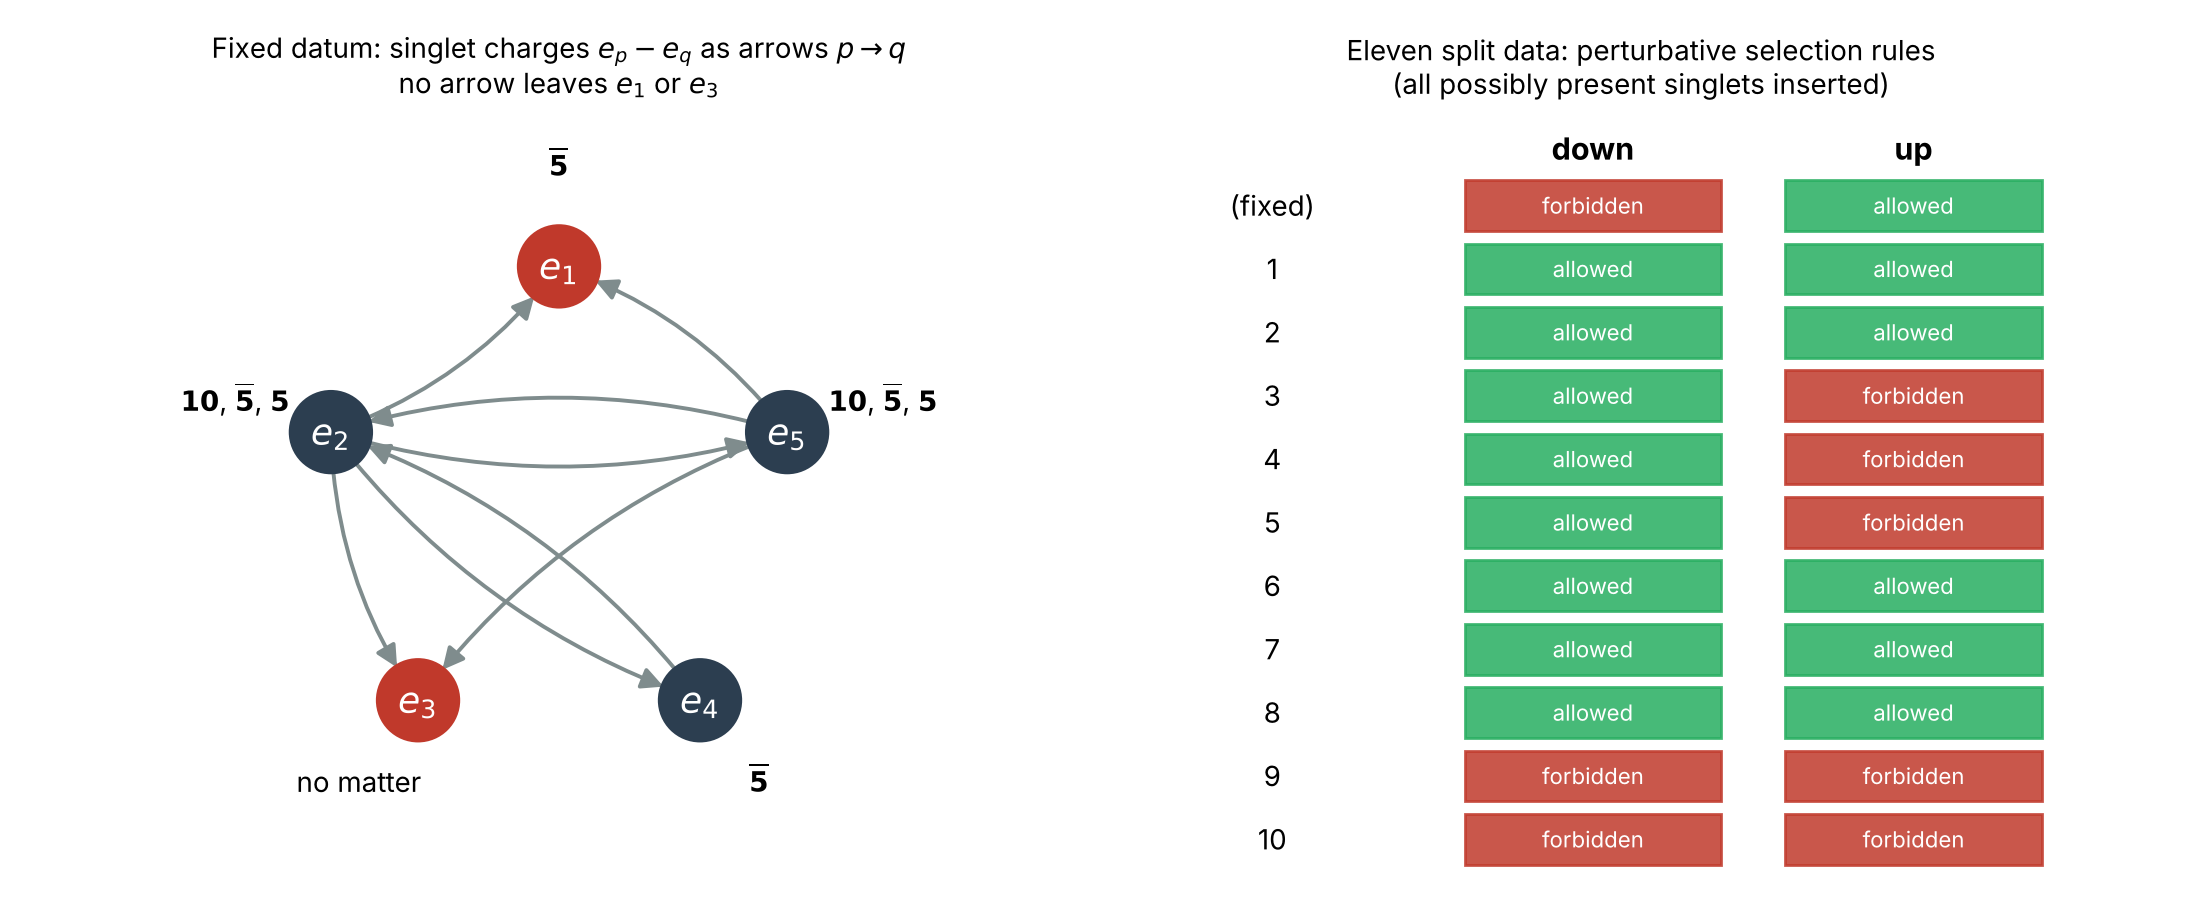
\includegraphics[width=0.96\textwidth]{figures/fig_charges.png}
\caption{Left: the singlet charges $e_p-e_q$ of the fixed datum drawn as
arrows $p\to q$ between the five line bundles, with the charged matter
each bundle carries; no arrow leaves $e_1$ or $e_3$, which is the
certificate of Proposition~\ref{prop:eleven} for the vanishing of $Y_d$.
Right: the outcome of the selection rules for the up-type and down-type
matrices on the eleven split data of Table~\ref{tab:eleven}, with every
possibly present singlet inserted.}
\label{fig:charges}
\end{figure}

\section{Nine-condition ledger for the one fixed datum}\label{sec:ledger}
The table refers only to $X_\pi/\Gamma$, the descended split bundle,
$J=100\sum J_i$, the specified Wilson line and zero singlet expectation
values. The perturbative effective-theory assumptions are stated in
Section~\ref{sec:pointfailure}. ``Verified'' below always carries this
stated mathematical or perturbative scope. Table~\ref{tab:ledger} is
the result.
\begin{table}[t]
\caption{The nine conditions at the fixed datum.}\label{tab:ledger}
\small
\begin{adjustbox}{max width=\linewidth}\begin{tabular}{@{}p{.06\linewidth}>{\raggedright\arraybackslash}p{.18\linewidth}>{\raggedright\arraybackslash}p{.65\linewidth}@{}}
\toprule
&Status&Certificate or failed test\\\midrule
C1&Partial&Polystability, $c_1=0$ and cover anomaly effectivity proved;
integral quotient anomaly and quantized hidden completion not certified.\\
C2&Verified&Descended bundle index is exactly $-3$.\\
C3&Fails at split point&The $SU(5)$ centralizer is the SM subgroup,
but the additional generator $q$ in \eqref{eq:extrau1} survives; forced
for every rank-five split datum by Theorem~\ref{thm:forced}. On the cover
it disappears on the two-block extension branch of
Theorem~\ref{thm:twoblocks}, whose descent to $X_\pi/\Gamma$ and spectrum
are not certified.\\
C4&Verified spectrum&Equivariant cohomology gives three charged families
and no additional chiral charged exotics.\\
C5&Vacant charged-exotic test&No additional massless charged vectorlike
exotics occur in this spectrum. Neutral and hidden masses not asserted.\\
C6&Verified spectrum&One Higgs doublet pair and no massless Higgs triplets
after the fixed Wilson projection.\\
C7&Fails at tree level&The volume ray is flat in the stated classical
F- and D-term potential, so the volume modulus is massless there and
C7$_W$ fails for every $m_0>0$.\\
C8&Fails perturbatively&$\operatorname{rank}Y_u\le2$ and $Y_d=0$ at the
fixed zero-singlet point; normalization cannot repair rank, and no singlet
insertion restores $Y_d$ (Proposition~\ref{prop:eleven}); C8$_W$ fails
for every window.\\
C9&Not certified&No supersymmetry-breaking sector has been constructed;
at the fixed point all F- and D-terms vanish, so the first clause of
C9$_W$ is not met there.\\\bottomrule
\end{tabular}\end{adjustbox}
\end{table}
Thus the fixed datum is \emph{not} a viable nine-condition vacuum.
The construction proves explicit geometry and charged-spectrum statements,
and it proves definite failures of some tests. It neither proves nor
disproves existence of a different vacuum passing all nine.

\section{An estimate for coupling the stabilization sectors}\label{sec:blocks}
Independent stabilization calculations cannot be joined without bounding
their mixed derivatives. The following elementary estimate states one
usable quantitative requirement.
\begin{proposition}[Mixed-sector Hessian bound]\label{prop:blockhessian}
Let the real symmetric Hessian have blocks
$H=\left(\begin{smallmatrix}A&B\\B^T&C\end{smallmatrix}\right)$,
with $A\succeq\alpha I$, $C\succeq\gamma I$ and
$\|B\|_{\rm op}\le\beta$, where $\alpha,\gamma>0$.
If $\beta^2<\alpha\gamma$, then
\[
 H\succeq\frac{\alpha+\gamma-
 \sqrt{(\alpha-\gamma)^2+4\beta^2}}2 I>0.
\]
\end{proposition}
\begin{proof}
For vectors $v,w$, the quadratic form is bounded below by
$\alpha\|v\|^2-2\beta\|v\|\|w\|+\gamma\|w\|^2$.
The least eigenvalue of the two-by-two coefficient matrix is the
displayed expression; its positivity is equivalent to the stated
determinant inequality and positive trace.
\end{proof}
This is a sufficient criterion with inputs to be measured or proved on
a compactification chart. It does not provide those inputs for $X_\pi$.


\section{Why holomorphic masses do not close C8}
After fixing conventions and the Higgs factor, a physical Yukawa matrix
has the form
\begin{equation}\label{eq:normalisation}
 Y_{\rm phys}=c\,Z_L^{-T/2}Y_{\rm hol}Z_R^{-1/2},
 \qquad c>0,
\end{equation}
where the matter metrics are positive definite. Their invertibility
preserves rank but does not preserve singular-value ratios.

\begin{proposition}[A normalization counterexample]\label{prop:normalisation}
For $0<\epsilon<1$, take
\[
Y_{\rm hol}=\operatorname{diag}(\epsilon^8,\epsilon^4,1),\quad
Z_L=I,\quad Z_R=\operatorname{diag}(\epsilon^{16},\epsilon^8,1),\quad c=1.
\]
All metrics are positive definite and $Y_{\rm phys}=I$. Thus a full-rank
holomorphic matrix with separated scales does not prove a physical hierarchy.
\end{proposition}
\begin{proof}
The positive inverse square root of $Z_R$ is
$\operatorname{diag}(\epsilon^{-8},\epsilon^{-4},1)$. Multiplication in
\eqref{eq:normalisation} gives the identity.
\end{proof}
The example does not claim that these metrics occur in the tetraquadric
model. It refutes the inference based on a holomorphic matrix alone.
It does not refute a hierarchy proved with regular nondegenerate metrics
at the limiting point, as the following bound makes precise.

\begin{proposition}[Bounded normalization preserves orders]\label{prop:bounded}
Suppose $mI\preceq Z_L,Z_R\preceq MI$ with $0<m\le M$ and
$0<c_-\le c\le c_+$. For every singular value, ordered consistently,
\[
 \frac{c_-}{M}\sigma_i(Y_{\rm hol})
 \le\sigma_i(Y_{\rm phys})
 \le\frac{c_+}{m}\sigma_i(Y_{\rm hol}).
\]
If these bounds are uniform as a parameter tends to zero, any nonzero
power-law orders of the holomorphic singular values are preserved.
\end{proposition}
\begin{proof}
For invertible $A,B$, the min--max characterization gives
$\sigma_i(AYB)\le\|A\|_{\rm op}\|B\|_{\rm op}\sigma_i(Y)$.
Apply this also to $Y=A^{-1}(AYB)B^{-1}$ to obtain the reverse bound.
The operator norms of the inverse square roots are at most $m^{-1/2}$
and those of their inverses at most $M^{1/2}$; transpose has the same
singular values. Multiplication by $c$ yields the result. Uniform positive
constants do not change a power-law order.
\end{proof}
Continuity and positive definiteness at a regular limiting point give
such bounds locally. The preceding counterexample loses that lower bound
as $\epsilon\to0$. Conversely, an asymptotic order calculation alone does
not fix the observed mass ratios or the point selected by stabilization.
Published physical-flavour constructions are available \cite{CLLN};
that paper leaves stabilization and supersymmetry breaking untreated.
This is a limitation of the result cited, not an assertion about every
heterotic model in the literature.

\section{A quantitative simultaneous-persistence criterion}
The following theorem identifies bounds that would make a local
construction robust. All its assumptions must be checked on the same
compactification chart and in the same normalization.

\begin{theorem}[A certified interior minimum]\label{thm:minimum}
Let $B=\overline B_r(u_0)\subset\mathbb R^n$ and let $V_0,\Delta$
be $C^2$ on a neighborhood of $B$. Suppose on $B$ that
\[
 D^2V_0\succeq\lambda I,\quad
 \|D^2\Delta\|_{\rm op}\le b<\lambda,\quad
 \|\nabla V_0(u_0)\|\le\eta,\quad
 \|\nabla\Delta(u_0)\|\le a.
\]
Put $\kappa=\lambda-b$ and assume $\eta+a<\kappa r$.
Then $V=V_0+\Delta$ has exactly one critical point $u_*$ in $B$.
It is an interior minimum, $D^2V(u_*)\succeq\kappa I$, and
\begin{equation}\label{eq:displacement}
 \|u_*-u_0\|\le\delta:=\frac{\eta+a}{\kappa}<r.
\end{equation}
\end{theorem}
\begin{proof}
The Hessian of $V$ is bounded below by $\kappa I$. Integrating along
a segment yields strong monotonicity:
\[
 (\nabla V(x)-\nabla V(y))\cdot(x-y)\ge\kappa\|x-y\|^2.
\]
For $x$ on the boundary and $v=x-u_0$ this gives
$\nabla V(x)\cdot v\ge\kappa r^2-(\eta+a)r>0$.
The inward directional derivative is negative, so a minimum on the
compact ball cannot occur at its boundary. A minimum exists and is
therefore critical in the interior. Strong monotonicity excludes two
critical points. Apply it with $x=u_*$, $y=u_0$ and use
$\nabla V(u_*)=0$ to obtain
$\kappa\|u_*-u_0\|^2\le(\eta+a)\|u_*-u_0\|$,
which proves \eqref{eq:displacement}.
\end{proof}

\begin{proposition}[Preserving masses and inequalities]\label{prop:persistence}
In Theorem~\ref{thm:minimum}, suppose $Y$ is a physical $3\times3$ Yukawa
matrix with $\|Y(u)-Y(u_0)\|_{\rm op}\le L\|u-u_0\|$ on $B$.
If $s_i$ are its singular values at $u_0$, then at $u_*$ they differ
from $s_i$ by at most $e=L\delta$. In particular $s_{\min}>e$
certifies full rank. For $s_j>e$,
\[
 \frac{\max(0,s_i-e)}{s_j+e}
 \le\frac{s_i(u_*)}{s_j(u_*)}
 \le\frac{s_i+e}{s_j-e}.
\]
If a real acceptance function $q$ is $L_q$-Lipschitz and has required
lower bound $q_{\rm req}$, then
$q(u_0)>q_{\rm req}+L_q\delta$ certifies $q(u_*)>q_{\rm req}$.
\end{proposition}
\begin{proof}
The min--max formula for singular values and
$|\|Av\|-\|Bv\||\le\|(A-B)v\|$ on unit vectors give
$|\sigma_i(A)-\sigma_i(B)|\le\|A-B\|_{\rm op}$ by applying the
formula in both directions. The ratio bounds follow by bounding numerator
and denominator separately. The last assertion is the Lipschitz inequality.
\end{proof}

Thus a controlled ball preserving the discrete spectrum and satisfying
strict mass, hierarchy and consistency margins would turn an approximate
minimum into a simultaneous certificate. If the real kinetic matrix obeys
$0<G(u_*)\preceq\Lambda I$, the physical scalar mass matrix
$G(u_*)^{-1/2}D^2V(u_*)G(u_*)^{-1/2}$ has eigenvalues at least
$\kappa/\Lambda$. This follows by applying the Hessian lower bound to
$G^{-1/2}v$. At a critical point the connection correction to the Hessian
vanishes. Thus kinetic normalization must also be bounded when interpreting
the Hessian physically. The bounds must include all
claimed perturbative and nonperturbative corrections, the normalization
metrics, the physical moduli coordinates, and any constraints or gauge
quotients. A Hessian estimate for a freely invented scalar function is
not a Hessian estimate for the compactification potential.

\section{An explicit local effective-theory construction and its limit}
It is useful to separate a solvable analytic problem from the missing
string realization. Consider a classical global $N=1$ effective theory
with fields $S,Z_1,\ldots,Z_m$, constants $a>0$, $F\ne0$, and $m_j\ne0$:
\[
 K=|S|^2-a|S|^4+\sum_j|Z_j|^2,
 \qquad W=FS+\frac12\sum_jm_jZ_j^2.
\]
We work on $|S|^2<1/(4a)$, where its K\"ahler metric is positive.

\begin{proposition}[A stabilized local model]\label{prop:eft}
For this specified classical global effective theory,
\[
 V=\frac{|F|^2}{1-4a|S|^2}+\sum_j|m_j|^2|Z_j|^2
\]
has a unique minimum at the origin of the stated domain. Supersymmetry
is broken there. In canonical real coordinates its Hessian has diagonal
entries $4a|F|^2,4a|F|^2$ and $|m_j|^2,|m_j|^2$ for each $j$.
\end{proposition}
\begin{proof}
$K_{S\bar S}=1-4a|S|^2$ and $K_{Z_i\bar Z_j}=\delta_{ij}$, so the
global-supersymmetry potential $K^{A\bar B}W_A\overline W_B$ is the
displayed expression. Its first term is strictly increasing with $|S|^2$
and the remaining terms are positive quadratics. The auxiliary field in
the $S$ direction is nonzero at zero because $W_S=F$. Expanding with
$S=(x+iy)/\sqrt2$ gives
$V=|F|^2+2a|F|^2(x^2+y^2)+\sum_j|m_j|^2(u_j^2+v_j^2)/2+O(|S|^4)$,
which proves the Hessian assertion.
\end{proof}
This proposition supplies no Calabi--Yau bundle realizing its $K$ and $W$.
It omits supergravity, flux quantization, the anomaly constraints and
the coupled visible sector. Consequently it verifies neither C7 nor C9
for the geometric example. Its role is to make the missing realization
problem explicit rather than hide it inside a choice of coefficients.

\begin{proposition}[A tree-level obstruction]\label{prop:noscale}
Let a supergravity model have
\[
 K=K_0(z,\bar z)-\sum_{i=1}^r n_i\log(T_i+\bar T_i),
 \quad n_i>0,\quad\sum_i n_i=3,\quad W=W(z).
\]
At a point with $D_zW=0$, its F-term potential vanishes for all $T_i$
in this product chart. It does not stabilize these K\"ahler directions.
\end{proposition}
\begin{proof}
The $T$-block is diagonal,
$K_i=-n_i/(T_i+\bar T_i)$ and
$K_{i\bar i}=n_i/(T_i+\bar T_i)^2$. Hence
$\sum_iK^{i\bar i}K_iK_{\bar i}=\sum_i n_i=3$.
Since $D_iW=K_iW$ and the $z$ block contributes zero, these terms cancel
the $-3|W|^2$ in $V_F=e^K(K^{A\bar B}D_AW\overline{D_BW}-3|W|^2)$.
Thus there are flat $T$ directions. Additional D terms or corrections are
not covered by this assertion and would need their own calculation.
\end{proof}




\section{Conclusion and verification scope}\label{sec:conclusion}
The algebraic spectral calculation and the existence of a viable vacuum
are separate statements. The mirror argument restricts a selector on its
specified domain; it does not supply a point outside that domain.
The explicit tetraquadric construction supplies a free quotient, index
and projected charged spectrum at one fixed complex structure.
Its residual gauge generator and deficient perturbative Yukawa matrices
are exact obstructions to using that split point as the sought vacuum.
The extension branch changes the bundle and therefore requires its own
stability, operator and potential calculations before replacing the audit.
Section~\ref{sec:splitbranch} shows that this branch is the only one left
on the tetraquadric: no sum of five line bundles on a threefold with at
most four K\"ahler parameters passes the gauge condition at its split
locus, and on the tetraquadric the selection rules already remove six of
the eleven three-family split data from the Yukawa condition. On the
branch itself a single extension never removes the forced gauge boson,
while two rank-two extensions do so for the fixed datum and for five of
the ten further data, on the cover and on one side of a stability wall,
and cannot do so for the other four. What the branch has not been shown
to do is to descend to the quotient, to keep three families with the
required Yukawa matrices, and to lift the flat directions of
C7$_W$; the four classes closed at the two smallest shapes could only
pass C3 on a shape with a block of rank three or more. With the windows of
Definition~\ref{def:windows} the conjecture is a definite statement, and
every failure recorded here is independent of them.

The remaining task is to specify a single quantized compactification
with its hidden sector and controlled effective potential, and to verify
all nine predicates at its stabilized point. The estimates in this paper
state sufficient analytic conditions for parts of that task. Their
inputs have not been established for the fixed example. Consequently this
manuscript does not prove the full Geometric Selection Conjecture.

\section*{Data and declarations}
The spectral sections and their five appendices present the work of the
two authors on the Dwork and weighted Fermat pencils \cite{Dwork}; the
mirror argument is that of \cite{Mirror} under its standard-type
partial-mirror convention; the marked-point and effective-theory criteria
reorganize \cite{Paper10}. The bundle example is the published one of
\cite{BCL}, and the ten further line-bundle sums of
Section~\ref{sec:eleven} were produced by the scan of \cite{Anaxia}.

Python programs recompute the smooth-seed polynomial identities, the
fixed-pencil determinant and character cohomology, the Dwork label,
coupling and mass-map counts, the thirteen-row Chern and index arithmetic,
the selection rules of Proposition~\ref{prop:eleven} with their flow
certificates, and the slope spaces, orientations, extension dimensions and
polystable points of Theorem~\ref{thm:twoblocks} with the permutation
matrices of Lemma~\ref{lem:genericvanishing}. Each program emits a machine-readable result with its scope.
They are in the repository
\href{https://github.com/creelie/geometric-selection-conjecture}{\texttt{creelie/geometric-selection-conjecture}} on GitHub (release
\ownrelease{}, concept DOI \href{https://doi.org/\ownconceptdoi}{\ownconceptdoi}).
Finite algebra checks do not certify string corrections, stabilize moduli,
or supply a proof of all nine conditions; no statement of the paper rests
on them alone.

\smallskip\noindent\textit{Funding.} This research received no external
funding.

\smallskip\noindent\textit{Conflicts of interest.} The authors declare no
conflict of interest.

\appendix


\section{The Hessian in the socle}\label{app:hessian}

The Hessian matrix of $F_\psi$ has entries
\[
H_{ii}=20\,x_i^3,\qquad H_{ij}=-5\psi\prod_{k\ne i,j}x_k\quad(i\ne j).
\]
For a permutation $\pi$ of $\{1,\dots,5\}$ with $m$ moved points and
$f=5-m$ fixed points, the product $\prod_iH_{i\pi(i)}$ is
$20^f(-5\psi)^m$ times a monomial whose exponents are read off as follows.
A fixed coordinate $a$ receives $3$ from its diagonal entry and $1$ from each
of the $m$ off-diagonal entries, since an off-diagonal entry $(i,\pi(i))$
omits only the moved coordinates $i$ and $\pi(i)$. A moved coordinate $c$
is omitted by exactly two off-diagonal entries, those with $i=c$ and with
$\pi(i)=c$, which are different because $\pi(c)\ne c$; it receives $1$ from
each of the other $m-2$. Hence the monomial of $\pi$ is
\[
\prod_{a\ \mathrm{fixed}}x_a^{3+m}\prod_{c\ \mathrm{moved}}x_c^{m-2},
\]
of degree $f(3+m)+m(m-2)=15$, and it depends only on the number of moved
points. The five values of $m$ give:
\begin{itemize}[leftmargin=*,itemsep=1pt]
\item $m=0$: the monomial $m_0=(3,3,3,3,3)$, sector $0$;
\item $m=2$: $(5,5,5,0,0)$ up to order, sector $3$, so $\lambda=\psi^3$;
\item $m=3$: $(6,6,1,1,1)$ up to order, sector $2$, so $\lambda=\psi^2$;
\item $m=4$: $(7,2,2,2,2)$ up to order, sector $1$, so $\lambda=\psi$;
\item $m=5$: $(3,3,3,3,3)$, sector $0$.
\end{itemize}
The contribution of a permutation to $H(\psi)=\lambda(\Hess F_\psi)$ is
$\operatorname{sgn}(\pi)\,20^f(-5\psi)^m\psi^{r(m)}$ with $r(0)=r(5)=0$,
$r(2)=3$, $r(3)=2$, $r(4)=1$, so $m+r(m)=5$ for every $m\ge2$ and every
non-identity permutation contributes a multiple of $\psi^5$. The cycle
types are
\[
\begin{aligned}
&1^5:\ 1\ \text{permutation, }m=0,\ +20^5=3\,200\,000;\\
&2\,1^3:\ 10,\ \text{odd},\ m=2:\ 10\cdot(-1)\cdot20^3\cdot25=-2\,000\,000;\\
&3\,1^2:\ 20,\ \text{even},\ m=3:\ 20\cdot20^2\cdot(-125)=-1\,000\,000;\\
&4\,1:\ 30,\ \text{odd},\ m=4:\ 30\cdot(-1)\cdot20\cdot625=-375\,000;\\
&2^2\,1:\ 15,\ \text{even},\ m=4:\ 15\cdot20\cdot625=187\,500;\\
&5:\ 24,\ \text{even},\ m=5:\ 24\cdot(-3125)=-75\,000;\\
&3\,2:\ 20,\ \text{odd},\ m=5:\ 20\cdot(-1)\cdot(-3125)=62\,500,
\end{aligned}
\]
where the last six numbers are the coefficients of $\psi^5$. The counts
$1+10+20+30+15+24+20$ add up to $120$. The coefficients of $\psi^5$ add up
to $-3\,200\,000$, which gives $H(\psi)=3\,200\,000(1-\psi^5)$.

\section{The coupling count}\label{app:count}

\subsection{Ordered triples by sector}

For $\ee$ of degree fifteen, $O(\ee)$ is the number of ordered triples
$(\va,\bb,\cc)\in B^3$ with $\va+\bb+\cc=\ee$. We count it by the third
label: for each $\cc\in B$ with $\cc\le\ee$, put $\mathbf s=\ee-\cc$, a
vector of degree ten, and count the $\va\in B$ with $\mathbf s-\va\in B$,
that is, with
\[
\max(0,s_i-3)\le a_i\le\min(3,s_i)\quad\text{for all }i,\qquad
\textstyle\sum a_i=5.
\]
This number $N(\mathbf s)$ is the coefficient of $t^5$ in
$\prod_i\big(t^{\max(0,s_i-3)}+\dots+t^{\min(3,s_i)}\big)$. Write
$[n]=1+t+\dots+t^{n-1}$.

\emph{Sector $0$, $\ee=(3,3,3,3,3)$.} Here $\mathbf s=3\one-\cc$ has
entries in $\{0,\dots,3\}$, so $N(\mathbf s)$ is the coefficient of $t^5$ in
$\prod_i[s_i+1]$. The multiset of entries of $\mathbf s$ is the complement
of the type of $\cc$:
\[
\begin{array}{l|l|r|r}
\text{type of }\cc&\text{entries of }\mathbf s&\#\cc&N(\mathbf s)\\\hline
\{3,2,0,0,0\}&\{3,3,3,1,0\}&20&24\\
\{3,1,1,0,0\}&\{3,3,2,2,0\}&30&28\\
\{2,2,1,0,0\}&\{3,3,2,1,1\}&30&38\\
\{2,1,1,1,0\}&\{3,2,2,2,1\}&20&44\\
\{1,1,1,1,1\}&\{2,2,2,2,2\}&1&51
\end{array}
\]
The values of $N$ are central coefficients. For $\{3,3,3,1,0\}$,
$[4]^3=1+3t+6t^2+10t^3+12t^4+12t^5+\cdots$ and the factor $[2]$ gives
$12+12=24$. For $\{3,3,2,2,0\}$, $[4]^2=(1,2,3,4,3,2,1)$ and
$[3]^2=(1,2,3,2,1)$, so the coefficient is $2+6+12+6+2=28$. For
$\{3,3,2,1,1\}$, $[3][2]^2=(1,3,4,3,1)$ and the coefficient is
$2+9+16+9+2=38$. For $\{3,2,2,2,1\}$, $[3]^3=(1,3,6,7,6,3,1)$ and
$[4][2]=(1,2,2,2,1)$, so the coefficient is $3+12+14+12+3=44$. For
$\{2,2,2,2,2\}$ the coefficient of $t^5$ in $(1+t+t^2)^5$ is $51$. Hence
\[
O(3,3,3,3,3)=20\cdot24+30\cdot28+30\cdot38+20\cdot44+51=3391.
\]
(The table for $\ee=(3,3,3,3,3)$ also shows that every $\cc\in B$ occurs,
since $\mathbf s=3\one-\cc$ always admits some $\va$.)

\emph{Sector $1$, $\ee=(7,2,2,2,2)$.} Since $a_1+b_1\le6$, $c_1\ge1$, and
$c_i\le2$ for $i\ge2$. With $\mathbf s=\ee-\cc$, the entry $s_1=7-c_1$
forces $a_1\ge4-c_1$, and the remaining entries $s_i=2-c_i\le2$ impose only
$a_i\le s_i$. Grouping $\cc$ by $c_1$ and by the multiset of
$(c_2,\dots,c_5)$:
\[
\begin{array}{l|l|r|r|r}
c_1&(c_2,\dots,c_5)&\#\cc&N(\mathbf s)&\text{total}\\\hline
1&\{1,1,1,1\}&1&6&6\\
1&\{2,1,1,0\}&12&4&48\\
1&\{2,2,0,0\}&6&3&18\\
2&\{1,1,1,0\}&4&14&56\\
2&\{2,1,0,0\}&12&10&120\\
3&\{1,1,0,0\}&6&26&156\\
3&\{2,0,0,0\}&4&19&76
\end{array}
\]
For instance, when $c_1=3$ and $(c_2,\dots,c_5)=(2,0,0,0)$, $a_1$ ranges
over $\{1,2,3\}$ and the other entries satisfy $a_i\le(0,2,2,2)$ with sum
$5-a_1$; the coefficients of $t^4$, $t^3$, $t^2$ in $[3]^3$ are $6$, $7$,
$6$, which add to $19$. The total is $O(7,2,2,2,2)=480$.

\emph{Sector $2$, $\ee=(6,6,1,1,1)$.} Here $c_3,c_4,c_5\le1$, and the same
grouping gives
\[
\begin{array}{l|l|r|r|r}
\{c_1,c_2\}&(c_3,c_4,c_5)&\#\cc&N(\mathbf s)&\text{total}\\\hline
\{1,1\}&\{1,1,1\}&1&2&2\\
\{2,0\}&\{1,1,1\}&2&1&2\\
\{2,1\}&\{1,1,0\}&6&4&24\\
\{2,2\}&\{1,0,0\}&3&10&30\\
\{3,0\}&\{1,1,0\}&6&2&12\\
\{3,1\}&\{1,0,0\}&6&8&48\\
\{3,2\}&\{0,0,0\}&2&22&44
\end{array}
\]
and $O(6,6,1,1,1)=162$.

\emph{Sector $3$, $\ee=(5,5,5,0,0)$.} Here $c_4=c_5=0$ and
$c_1+c_2+c_3=5$. For $\{c_1,c_2,c_3\}=\{2,2,1\}$ the entries of
$\mathbf s$ are $(3,3,4)$, the bounds are $a_i\le3$ on the first two and
$1\le a_3\le3$, and the coefficient of $t^5$ in $[4]^2(t+t^2+t^3)$ is
$3+4+3=10$; for $\{3,1,1\}$ the entries are $(2,4,4)$ and the coefficient of
$t^5$ in $[3](t+t^2+t^3)^2$ is $2+3+2=7$; for $\{3,2,0\}$ the entries are
$(2,3,5)$ and the coefficient of $t^5$ in $[3][4](t^2+t^3)$ is $3+3=6$. With
three, three and six choices of $\cc$, $O(5,5,5,0,0)=30+21+36=87$.

The ordered counts by sector are $O_0=3391$, $O_1=5\cdot480=2400$,
$O_2=10\cdot162=1620$ and $O_3=10\cdot87=870$, with total $8281$ in
agreement with Section~\ref{sec:count}.

\subsection{Repeated labels}

For $\va\in B$ the partner $\cc$ with $2\va+\cc$ in a sector is found type
by type, as in the proof of Theorem~\ref{thm:C}. For $\va=\one$, $\cc=\one$
in sector $0$. For $\va$ of type $\{2,1,1,1,0\}$, sector $1$ gives
$c_i\equiv2-2a_i$, that is $\cc$ with a three where $\va$ has its two, a two
where $\va$ has its zero and zeros elsewhere, of sum five. For type
$\{3,1,1,0,0\}$, sector $1$ gives a one where $\va$ has its three, zeros
where it has ones and twos where it has zeros. For type $\{3,2,0,0,0\}$,
sector $2$ gives zero, two and ones. For type $\{2,2,1,0,0\}$, sector $3$
gives ones at the twos, a three at the one and zeros elsewhere. In each case
the other sectors produce a residue four or a total different from five.
So the hundred triples $\{\va,\va,\cc\}$ with $\cc\ne\va$ lie $20+30=50$ in
sector $1$, $20$ in sector $2$ and $30$ in sector $3$, and none in sector
$0$, which is the list $D_r=0,50,20,30$ used in Section~\ref{sec:count}.

\section{Hodge norms at the Fermat point}\label{app:fermat}

This appendix proves Proposition~\ref{prop:fermat}. Write
$G=\mu_5^5/\mu_5$ for the group of diagonal phases of $\PP^4$, which acts
on $X_0$. For $\mathbf k\in\{1,2,3,4\}^5$ with $\sum k_i\equiv0\pmod5$ let
$\chi_{\mathbf k}(a)=\zeta^{a\cdot\mathbf k}$.

\subsection{Eigenlines}

The character $\chi_{\mathbf k}$ occurs in $H^3(X_0,\C)$ exactly once, and
these are all the characters that occur: the number of such $\mathbf k$ is
$\frac15\sum_{j=0}^4\big(\sum_{k=1}^4\zeta^{jk}\big)^5=\frac15(4^5-4)=204
=b_3(X_0)$, and each occurs at least once because the residue
$\Res(x^{\mathbf k-\one}\Omega_0/F^{q+1})$, $5(q+1)=\sum k_i$, is a nonzero
class of character $\chi_{\mathbf k}$ (Griffiths' theorem and the fact that
$x^{\mathbf k-\one}$, with exponents at most three, is nonzero in the
Jacobian ring $\C[x]/(x_1^4,\dots,x_5^4)$ of the Fermat quintic). In
particular $\omega_{\bb}$ spans the line of $\mathbf k=\bb+\one$.

\subsection{The bilinear relation}

Let $Q$ be the intersection form on $H_3(X_0,\Z)$, extended to complex
coefficients, and identify $H^3$ with $H_3$ by Poincar\'e duality $D$, so
that $\int_c\omega=Q(c,D\omega)$ and $\int_{X_0}\omega\wedge\eta=
Q(D\omega,D\eta)$. Since $Q$ is $G$-invariant, it pairs the eigenline $L$ of
$\chi$ only with the eigenline $L'$ of $\bar\chi$. Let $e$ be an integral
cycle and $u$ its component in $L'$; its component in $L$ is $\bar u$,
because $e$ is real. If $D\omega_{\bb}=\alpha\bar u$ with $\bar u\ne0$, then
\[
\int_e\omega_{\bb}=Q(e,\alpha\bar u)=\alpha\,Q(u,\bar u),\qquad
\int_{X_0}\omega_{\bb}\wedge\overline{\omega_{\bb}}=|\alpha|^2Q(\bar u,u),
\]
and therefore
\begin{equation}\label{eq:bilinear}
g_{\bb}=\Big|\int_{X_0}\omega_{\bb}\wedge\overline{\omega_{\bb}}\Big|
=\frac{|\int_e\omega_{\bb}|^2}{|Q(u,\bar u)|}.
\end{equation}
It remains to compute both sides for one cycle.

\subsection{The cycle of Pham}

On the affine chart $x_5=1$ put $y_i=x_i/x_5$; the open part of $X_0$ is
$U=\{f=0\}$, $f=y_1^5+y_2^5+y_3^5+y_4^5+1$, and $\mu_5^4$ acts by
$y_i\mapsto\zeta^{a_i}y_i$. A character $\mathbf k$ of $G$ restricts to the
character $(k_1,k_2,k_3,k_4)$ of $\mu_5^4$, and $k_5\equiv-(k_1+k_2+k_3+
k_4)$. Pham~\cite{Pha65} showed that $U$ retracts onto the join of four
copies of the set of fifth roots of $-1$, and that $H_3(U,\Z)$ is generated
over $\Z[\mu_5^4]$ by the cycle
\[
e=(1-T_1)(1-T_2)(1-T_3)(1-T_4)\,\Delta,
\]
where $\Delta$ is the real simplex $\{y_i=\epsilon v_i,\ v_i\ge0,\
\sum v_i^5=1\}$ with $\epsilon^5=-1$, and $T_i$ multiplies $y_i$ by
$\zeta$.

\emph{The period.} By Griffiths' residue formula,
$\int_e\omega_{\bb}=\frac1{2\pi i}\int_{\tau(e)}x^{\bb}\Omega_0/F^2$ with
$\tau$ the tube map. On the chart this is the integral of
$y^{\bb'}dy/f^2$, $\bb'=(b_1,\dots,b_4)$. Put $f_s=\sum y_i^5+s$; then
$y^{\bb'}dy/f_s^2=-\partial_s(y^{\bb'}dy/f_s)$, and
$\frac1{2\pi i}\int_{\tau(e)}y^{\bb'}dy/f_s=\int_{e_s}y^{\bb'}dy/df_s$
with the Gelfand--Leray form. The substitution $y=s^{1/5}u$ shows that the
last integral is $s^{A}P$ with $A=\frac15\sum_{i\le4}k_i-1$ and $P$ its value
at $s=1$. Differentiating at $s=1$,
\[
\int_e\omega_{\bb}=-A\,P.
\]
On $\Delta$, with $t_i=v_i^5$, the Gelfand--Leray form is
$5^{-4}\prod_it_i^{1/5-1}dt$ on the simplex $\sum t_i=1$, and
$y^{\bb'}=\epsilon^{|\bb'|}\prod t_i^{b_i/5}$; Dirichlet's integral gives
$\int_\Delta=\epsilon^{|\bb'|+4}5^{-4}\prod_{i\le4}\Gamma(k_i/5)/
\Gamma(\sum_{i\le4}k_i/5)$, and each factor $1-T_i$ multiplies it by
$1-\zeta^{k_i}$. Since $\sum_{i\le4}k_i=10-k_5$, $A=1-k_5/5$ and
$\Gamma(A+1)=A\,\Gamma(A)$, so
\begin{equation}\label{eq:period}
\Big|\int_e\omega_{\bb}\Big|=5^{-4}\prod_{i=1}^4\big|1-\zeta^{k_i}\big|
\,\frac{\prod_{i=1}^4\Gamma(k_i/5)}{\Gamma(1-k_5/5)}.
\end{equation}

\emph{The intersection number.} For one variable, the reduced homology of
the fibre $\{y^5=-1\}$ is the augmentation ideal $I$ of $\Z[t]/(t^5-1)$,
the monodromy is multiplication by $t$, and the variation operator is
multiplication by $t-1$. The Seifert form $L(x,z)=\ip{x}{\mathrm{Var}^{-1}z}$
is therefore, in terms of the values $\hat x(k)=x(\zeta^k)$,
\[
L(x,z)=\frac15\sum_{k=1}^4\frac{\hat x(k)\,\hat z(-k)}{\zeta^{-k}-1}.
\]
By the theorem of Sebastiani and Thom~\cite{ST71}, in the form of
Sakamoto~\cite{Sak74} for Seifert forms, the Seifert form of
$y_1^5+\dots+y_4^5$ is, up to sign, the tensor product of four copies, and
the intersection form on the three-dimensional fibre is $Q=-L+L^{T}$. On the
eigenline of $(k_1,\dots,k_4)$ this gives
\[
Q(x,z)=\pm\frac1{5^4}\,\hat x(\mathbf k)\hat z(-\mathbf k)\Big(
\prod_{i\le4}\frac1{\zeta^{k_i}-1}-\prod_{i\le4}\frac1{\zeta^{-k_i}-1}\Big).
\]
With four factors, $\prod(\zeta^{k_i}-1)=\zeta^{\sum k_i}\prod(\zeta^{-k_i}
-1)$, so the bracket has absolute value
\[
\frac{|1-\zeta^{k_1+k_2+k_3+k_4}|}{\prod_{i\le4}|1-\zeta^{k_i}|^2}
=\frac{|1-\zeta^{k_5}|}{\prod_{i\le4}|1-\zeta^{k_i}|^2}.
\] The cycle $e$ has
$\hat e(\mathbf k)=\prod_{i\le4}(1-\zeta^{k_i})$ up to a unimodular factor,
so its component $u$ satisfies
\begin{equation}\label{eq:intersection}
|Q(u,\bar u)|=5^{-4}\prod_{i=1}^5\big|1-\zeta^{k_i}\big|.
\end{equation}
This is nonzero, so $\bar u\ne0$, as needed in \eqref{eq:bilinear}.

\subsection{Conclusion of the proof}

Inserting \eqref{eq:period} and \eqref{eq:intersection} in
\eqref{eq:bilinear},
\[
g_{\bb}=5^{-4}\,\prod_{i=1}^4\big|1-\zeta^{k_i}\big|\Gamma(k_i/5)^2\cdot
\frac{1}{|1-\zeta^{k_5}|\,\Gamma(1-k_5/5)^2}.
\]
With $|1-\zeta^k|=2\sin(\pi k/5)$ and $\Gamma(t)\Gamma(1-t)=\pi/\sin\pi t$,
\[
2\sin(\pi t)\,\Gamma(t)^2=2\pi\,\gamma(t),\qquad
\frac{1}{2\sin(\pi t)\,\Gamma(1-t)^2}=\frac{\gamma(t)}{2\pi},
\]
so $g_{\bb}=5^{-4}(2\pi)^3\prod_{i=1}^5\gamma(k_i/5)$, which is
\eqref{eq:gamma} with $C=(2\pi)^3/5^4$. The class of $\Omega$, with
$\mathbf k=\one$, has no derivative in the period computation, so
$|\int_e\Omega|=|P|$ with $\Gamma(\sum_{i\le4}k_i/5)=\Gamma(4/5)=
\Gamma(1-k_5/5)$, and the same formula holds: $\|\Omega\|^2=C\gamma(1/5)^5$.
Since $\partial_\psi\Res(\Omega_0/F_\psi)=\Res(5x_1\cdots x_5\Omega_0/
F_\psi^2)=5\omega_{\one}$ and $\omega_{\one}$ is of type $(2,1)$ at
$\psi=0$ (its character differs from that of $\Omega$), the
Weil--Petersson metric at the Fermat point is
\begin{align*}
G_{\psi\bar\psi}(0)&=\frac{25\,g_{\one}}{\|\Omega\|^2}
=25\,\frac{\gamma(2/5)^5}{\gamma(1/5)^5}\\
&=25\,\frac{\Gamma(2/5)^5\Gamma(4/5)^5}{\Gamma(1/5)^5\Gamma(3/5)^5}=0.19226.
\end{align*}

\subsection{Numerical values}

With $\Gamma(1/5)=4.59084$, $\Gamma(2/5)=2.21816$, $\Gamma(3/5)=1.48919$
and $\Gamma(4/5)=1.16423$, $\gamma(1/5)=3.94325$ and $\gamma(2/5)=1.48951$;
$\gamma(3/5)$ and $\gamma(4/5)$ are their inverses. The norms of the
five types follow by multiplying the five factors, and the masses of
Table~\ref{tab:fermat} are their inverses.

\section{Shared characters on the octic and the dectic}\label{app:wlabels}

\begin{table}[t]
\caption{The entries of the blocks of Table~\ref{tab:wblocks}, for the
representative with $(i,j,k,l)=(1,2,3,4)$. Exponent vectors are written in
full; the column $r$ is the sector of $h+\bb+\cc$ and $k$ is the vector of
\eqref{eq:wsector}.}
\label{tab:wblockdata}
\centering
\footnotesize
\begin{adjustbox}{max width=\linewidth}\begin{tabular}{lrlllrll}
\toprule
pencil & row & $\bb$ & $\cc$ & $h+\bb+\cc$ & $r$ & $k$ & entry\\
\midrule
sextic & 1 & $(4,0,0,0,1)$ & $(3,1,1,1,0)$ & $(8,2,2,2,2)$ & $2$ & $(1,0,0,0,1)$ & $2\psi^{2}$\\
 & 1 & $(0,2,2,2,0)$ & $(3,1,1,1,0)$ & $(4,4,4,4,1)$ & $0$ & $(0,0,0,0,0)$ & $1$\\
 & 2 & $(3,3,0,0,0)$ & $(3,3,0,0,0)$ & $(7,7,1,1,1)$ & $3$ & $(1,1,0,0,1)$ & $2\psi^{3}$\\
 & 2 & $(3,3,0,0,0)$ & $(0,0,3,3,0)$ & $(4,4,4,4,1)$ & $0$ & $(0,0,0,0,0)$ & $1$\\
 & 2 & $(0,0,3,3,0)$ & $(3,3,0,0,0)$ & $(4,4,4,4,1)$ & $0$ & $(0,0,0,0,0)$ & $1$\\
 & 2 & $(0,0,3,3,0)$ & $(0,0,3,3,0)$ & $(1,1,7,7,1)$ & $3$ & $(0,0,1,1,1)$ & $2\psi^{3}$\\
\midrule
octic & 1 & $(6,1,1,0,0)$ & $(4,1,1,2,0)$ & $(12,4,4,4,0)$ & $2$ & $(1,0,0,0,1)$ & $4\psi^{2}$\\
 & 1 & $(0,3,3,2,0)$ & $(4,1,1,2,0)$ & $(6,6,6,6,0)$ & $0$ & $(0,0,0,0,0)$ & $1$\\
 & 2 & $(6,2,0,0,0)$ & $(2,6,0,0,0)$ & $(10,10,2,2,0)$ & $4$ & $(1,1,0,0,2)$ & $16\psi^{4}$\\
 & 2 & $(6,2,0,0,0)$ & $(4,0,2,2,0)$ & $(12,4,4,4,0)$ & $2$ & $(1,0,0,0,1)$ & $4\psi^{2}$\\
 & 2 & $(0,4,2,2,0)$ & $(2,6,0,0,0)$ & $(4,12,4,4,0)$ & $2$ & $(0,1,0,0,1)$ & $4\psi^{2}$\\
 & 2 & $(0,4,2,2,0)$ & $(4,0,2,2,0)$ & $(6,6,6,6,0)$ & $0$ & $(0,0,0,0,0)$ & $1$\\
 & 3 & $(4,4,0,0,0)$ & $(4,4,0,0,0)$ & $(10,10,2,2,0)$ & $4$ & $(1,1,0,0,2)$ & $16\psi^{4}$\\
 & 3 & $(4,4,0,0,0)$ & $(0,0,4,4,0)$ & $(6,6,6,6,0)$ & $0$ & $(0,0,0,0,0)$ & $1$\\
 & 3 & $(0,0,4,4,0)$ & $(4,4,0,0,0)$ & $(6,6,6,6,0)$ & $0$ & $(0,0,0,0,0)$ & $1$\\
 & 3 & $(0,0,4,4,0)$ & $(0,0,4,4,0)$ & $(2,2,10,10,0)$ & $4$ & $(0,0,1,1,2)$ & $16\psi^{4}$\\
\midrule
dectic & 1 & $(2,1,1,3,0)$ & $(2,3,3,1,0)$ & $(6,6,6,6,0)$ & $2$ & $(0,0,0,1,1)$ & $10\psi^{2}$\\
 & 1 & $(4,3,3,0,0)$ & $(2,3,3,1,0)$ & $(8,8,8,3,0)$ & $0$ & $(0,0,0,0,0)$ & $1$\\
 & 2 & $(3,1,0,3,0)$ & $(1,3,4,1,0)$ & $(6,6,6,6,0)$ & $2$ & $(0,0,0,1,1)$ & $10\psi^{2}$\\
 & 2 & $(5,3,2,0,0)$ & $(1,3,4,1,0)$ & $(8,8,8,3,0)$ & $0$ & $(0,0,0,0,0)$ & $1$\\
 & 3 & $(8,1,1,0,0)$ & $(4,1,1,2,0)$ & $(14,4,4,4,0)$ & $4$ & $(1,0,0,1,2)$ & $50\psi^{4}$\\
 & 3 & $(0,3,3,2,0)$ & $(4,1,1,2,0)$ & $(6,6,6,6,0)$ & $2$ & $(0,0,0,1,1)$ & $10\psi^{2}$\\
 & 4 & $(7,1,0,1,0)$ & $(5,1,2,1,0)$ & $(14,4,4,4,0)$ & $4$ & $(1,0,0,1,2)$ & $50\psi^{4}$\\
 & 4 & $(1,5,4,0,0)$ & $(5,1,2,1,0)$ & $(8,8,8,3,0)$ & $0$ & $(0,0,0,0,0)$ & $1$\\
 & 5 & $(8,0,0,1,0)$ & $(4,2,2,1,0)$ & $(14,4,4,4,0)$ & $4$ & $(1,0,0,1,2)$ & $50\psi^{4}$\\
 & 5 & $(0,2,2,3,0)$ & $(4,2,2,1,0)$ & $(6,6,6,6,0)$ & $2$ & $(0,0,0,1,1)$ & $10\psi^{2}$\\
 & 5 & $(2,4,4,0,0)$ & $(4,2,2,1,0)$ & $(8,8,8,3,0)$ & $0$ & $(0,0,0,0,0)$ & $1$\\
 & 6 & $(4,0,0,3,0)$ & $(6,0,0,2,0)$ & $(12,2,2,7,0)$ & $6$ & $(1,0,0,2,3)$ & $500\psi^{6}$\\
 & 6 & $(4,0,0,3,0)$ & $(0,4,4,1,0)$ & $(6,6,6,6,0)$ & $2$ & $(0,0,0,1,1)$ & $10\psi^{2}$\\
 & 6 & $(6,2,2,0,0)$ & $(6,0,0,2,0)$ & $(14,4,4,4,0)$ & $4$ & $(1,0,0,1,2)$ & $50\psi^{4}$\\
 & 6 & $(6,2,2,0,0)$ & $(0,4,4,1,0)$ & $(8,8,8,3,0)$ & $0$ & $(0,0,0,0,0)$ & $1$\\
 & 7 & $(8,2,0,0,0)$ & $(2,8,0,0,0)$ & $(12,12,2,2,0)$ & $6$ & $(1,1,0,1,3)$ & $250\psi^{6}$\\
 & 7 & $(8,2,0,0,0)$ & $(4,0,2,2,0)$ & $(14,4,4,4,0)$ & $4$ & $(1,0,0,1,2)$ & $50\psi^{4}$\\
 & 7 & $(0,4,2,2,0)$ & $(2,8,0,0,0)$ & $(4,14,4,4,0)$ & $4$ & $(0,1,0,1,2)$ & $50\psi^{4}$\\
 & 7 & $(0,4,2,2,0)$ & $(4,0,2,2,0)$ & $(6,6,6,6,0)$ & $2$ & $(0,0,0,1,1)$ & $10\psi^{2}$\\
 & 8 & $(6,2,0,1,0)$ & $(6,0,2,1,0)$ & $(14,4,4,4,0)$ & $4$ & $(1,0,0,1,2)$ & $50\psi^{4}$\\
 & 8 & $(6,2,0,1,0)$ & $(0,4,6,0,0)$ & $(8,8,8,3,0)$ & $0$ & $(0,0,0,0,0)$ & $1$\\
 & 8 & $(0,6,4,0,0)$ & $(6,0,2,1,0)$ & $(8,8,8,3,0)$ & $0$ & $(0,0,0,0,0)$ & $1$\\
 & 8 & $(0,6,4,0,0)$ & $(0,4,6,0,0)$ & $(2,12,12,2,0)$ & $6$ & $(0,1,1,1,3)$ & $250\psi^{6}$\\
 & 9 & $(6,1,1,1,0)$ & $(6,1,1,1,0)$ & $(14,4,4,4,0)$ & $4$ & $(1,0,0,1,2)$ & $50\psi^{4}$\\
 & 9 & $(6,1,1,1,0)$ & $(0,5,5,0,0)$ & $(8,8,8,3,0)$ & $0$ & $(0,0,0,0,0)$ & $1$\\
 & 9 & $(0,5,5,0,0)$ & $(6,1,1,1,0)$ & $(8,8,8,3,0)$ & $0$ & $(0,0,0,0,0)$ & $1$\\
 & 9 & $(0,5,5,0,0)$ & $(0,5,5,0,0)$ & $(2,12,12,2,0)$ & $6$ & $(0,1,1,1,3)$ & $250\psi^{6}$\\
\bottomrule
\end{tabular}\end{adjustbox}
\end{table}

This appendix completes the proof of Proposition~\ref{prop:wchars}. By
Lemma~\ref{lem:wwrap} it suffices to find, for each shift $s\le d/2$, the
labels $\bb$ with $b_i+s\not\equiv n_i-1\pmod{n_i}$ for every $i$ and
$\sum_ia_i=s$, and their images $\bb'$; the shift $d-s$ only reverses
these pairs, so two labels carry the same character exactly when they are
joined by a chain of the pairs found. For both pencils $n_5=2$ and
$b_5=0$, so the condition at $x_5$ excludes every odd shift, and for an
even shift $a_5=s/2$. In this appendix we drop the last coordinate, which
is zero, and write labels as vectors of length four.

\paragraph*{The octic.}
Here $b_i\le6$ and $b_1+b_2+b_3+b_4=8$, and the shifts to consider are
$s=2$ and $s=4$. Since $b_i+s\le10<16$, we have $a_i=1$ exactly when
$b_i\ge8-s$, and the excluded residue is $b_i=7-s$. So $\sum_ia_i=s$ asks
for exactly $s/2$ entries with $b_i\ge8-s$.

At $s=2$ exactly one entry equals six and none equals five, and the other
three entries add up to two. Up to a permutation of the coordinates this
leaves $(6,2,0,0)$ and $(6,1,1,0)$, with images $(0,4,2,2)$ and
$(0,3,3,2)$; there are twelve labels of each kind, which gives the $12+12$
pairs of Proposition~\ref{prop:wchars}(b). At $s=4$ exactly two entries are
at least four and none equals three; two entries of at least four already
add up to eight, so $\bb$ is a permutation of $(4,4,0,0)$, with image the
complementary permutation $(0,0,4,4)$, which gives three pairs.

The labels of the three lists are distinct: the sources at $s=2$ have an
entry six, their images have at most one entry larger than three, and the
labels at $s=4$ have two entries four and no entry six. So no label lies in
two pairs, the $27$ pairs are the classes, and the $149$ labels carry
$149-27=122$ characters.

\paragraph*{The dectic.}
Here $b_i\le8$ for $i\le3$, $b_4\le3$ and $b_1+b_2+b_3+2b_4=10$, and the
shifts to consider are $s=2$ and $s=4$. For $i\le3$, $b_i+s\le12<20$, so
$a_i=1$ exactly when $b_i\ge10-s$, and the excluded residue is
$b_i=9-s$. For $x_4$ we have $a_4=\lfloor(b_4+s)/5\rfloor$ and the excluded
residue is $b_4+s\equiv4\pmod5$. The condition is
\[
\#\{i\le3:\ b_i\ge10-s\}+a_4=s/2 .
\]

At $s=2$ the value $b_4=2$ is excluded, $a_4=1$ exactly when $b_4=3$, and
no $b_i$ equals seven. Either one $b_i$ equals eight and $b_4\le1$, which
leaves $(8,0,0,1)$, $(8,2,0,0)$ and $(8,1,1,0)$ up to a permutation of the
first three coordinates, with images $(0,2,2,3)$, $(0,4,2,2)$ and
$(0,3,3,2)$ under the same permutation; or no $b_i$ is at least eight and
$b_4=3$, which leaves the fifteen labels $(c_1,c_2,c_3,3)$ with
$c_1+c_2+c_3=4$, with images $(c_1+2,c_2+2,c_3+2,0)$.

At $s=4$ the value $b_4=0$ is excluded, so $b_4\ge1$ and $a_4=1$; hence
exactly one $b_i$ is at least six, and none equals five. The other entries
satisfy $b_j+b_k+2b_4=10-b_i\le4$ with $b_4\ge1$, which leaves
$(6,2,0,1)$, $(6,1,1,1)$, $(6,0,0,2)$, $(7,1,0,1)$ and $(8,0,0,1)$ up to
a permutation of the first three coordinates, with images $(0,6,4,0)$,
$(0,5,5,0)$, $(0,4,4,1)$, $(1,5,4,0)$ and $(2,4,4,0)$.

Sorting the labels of these lists by $b_4$ shows which of them coincide.
With $b_4=3$ there are the sources $(c_1,c_2,c_3,3)$ and the image
$(0,2,2,3)$, which is one of them, with $\cc=(0,2,2)$. With $b_4=2$ there
are $(0,4,2,2)$, $(0,3,3,2)$ and $(6,0,0,2)$, all different. With $b_4=1$
there are $(8,0,0,1)$, which occurs at both shifts, and $(6,2,0,1)$,
$(6,1,1,1)$, $(7,1,0,1)$ and $(0,4,4,1)$, all different. With $b_4=0$ there
are $(8,2,0,0)$ and $(8,1,1,0)$, the images $(c_1+2,c_2+2,c_3+2,0)$, all of
whose entries are at least two, and $(0,6,4,0)$, $(0,5,5,0)$, $(1,5,4,0)$
and $(2,4,4,0)$, of which only the last has all entries at least two; it is
the image of $\cc=(0,2,2)$. So the only chains longer than one pair are
\[
(8,0,0,1)\xrightarrow{s=2}(0,2,2,3)\xrightarrow{s=2}
(2,4,4,0)\xleftarrow{s=4}(8,0,0,1)
\]
and its permutations, the three triples of Proposition~\ref{prop:wchars}(c).
The remaining pairs are the $12$ with $\cc$ not a permutation of $(2,2,0)$
and the $6+3$ others at $s=2$, and the $6+3+3+6$ at $s=4$, which are the
pairs listed there: $39$ pairs and $3$ triples, $87$ labels in $42$ classes,
and $145-87+42=100$ characters.

\section{The blocks of the mass map}\label{app:wblocks}

Table~\ref{tab:wblockdata} gives the data behind Table~\ref{tab:wblocks}.
For each row we take the representative with $(i,j,k,l)=(1,2,3,4)$ and
list, for $\bb\in B_\chi$ and $\cc\in B_{-\chi}$ in the order of
Table~\ref{tab:wblocks}, the vector $h+\bb+\cc$, its sector $r$, the vector
$k$ of \eqref{eq:wsector} and the entry $\psi^r\prod_iw_i^{k_i}$ of
Theorem~\ref{thm:wsocle}. The other blocks of each row follow by permuting
the coordinates of weight one. For the blocks of size $2\times2$ the number
$\Delta$ of Lemma~\ref{lem:wminor} is $6$ for the self-dual sextic row, $0$
and $8$ for the second and third octic rows, and $0$, $0$, $10$ and $10$ for
the sixth to ninth dectic rows; for instance in the eighth dectic row
$\Delta=4+6-0-0=10$, so the determinant is
$50\cdot250\,\psi^{10}-1=12\,500\,\psi^{10}-1$.




\clearpage

\section{Exact certificates for the fixed threefold}\label{app:certificates}
The following rational identities finish the smooth-seed proof.
In each row $Aq+Bq'=1$:
\begin{align*}
q&=2s^3+15s^2+6s+1,&
A&=(21s+101)/37,\\
B&=-7s^2/37-307s/222-32/111;\\[2pt]
q&=s^3+6s^2+15s+2,&
A&=-s/74-4/37,\\
B&=s^2/222+5s/111+3/37;\\[2pt]
q&=s^4+8s^3+30s^2+8s+1,&
A&=s^2/6+47s/48+19/8,\\
B&=-s^3/24-21s^2/64-29s/24-11/64.
\end{align*}
For $g=s^2-8s-21$ and $h=s^4-16s^3-66s^2-16s+89$ one has
\[
 \left(-\frac{3s^3}{22}+\frac{217s^2}{88}
       +\frac{85s}{22}-\frac{47}{8}\right)g
 +\left(\frac{3s}{22}-\frac{11}{8}\right)h=1.
\]
These are identities in $\Q[s]$ and can be verified by multiplication.

For completeness, a reproducible description fixes every entry of the
matrix in \eqref{eq:detcertificate}. Order all bases lexicographically.
For $L_1L_2$ the source is $H^2(A,\cO(-4,-5,0,1))$ and the target is
$H^2(A,\cO(-2,-3,2,3))$. Represent each tensor monomial by its vector
$v$ of $y$ exponents, using the \v Cech convention of the proof of
Theorem~\ref{thm:fixedcohom}. The source vectors range over
\[
 \{-3,-2,-1\}\times\{-4,-3,-2,-1\}\times\{0\}\times\{0,1\},
\]
and the target vectors range over
\[
 \{-1\}\times\{-2,-1\}\times\{0,1,2\}\times\{0,1,2,3\}.
\]
Expand $F_1$ as $\sum_e A_e\prod_i x_i^{2-e_i}y_i^{e_i}$, using
\eqref{eq:fixedpencil}. The integer matrix is
\[
 M(1)_{w,v}=A_{w-v},
\]
where an absent coefficient is zero. Terms outside the target ranges
represent zero \v Cech classes. This specifies a $24$ by $24$ integer
matrix without a numerical approximation to $\pi$.
Its four six-dimensional character blocks and their exact determinants
are recorded below. The algorithm for their bases takes the first member
of each $b$-orbit and replaces the pair $(v,bv)$ by
$v+\varepsilon_b(-1)^q bv$ in ambient degree $q$; fixed vectors are kept
only for their actual eigenvalue. The generator $a$ is already diagonal.
\[
 M_{++}= \left(\begin{matrix}5 & 8 & 9 & 2 & 3 & 4\\2 & 2 & 5 & 5 & 0 & 1\\0 & 5 & 5 & 0 & 2 & 2\\11 & 16 & 16 & 11 & 2 & 15\\2 & 9 & 12 & 5 & 3 & 4\\1 & 5 & 2 & 2 & 0 & 1\end{matrix}\right),\qquad \det M_{++}=792.
\]

\[
 M_{+-}= \left(\begin{matrix}5 & 6 & -5 & -2 & 3 & -2\\2 & -2 & 5 & -5 & 0 & 1\\0 & 5 & -5 & 0 & 2 & -2\\11 & -6 & 6 & -11 & 2 & 11\\2 & 5 & -2 & -5 & 3 & -2\\1 & -5 & 2 & -2 & 0 & 1\end{matrix}\right),\qquad \det M_{+-}=-792.
\]

\[
 M_{-+}= \left(\begin{matrix}5 & 1 & 2 & 2 & 0 & 1\\2 & 9 & 12 & 5 & 3 & 4\\11 & 16 & 16 & 11 & 2 & 15\\0 & 5 & 5 & 0 & 2 & 2\\2 & 2 & 5 & 5 & 0 & 1\\1 & 12 & 9 & 2 & 3 & 4\end{matrix}\right),\qquad \det M_{-+}=792.
\]

\[
 M_{--}= \left(\begin{matrix}5 & -1 & 2 & -2 & 0 & 1\\2 & 5 & -2 & -5 & 3 & -2\\11 & -6 & 6 & -11 & 2 & 11\\0 & 5 & -5 & 0 & 2 & -2\\2 & -2 & 5 & -5 & 0 & 1\\1 & 2 & -5 & -2 & 3 & -2\end{matrix}\right),\qquad \det M_{--}=-792.
\]


The matrix code uses exact rational elimination and checks equivariance
by reconstructing every image from the target eigenbasis. The
nonvanishing assertion is a finite integer certificate, combined with
the analytic transcendence argument for the actual parameter. It is not
a finite search over moduli and is not a claimed Lean formalization.

\begin{thebibliography}{99}
\bibitem{CHSW85}
P.~Candelas, G.~T.~Horowitz, A.~Strominger and E.~Witten, Vacuum
configurations for superstrings, Nucl. Phys. B \textbf{258} (1985), 46--74,
\href{https://doi.org/10.1016/0550-3213(85)90602-9}{doi:10.1016/0550-3213(85)90602-9}.

\bibitem{Wit85}
E.~Witten, Symmetry breaking patterns in superstring models, Nucl. Phys. B
\textbf{258} (1985), 75--100,
\href{https://doi.org/10.1016/0550-3213(85)90603-0}{doi:10.1016/0550-3213(85)90603-0}.

\bibitem{Str85}
A.~Strominger, Yukawa couplings in superstring compactification, Phys. Rev.
Lett. \textbf{55} (1985), 2547--2550,
\href{https://doi.org/10.1103/PhysRevLett.55.2547}{doi:10.1103/PhysRevLett.55.2547}.

\bibitem{Can88}
P.~Candelas, Yukawa couplings between (2,1)-forms, Nucl. Phys. B
\textbf{298} (1988), 458--492,
\href{https://doi.org/10.1016/0550-3213(88)90351-3}{doi:10.1016/0550-3213(88)90351-3}.

\bibitem{CDGP91}
P.~Candelas, X.~C.~de la Ossa, P.~S.~Green and L.~Parkes, A pair of
Calabi--Yau manifolds as an exactly soluble superconformal theory, Nucl.
Phys. B \textbf{359} (1991), 21--74,
\href{https://doi.org/10.1016/0550-3213(91)90292-6}{doi:10.1016/0550-3213(91)90292-6}.

\bibitem{DKL90}
L.~J.~Dixon, V.~Kaplunovsky and J.~Louis, On effective field theories
describing (2,2) vacua of the heterotic string, Nucl. Phys. B \textbf{329}
(1990), 27--82,
\href{https://doi.org/10.1016/0550-3213(90)90057-K}{doi:10.1016/0550-3213(90)90057-K}.

\bibitem{CdlO91}
P.~Candelas and X.~C.~de la Ossa, Moduli space of Calabi--Yau manifolds,
Nucl. Phys. B \textbf{355} (1991), 455--481,
\href{https://doi.org/10.1016/0550-3213(91)90122-E}{doi:10.1016/0550-3213(91)90122-E}.

\bibitem{Gri69}
P.~A.~Griffiths, On the periods of certain rational integrals, I, II, Ann.
of Math. \textbf{90} (1969), 460--541,
\href{https://doi.org/10.2307/1970746}{doi:10.2307/1970746}.

\bibitem{CG80}
J.~A.~Carlson and P.~A.~Griffiths, Infinitesimal variations of Hodge
structure and the global Torelli problem, in \emph{Journ\'ees de
g\'eom\'etrie alg\'ebrique d'Angers 1979}, Sijthoff and Noordhoff, Alphen
aan den Rijn, 1980, 51--76.

\bibitem{Hit74}
N.~Hitchin, Harmonic spinors, Adv. Math. \textbf{14} (1974), 1--55,
\href{https://doi.org/10.1016/0001-8708(74)90021-8}{doi:10.1016/0001-8708(74)90021-8}.

\bibitem{Han94}
A.~J.~Hanson, A construction for computer visualization of certain complex
curves, Notices Amer. Math. Soc. \textbf{41} (1994), 1156--1163.

\bibitem{BMT24}
G.~Butbaia, D.~Mayorga Pe\~na, J.~Tan, P.~Berglund, T.~H\"ubsch, V.~Jejjala
and C.~Mishra, Physical Yukawa couplings in heterotic string
compactifications, Adv. Theor. Math. Phys. \textbf{28} (2024), 2783--2822,
\href{https://doi.org/10.4310/atmp.241119041341}{doi:10.4310/atmp.241119041341}.

\bibitem{DG88}
J.~Distler and B.~Greene, Some exact results on the superpotential from
Calabi--Yau compactifications, Nucl. Phys. B \textbf{309} (1988), 295--316,
\href{https://doi.org/10.1016/0550-3213(88)90084-3}{doi:10.1016/0550-3213(88)90084-3}.

\bibitem{Pha65}
F.~Pham, Formules de Picard--Lefschetz g\'en\'eralis\'ees et ramification
des int\'egrales, Bull. Soc. Math. France \textbf{93} (1965), 333--367,
\href{https://doi.org/10.24033/bsmf.1628}{doi:10.24033/bsmf.1628}.

\bibitem{ST71}
M.~Sebastiani and R.~Thom, Un r\'esultat sur la monodromie, Invent. Math.
\textbf{13} (1971), 90--96,
\href{https://doi.org/10.1007/BF01390095}{doi:10.1007/BF01390095}.

\bibitem{Sak74}
K.~Sakamoto, The Seifert matrices of Milnor fiberings defined by holomorphic
functions, J. Math. Soc. Japan \textbf{26} (1974), 714--721,
\href{https://doi.org/10.2969/jmsj/02640714}{doi:10.2969/jmsj/02640714}.

\bibitem{Mor92}
D.~R.~Morrison, Picard--Fuchs equations and mirror maps for hypersurfaces,
in \emph{Essays on Mirror Manifolds}, International Press, Hong Kong, 1992,
241--264, \href{https://arxiv.org/abs/hep-th/9111025}{arXiv:hep-th/9111025}.

\bibitem{KT93}
A.~Klemm and S.~Theisen, Considerations of one-modulus Calabi--Yau
compactifications: Picard--Fuchs equations, K\"ahler potentials and mirror
maps, Nucl. Phys. B \textbf{389} (1993), 153--180,
\href{https://doi.org/10.1016/0550-3213(93)90289-2}{doi:10.1016/0550-3213(93)90289-2}.

\bibitem{Fon93}
A.~Font, Periods and duality symmetries in Calabi--Yau compactifications,
Nucl. Phys. B \textbf{391} (1993), 358--388,
\href{https://doi.org/10.1016/0550-3213(93)90152-F}{doi:10.1016/0550-3213(93)90152-F}.

\bibitem{Ste77}
J.~H.~M.~Steenbrink, Intersection form for quasi-homogeneous singularities,
Compositio Math. \textbf{34} (1977), 211--223.

\bibitem{Dol82}
I.~Dolgachev, Weighted projective varieties, in \emph{Group Actions and
Vector Fields}, Lecture Notes in Math. \textbf{956}, Springer, Berlin,
1982, 34--71,
\href{https://doi.org/10.1007/BFb0101508}{doi:10.1007/BFb0101508}.

\bibitem{AB68}
M.~F.~Atiyah and R.~Bott, A Lefschetz fixed point formula for elliptic
complexes. II. Applications, Ann. of Math. (2) \textbf{88} (1968),
451--491,
\href{https://doi.org/10.2307/1970721}{doi:10.2307/1970721}.

\bibitem{Ham71}
H.~A.~Hamm, Lokale topologische Eigenschaften komplexer R\"aume, Math. Ann.
\textbf{191} (1971), 235--252,
\href{https://doi.org/10.1007/BF01578709}{doi:10.1007/BF01578709}.

\bibitem{DM06}
C.~F.~Doran and J.~W.~Morgan, Mirror symmetry and integral variations of
Hodge structure underlying one-parameter families of Calabi--Yau
threefolds, in \emph{Mirror Symmetry V}, AMS/IP Stud. Adv. Math.
\textbf{38}, Amer. Math. Soc., Providence, RI, 2006, 517--537,
\href{https://doi.org/10.1090/amsip/038/22}{doi:10.1090/amsip/038/22}.

\bibitem{Bra11}
V.~Braun, On free quotients of complete intersection Calabi--Yau
manifolds, J. High Energy Phys. \textbf{2011} (2011), no.~4, 005,
\href{https://doi.org/10.1007/JHEP04(2011)005}{doi:10.1007/JHEP04(2011)005}.

\bibitem{Original}
D.~Bhattacharjee, U.~Bhattacharya and S.~Ghosh,
\emph{One missing axiom for the complete closure of the heterotic landscape},
Preprints.org (2026), version 2,
\href{https://doi.org/10.20944/preprints202603.0792.v2}{doi:10.20944/preprints202603.0792.v2}.
Cited for the formulation of the nine conditions, not as a proved
existence theorem.

\bibitem{Dwork}
D.~Bhattacharjee and U.~Bhattacharya,
\emph{Which string vibrations become which generations on the Dwork quintic},
\href{https://hexagonmath.org/2610.00446v1}{Hexagon 2610.00446v1};
code archive \href{https://github.com/creelie/strings/releases/tag/v1.2.0}{creelie/strings v1.2.0}.

\bibitem{Mirror}
D.~Bhattacharjee and U.~Bhattacharya,
\emph{The mirror clause of the Geometric Selection Conjecture is empty},
\href{https://hexagonmath.org/2610.00493v1}{Hexagon 2610.00493v1};
\href{https://doi.org/10.5281/zenodo.23567115}{doi:10.5281/zenodo.23567115}.

\bibitem{BCL}
E.~I.~Buchbinder, A.~Constantin and A.~Lukas,
\emph{The moduli space of heterotic line bundle models: a case study for the
tetra-quadric}, J. High Energy Phys. \textbf{03} (2014), 025,
\href{https://doi.org/10.1007/JHEP03(2014)025}{doi:10.1007/JHEP03(2014)025}.
The bundle in \eqref{eq:bundle} is the published example of Section 5.1.

\bibitem{CLLN}
A.~Constantin, L.~T.-Y.~Leung, A.~Lukas and L.~A.~Nutricati,
\emph{Reproducing Standard Model fermion masses and mixing in string theory:
a heterotic line bundle study}, Phys. Rev. D \textbf{113} (2026), 046005,
\href{https://doi.org/10.1103/fbdz-t73z}{doi:10.1103/fbdz-t73z}.

\bibitem{Lee}
J.~M.~Lee, \emph{Introduction to Smooth Manifolds},
second ed., Graduate Texts in Mathematics 218, Springer, 2013.

\bibitem{Paper10}
D.~Bhattacharjee and U.~Bhattacharya,
\emph{Explicit String Vacua and the Geometric Selection Conjecture},
version 2.1.0 (2026),
\href{https://doi.org/10.5281/zenodo.23647986}{doi:10.5281/zenodo.23647986}.

\bibitem{AGLP12}
L.~B.~Anderson, J.~Gray, A.~Lukas and E.~Palti,
\emph{Heterotic line bundle standard models},
J. High Energy Phys. \textbf{06} (2012), 113,
\href{https://doi.org/10.1007/JHEP06(2012)113}{doi:10.1007/JHEP06(2012)113}.

\bibitem{FF56}
L.~R.~Ford and D.~R.~Fulkerson,
\emph{Maximal flow through a network},
Canad. J. Math. \textbf{8} (1956), 399--404,
\href{https://doi.org/10.4153/CJM-1956-045-5}{doi:10.4153/CJM-1956-045-5}.

\bibitem{AGLO09}
L.~B.~Anderson, J.~Gray, A.~Lukas and B.~Ovrut,
\emph{The edge of supersymmetry: stability walls in heterotic theory},
Phys. Lett. B \textbf{677} (2009), 190--194,
\href{https://doi.org/10.1016/j.physletb.2009.05.025}{doi:10.1016/j.physletb.2009.05.025}.

\bibitem{AGL09}
L.~B.~Anderson, J.~Gray, A.~Lukas and B.~Ovrut,
\emph{Stability walls in heterotic theories},
J. High Energy Phys. \textbf{09} (2009), 026,
\href{https://doi.org/10.1088/1126-6708/2009/09/026}{doi:10.1088/1126-6708/2009/09/026}.

\bibitem{HL10}
D.~Huybrechts and M.~Lehn, \emph{The Geometry of Moduli Spaces of
Sheaves}, second ed., Cambridge Mathematical Library, Cambridge University
Press, 2010,
\href{https://doi.org/10.1017/CBO9780511711985}{doi:10.1017/CBO9780511711985}.

\bibitem{XZZ08}
Z.-z.~Xing, H.~Zhang and S.~Zhou,
\emph{Updated values of running quark and lepton masses},
Phys. Rev. D \textbf{77} (2008), 113016,
\href{https://doi.org/10.1103/PhysRevD.77.113016}{doi:10.1103/PhysRevD.77.113016}.

\bibitem{BKN94}
T.~Banks, D.~B.~Kaplan and A.~E.~Nelson,
\emph{Cosmological implications of dynamical supersymmetry breaking},
Phys. Rev. D \textbf{49} (1994), 779--787,
\href{https://doi.org/10.1103/PhysRevD.49.779}{doi:10.1103/PhysRevD.49.779}.

\bibitem{AKK12}
B.~S.~Acharya, G.~Kane and P.~Kumar,
\emph{Compactified string theories---generic predictions for particle
physics}, Int. J. Mod. Phys. A \textbf{27} (2012), 1230012,
\href{https://doi.org/10.1142/S0217751X12300128}{doi:10.1142/S0217751X12300128}.

\bibitem{Anaxia}
D.~Bhattacharjee, \emph{Anaxia: the BLLM engine},
\url{https://github.com/creelie/eBLLM}, module
\texttt{construct/lbs\_tetraquadric.py} at commit \texttt{a85ae17};
engine release 3.1.0,
\href{https://doi.org/10.5281/zenodo.23484160}{doi:10.5281/zenodo.23484160}.
\end{thebibliography}

\end{document}
